\documentclass[12pt]{article}
\usepackage{parskip}
\usepackage{amsmath}
\usepackage{pdfpages}
\usepackage{listings}
\usepackage{color}
\usepackage[margin=.6in]{geometry}

\definecolor{dkgreen}{rgb}{0,0.6,0}
\definecolor{gray}{rgb}{0.5,0.5,0.5}
\definecolor{mauve}{rgb}{0.58,0,0.82}

\lstset{frame=tb,
  language=C++,
  aboveskip=3mm,
  belowskip=3mm,
  showstringspaces=false,
  columns=flexible,
  basicstyle={\small\ttfamily},
  numbers=none,
  numberstyle=\tiny\color{gray},
  keywordstyle=\color{blue},
  commentstyle=\color{dkgreen},
  stringstyle=\color{mauve},
  breaklines=true,
  breakatwhitespace=true,
  tabsize=3
}

\begin{document}

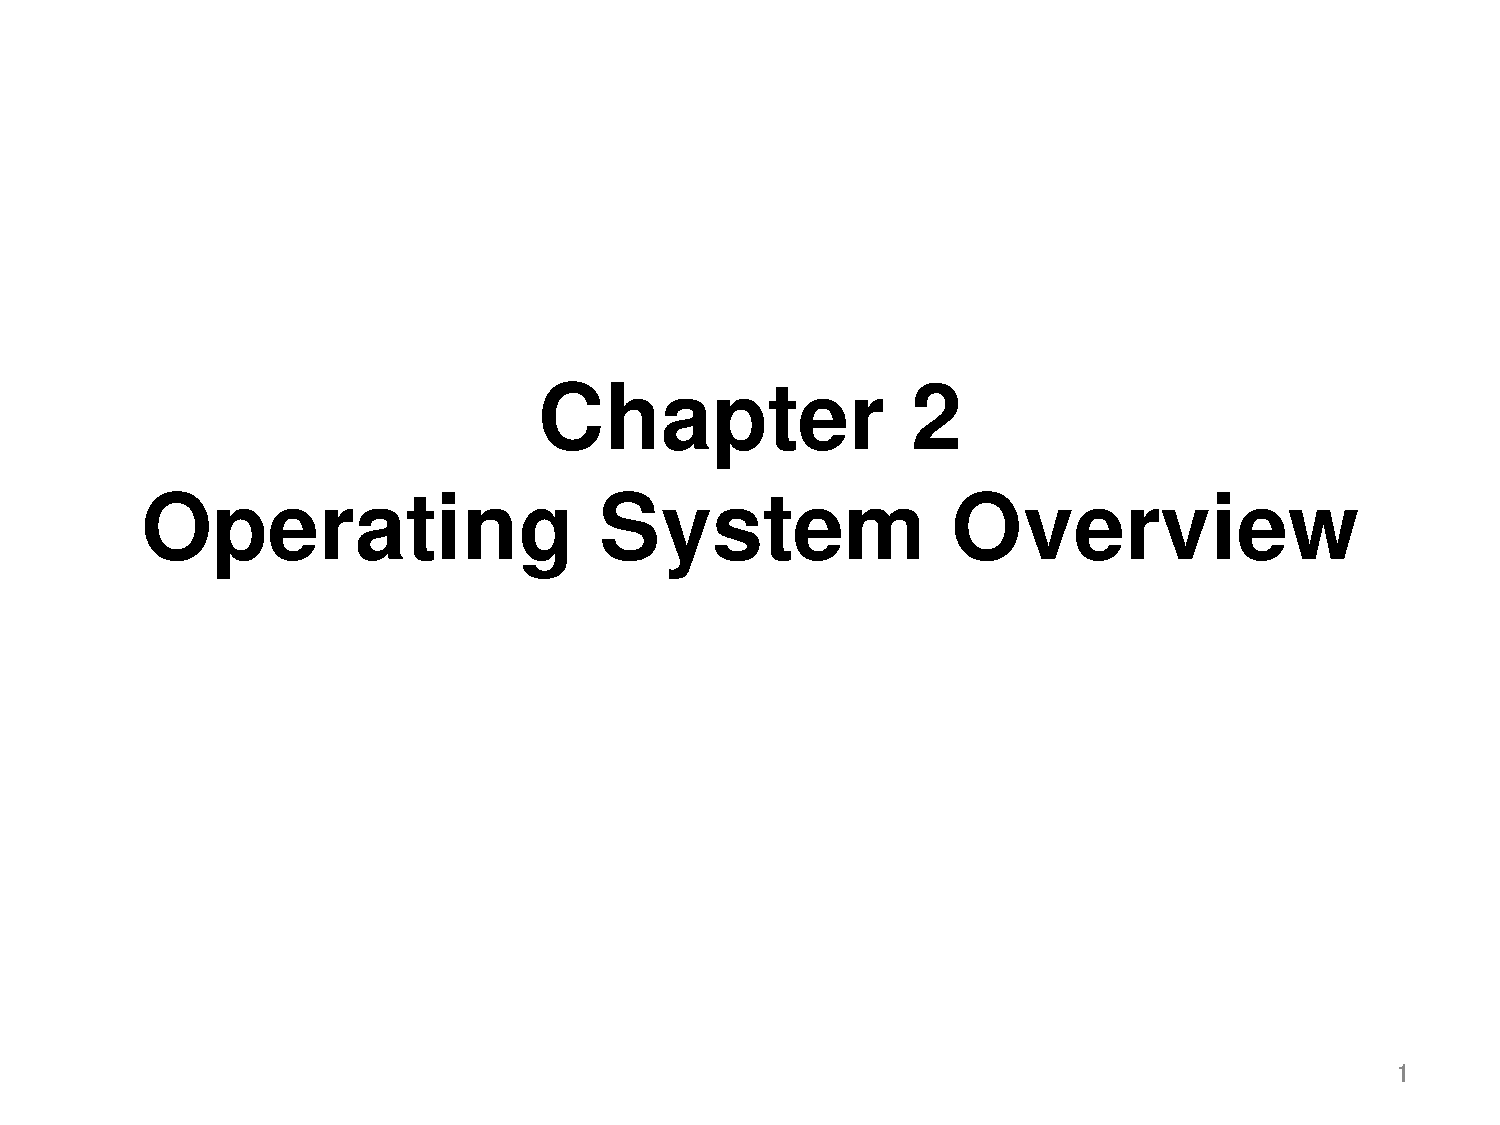
\includepdf[page=2]{03.pdf}
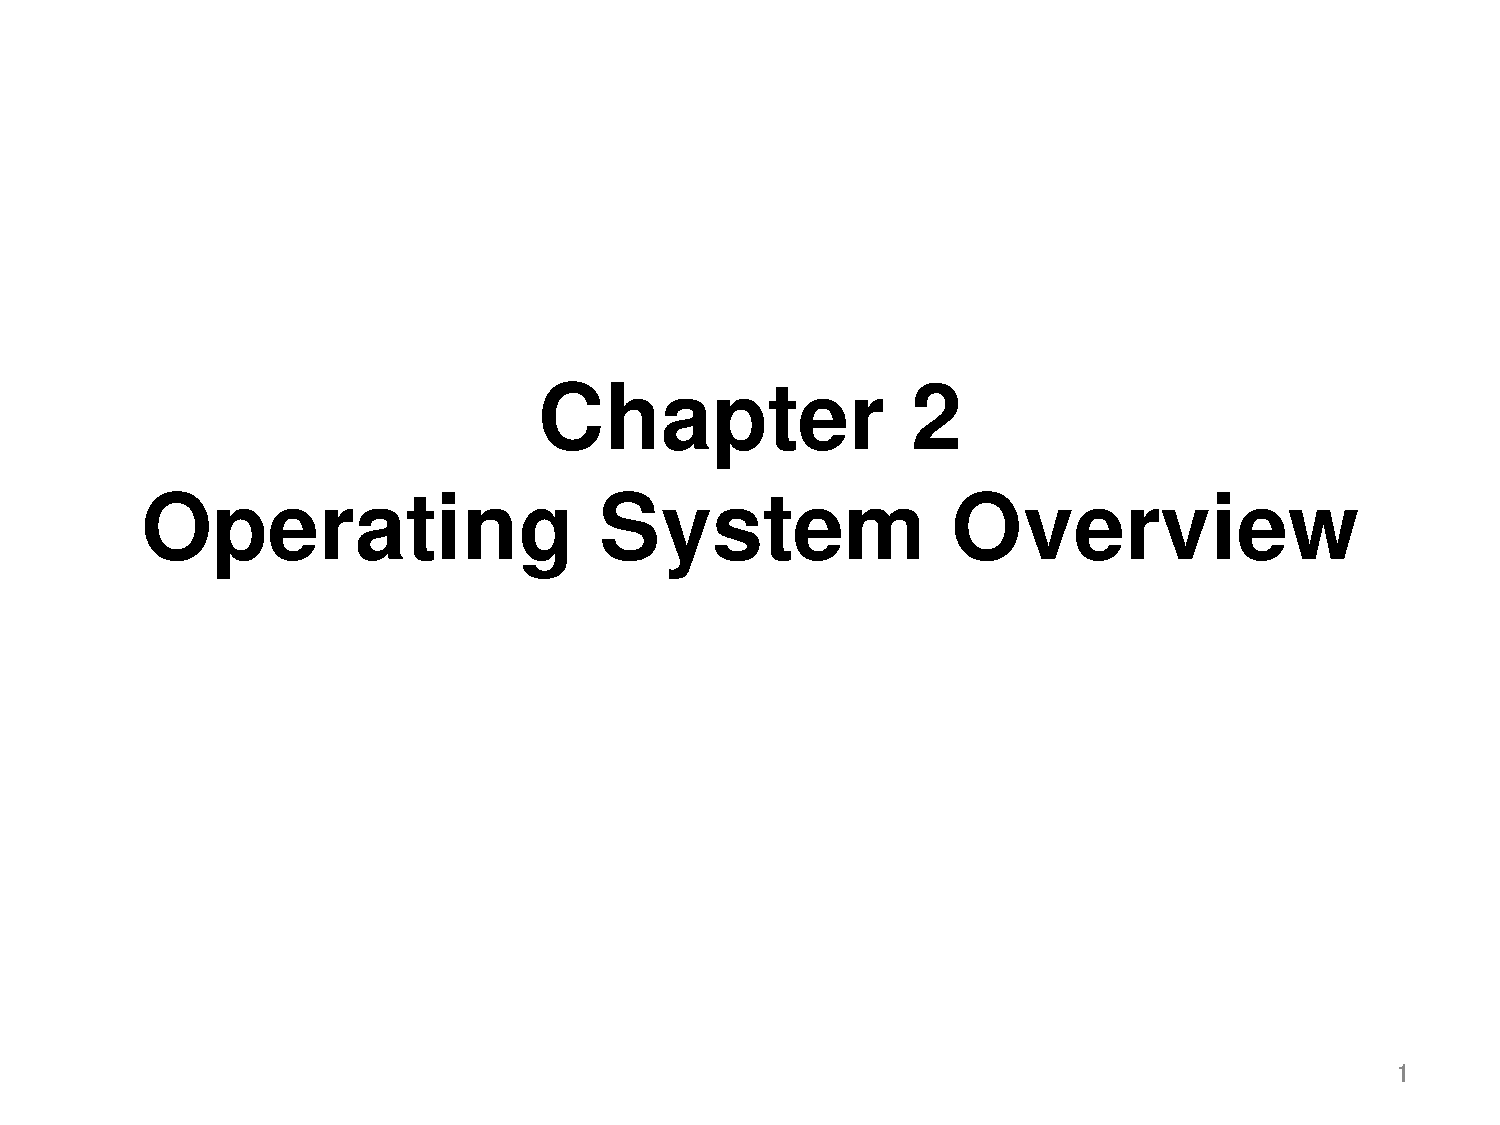
\includepdf[page=3]{03.pdf}
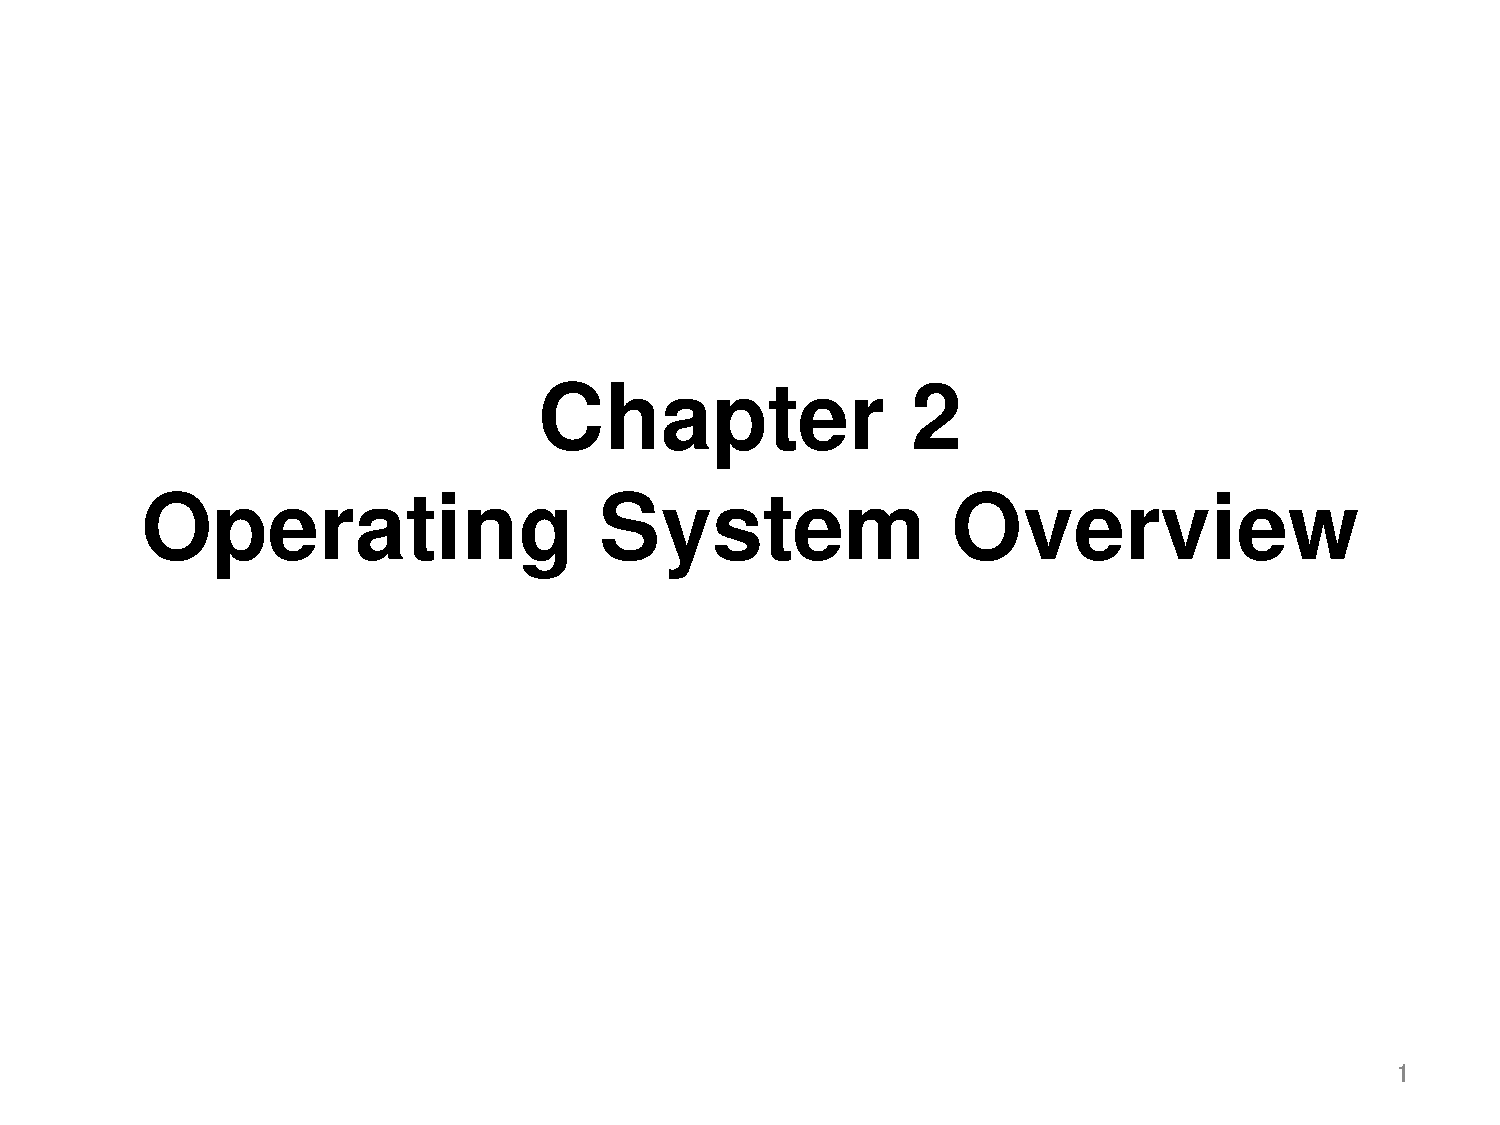
\includepdf[page=4]{03.pdf}
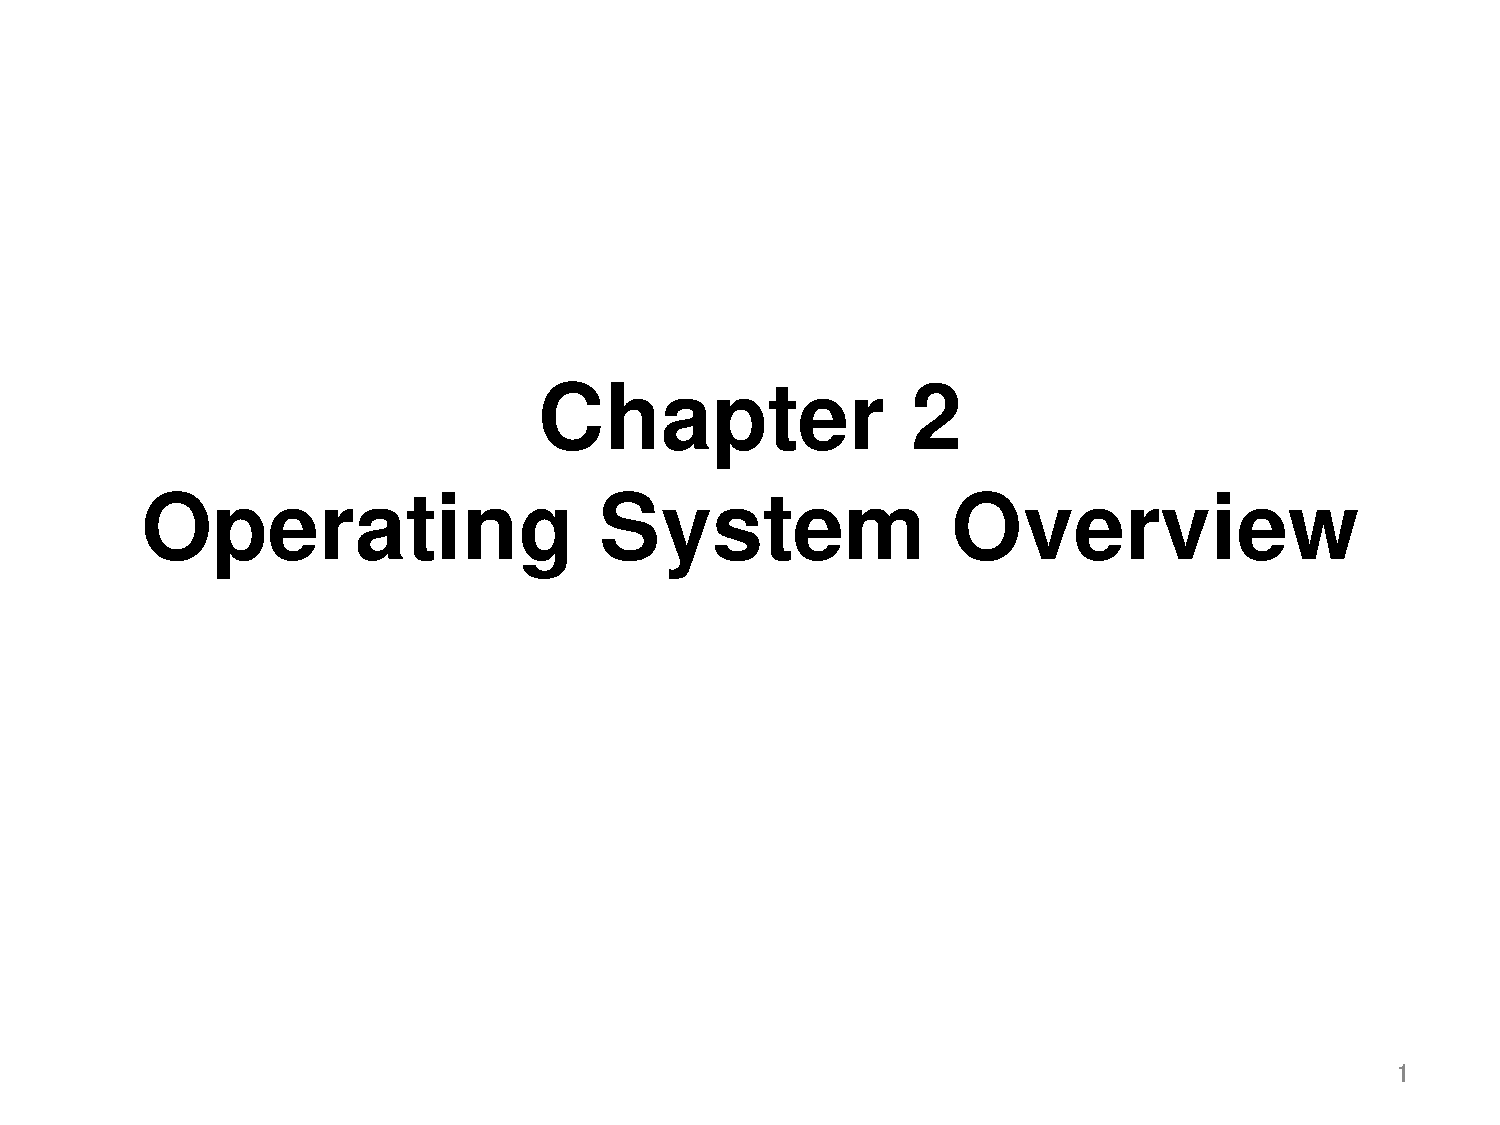
\includepdf[page=5]{03.pdf}
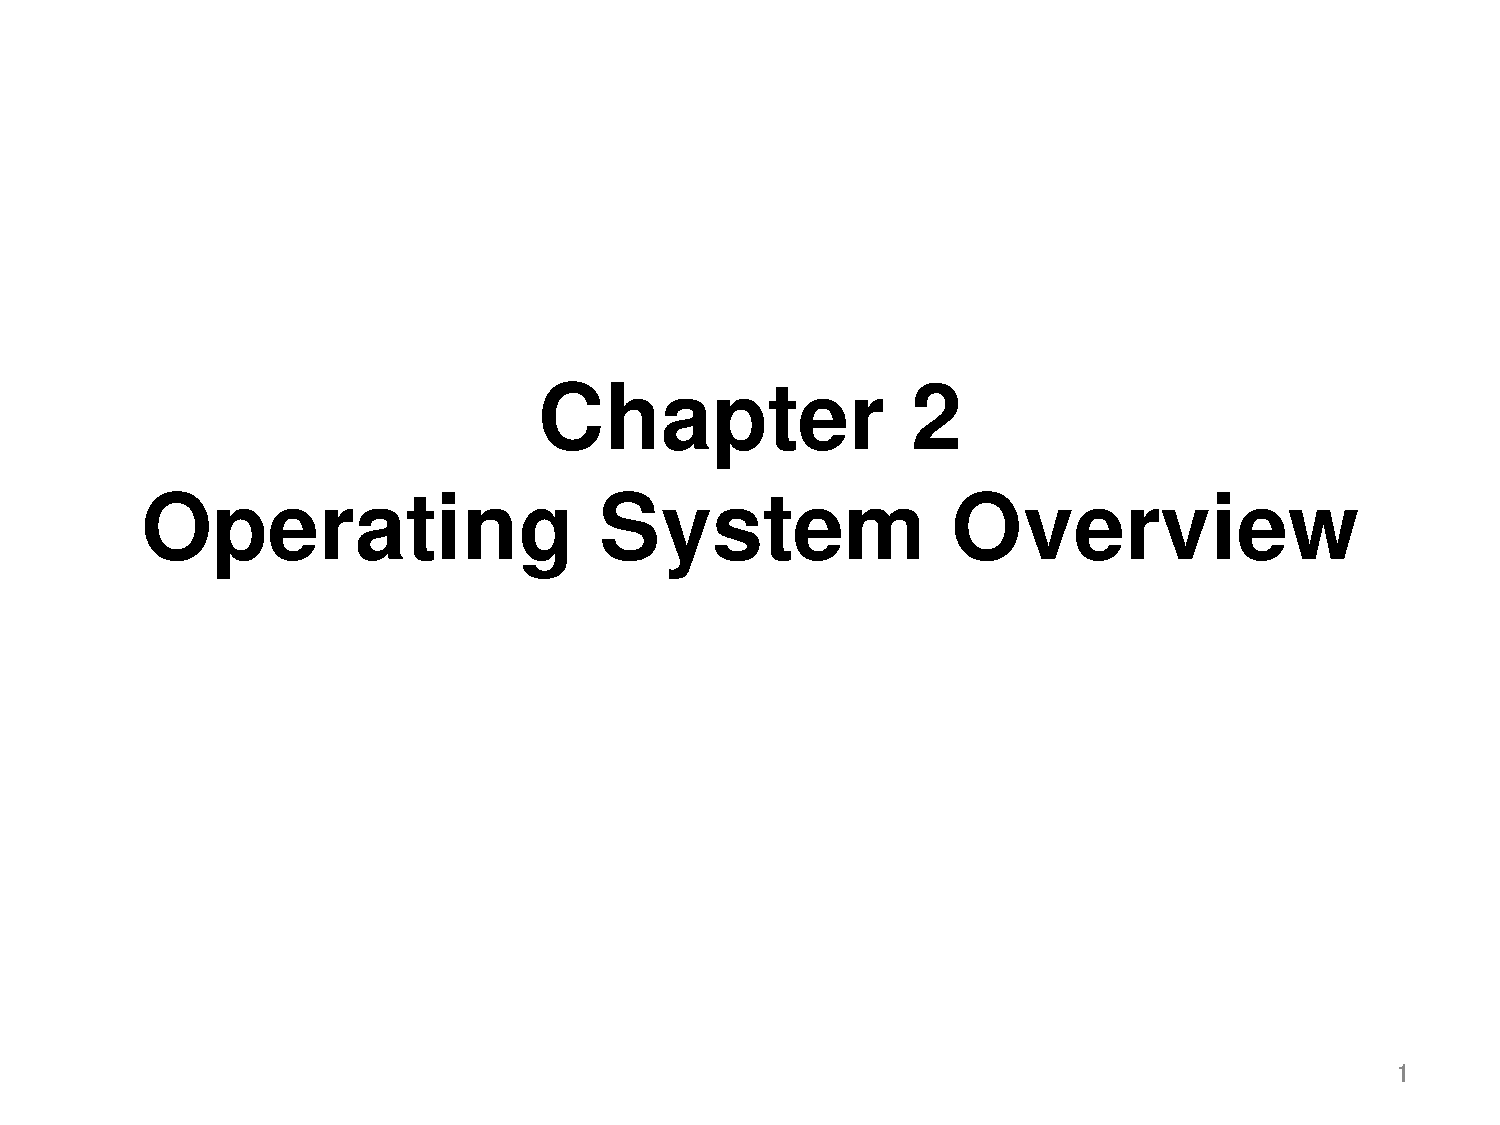
\includepdf[page=6]{03.pdf}
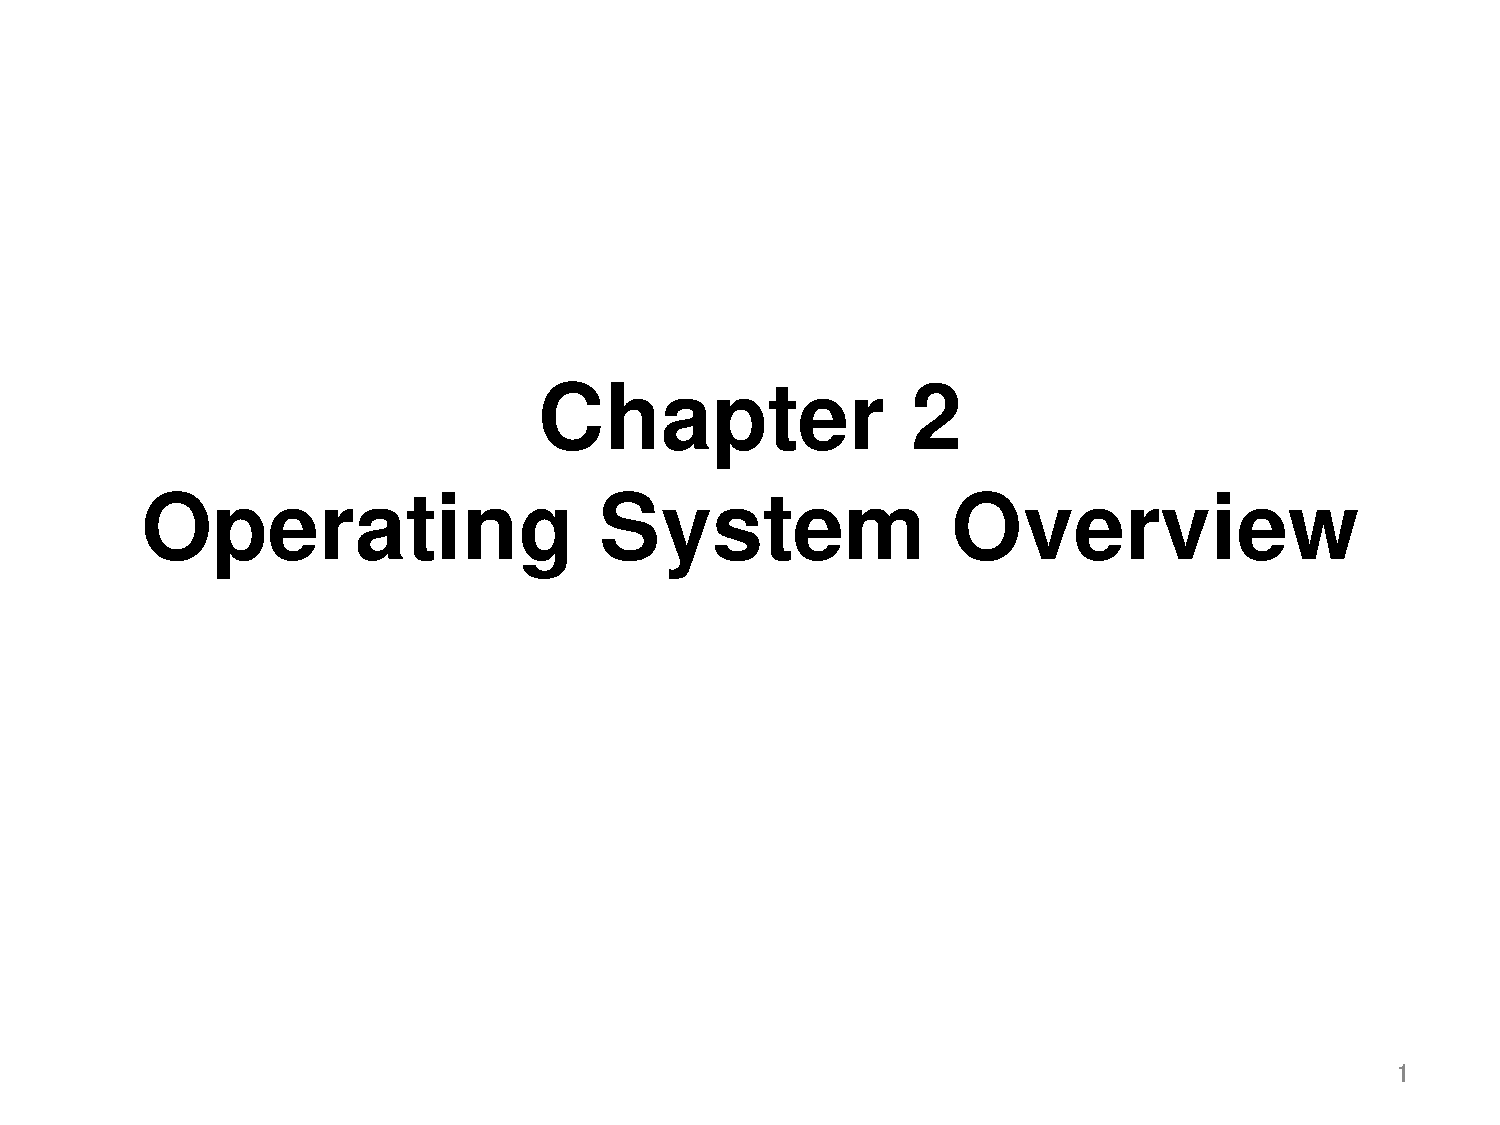
\includepdf[page=7]{03.pdf}
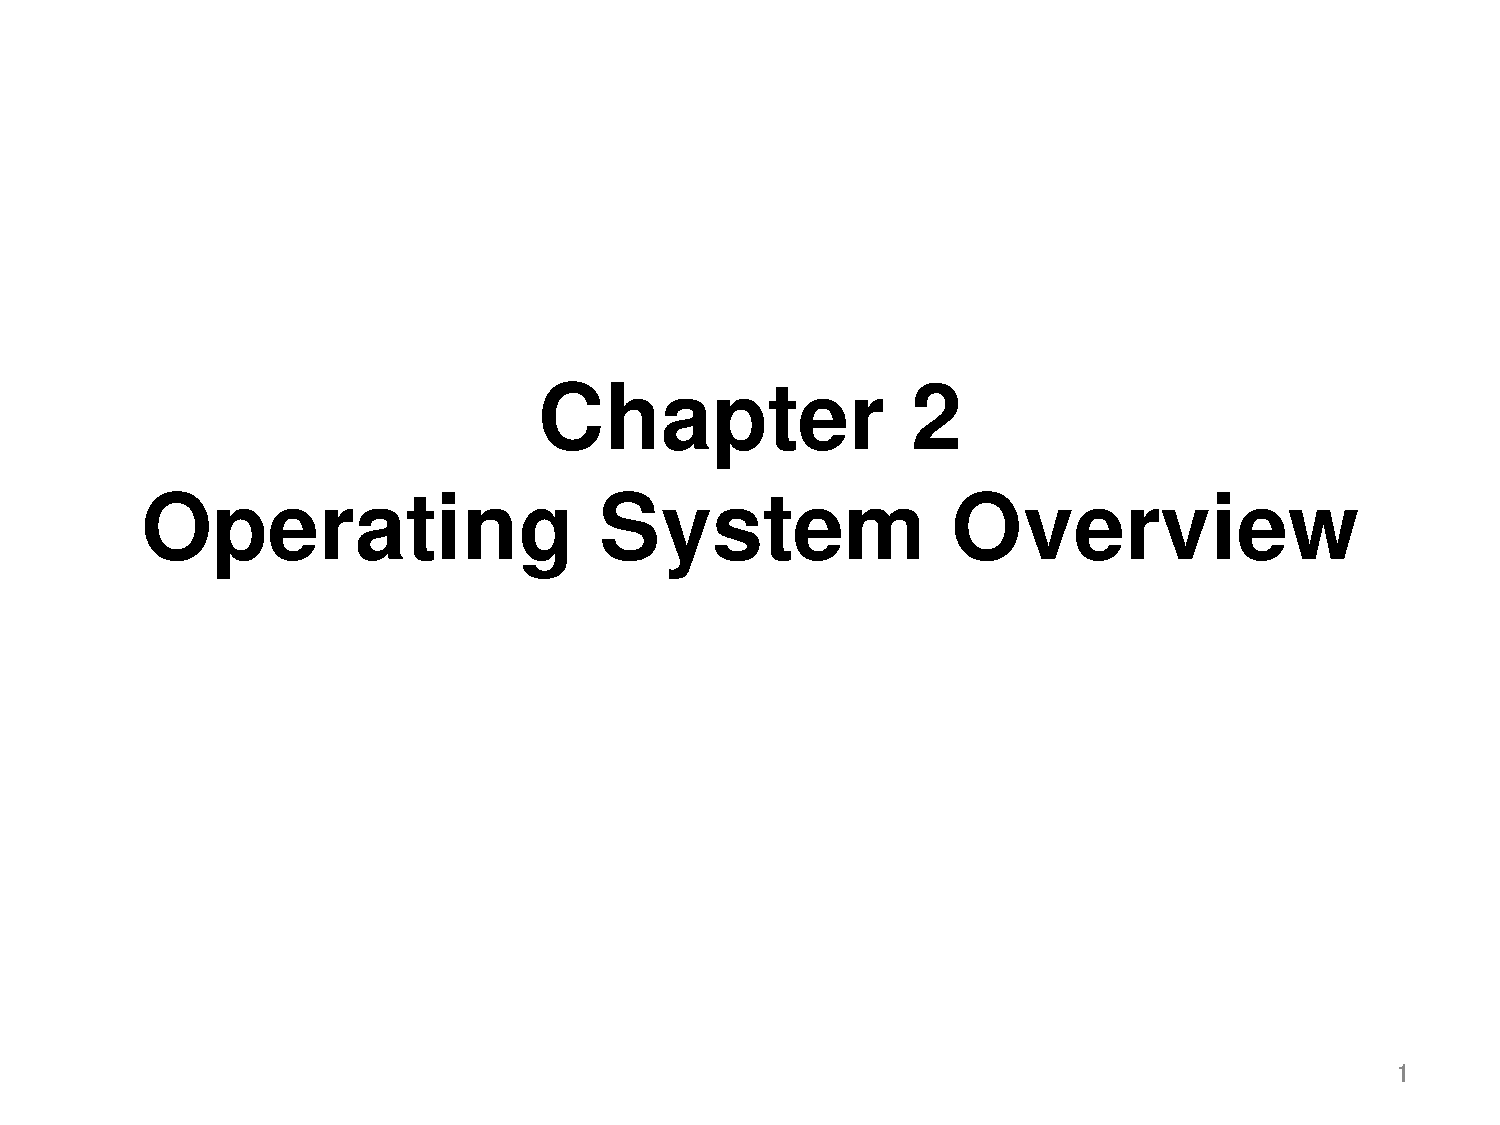
\includepdf[page=8]{03.pdf}
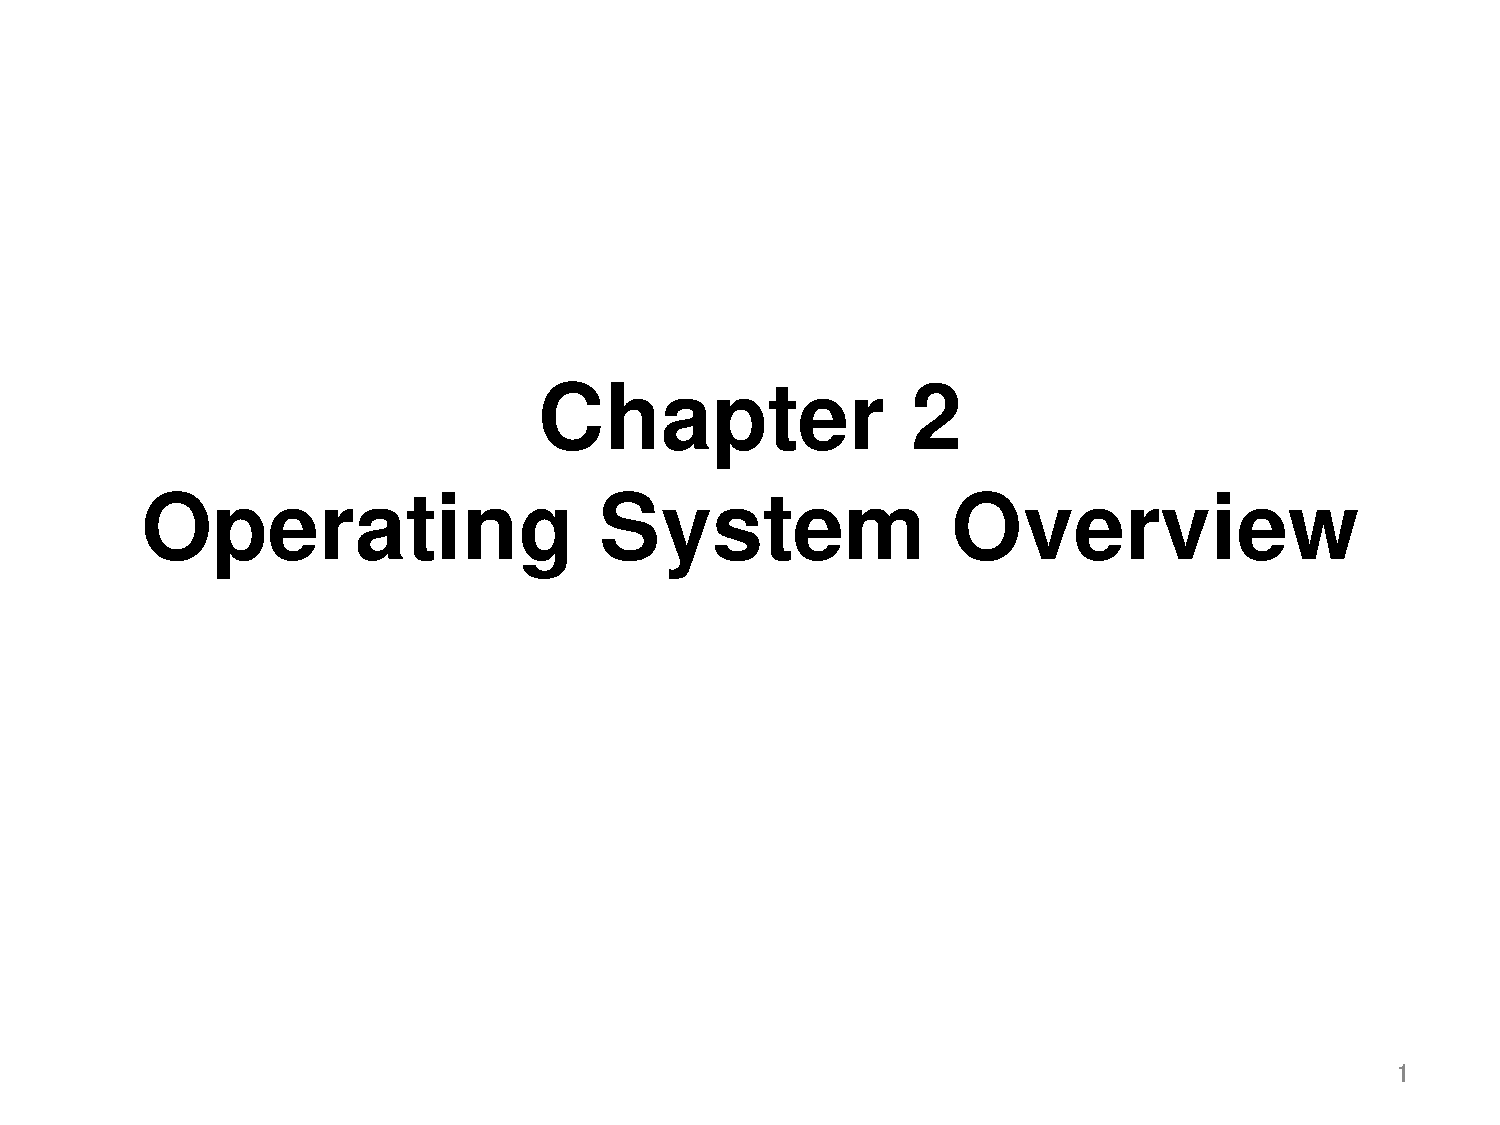
\includepdf[page=9]{03.pdf}
The operating system is a program that gets executed which means that the user program must relinquish control of the processor (this is done through interrupts)
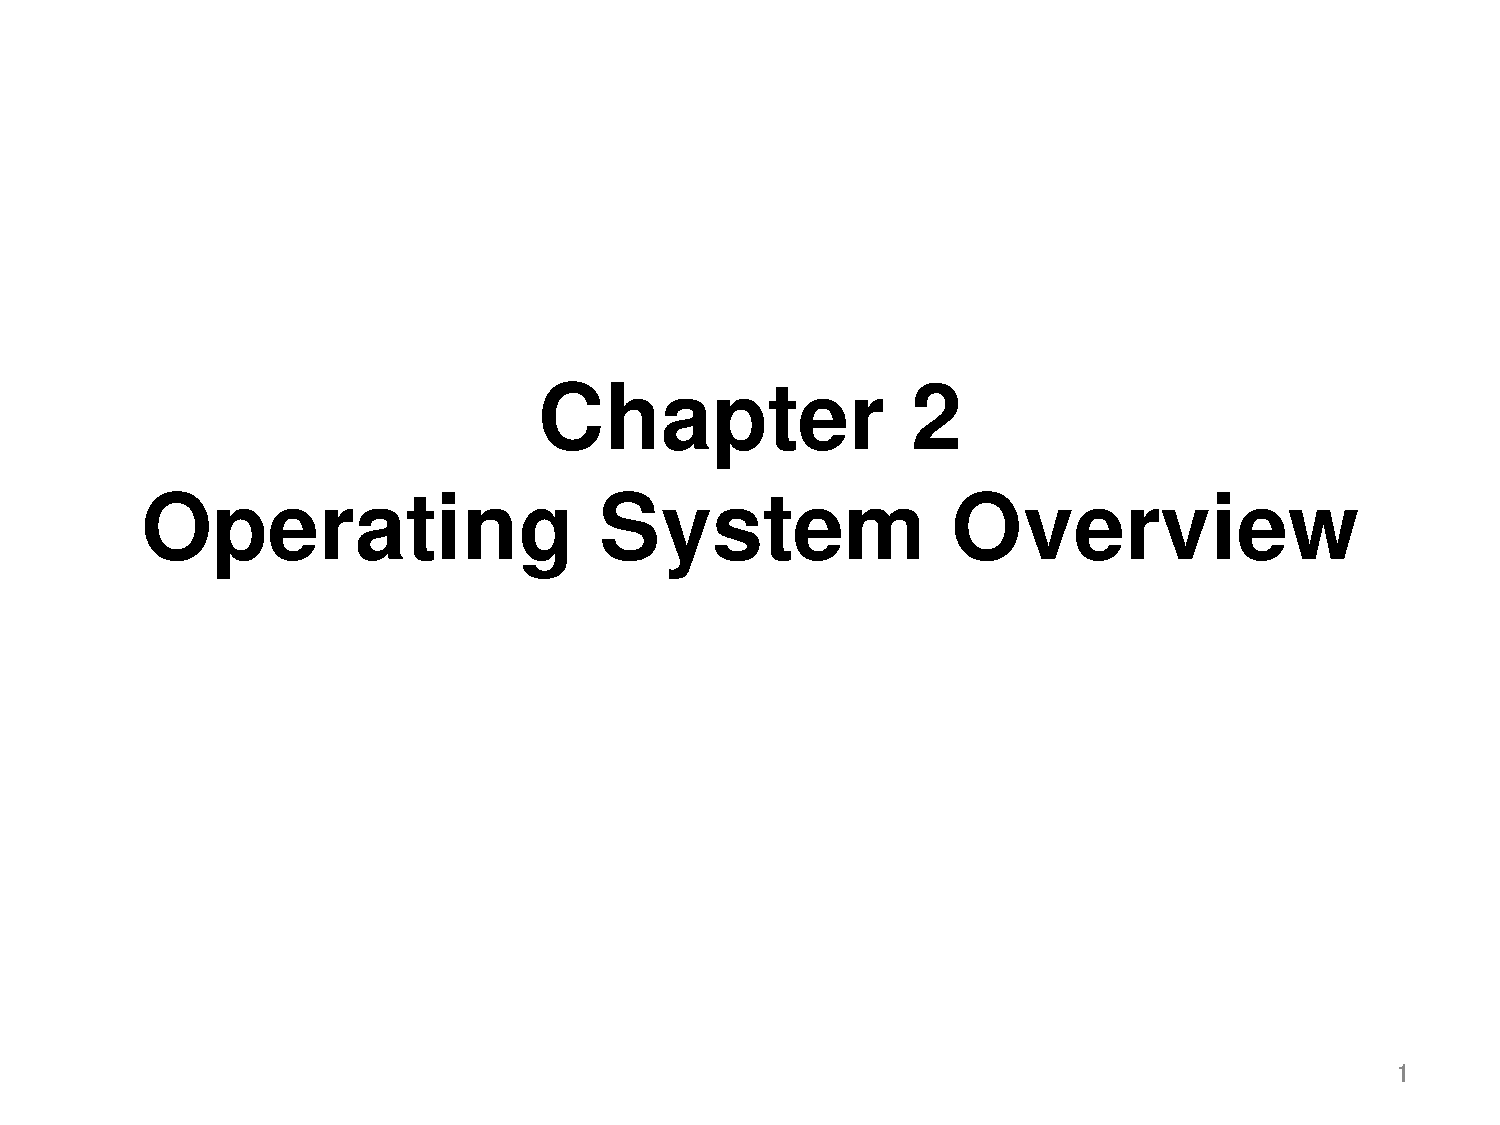
\includepdf[page=10]{03.pdf}
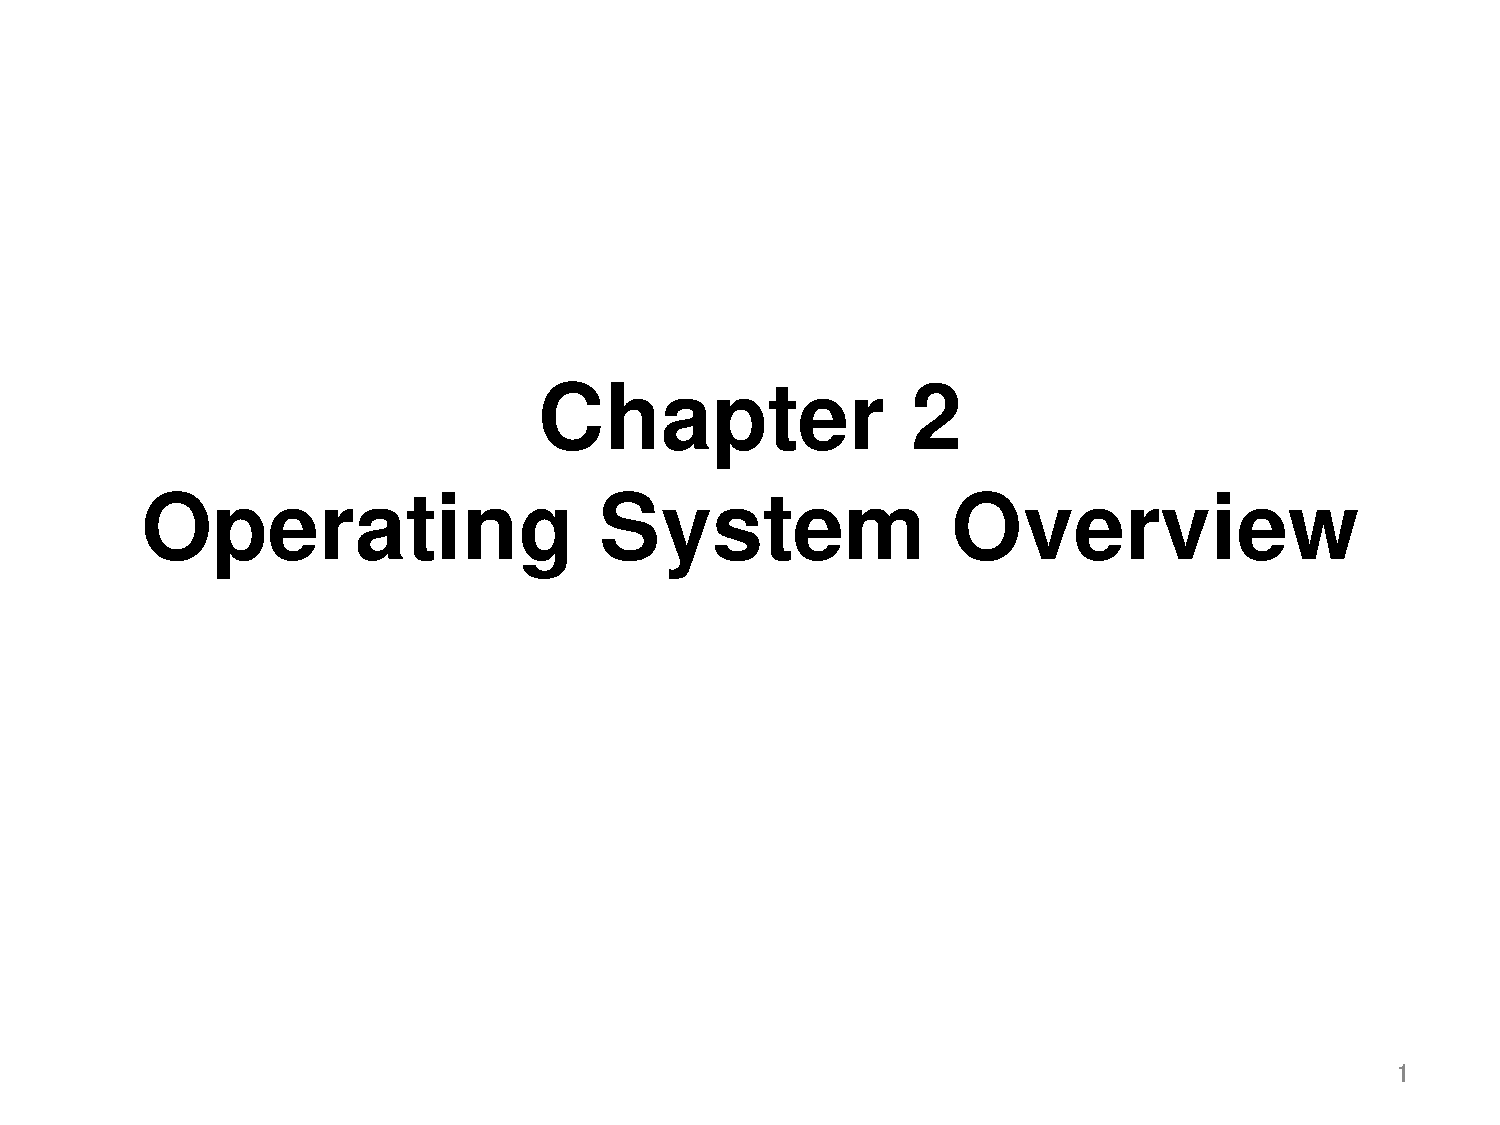
\includepdf[page=11]{03.pdf}
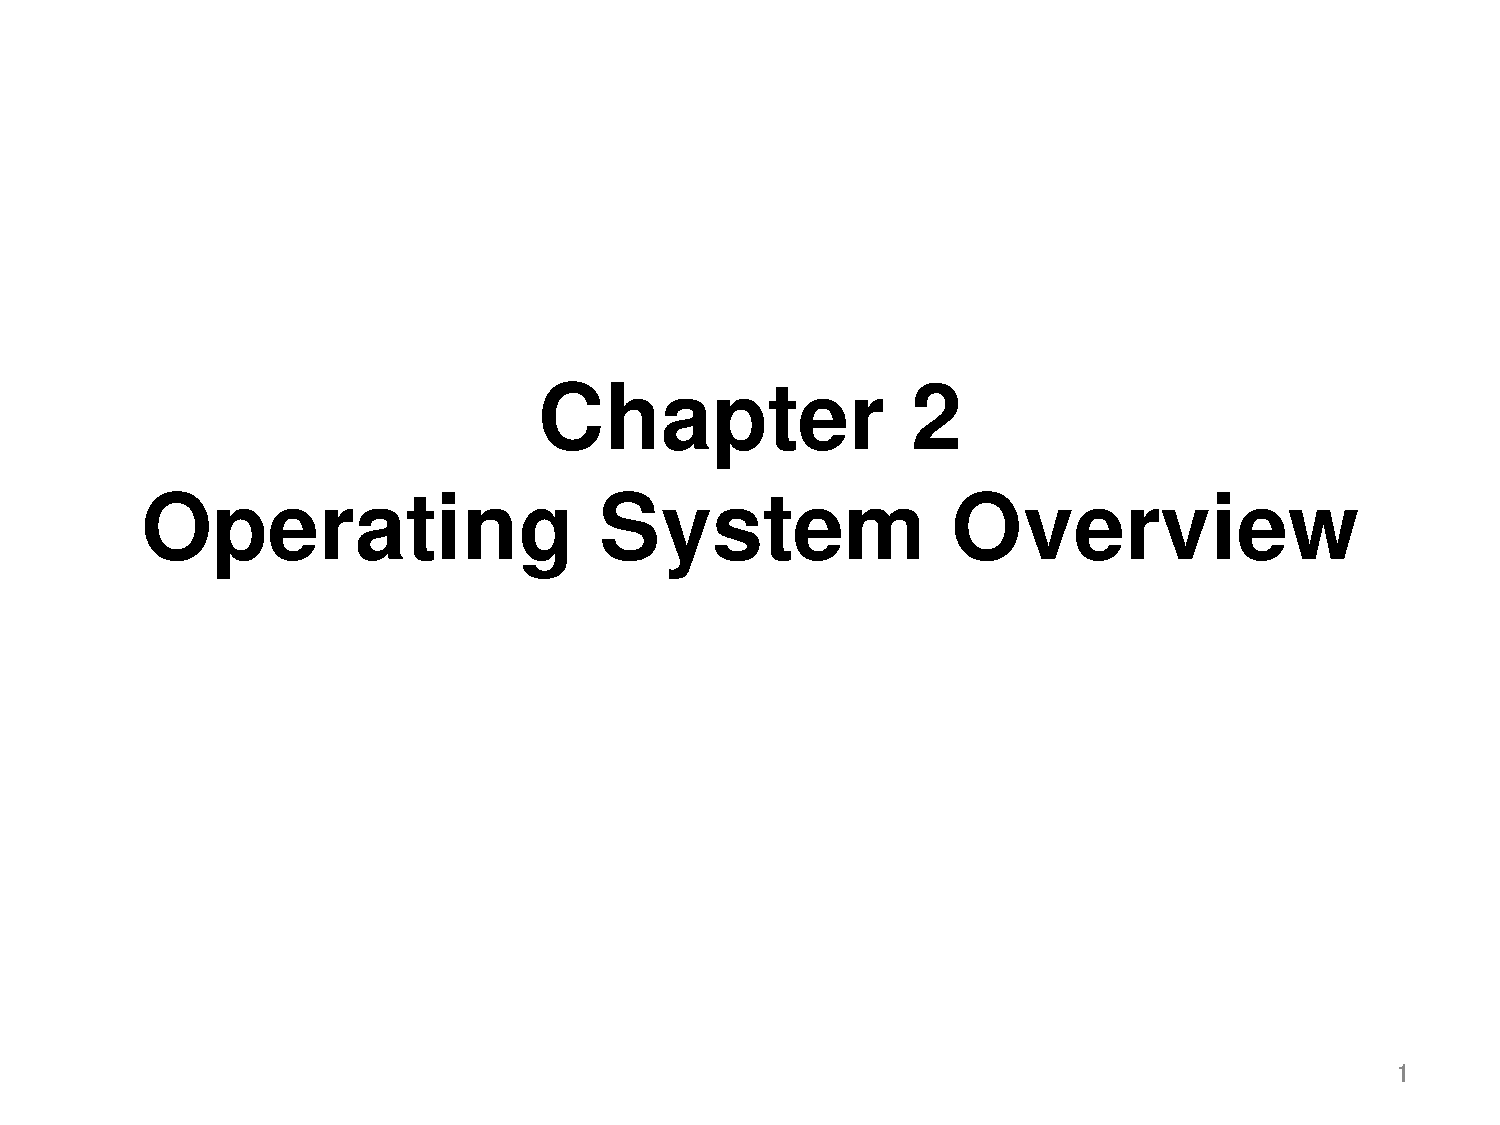
\includepdf[page=12]{03.pdf}
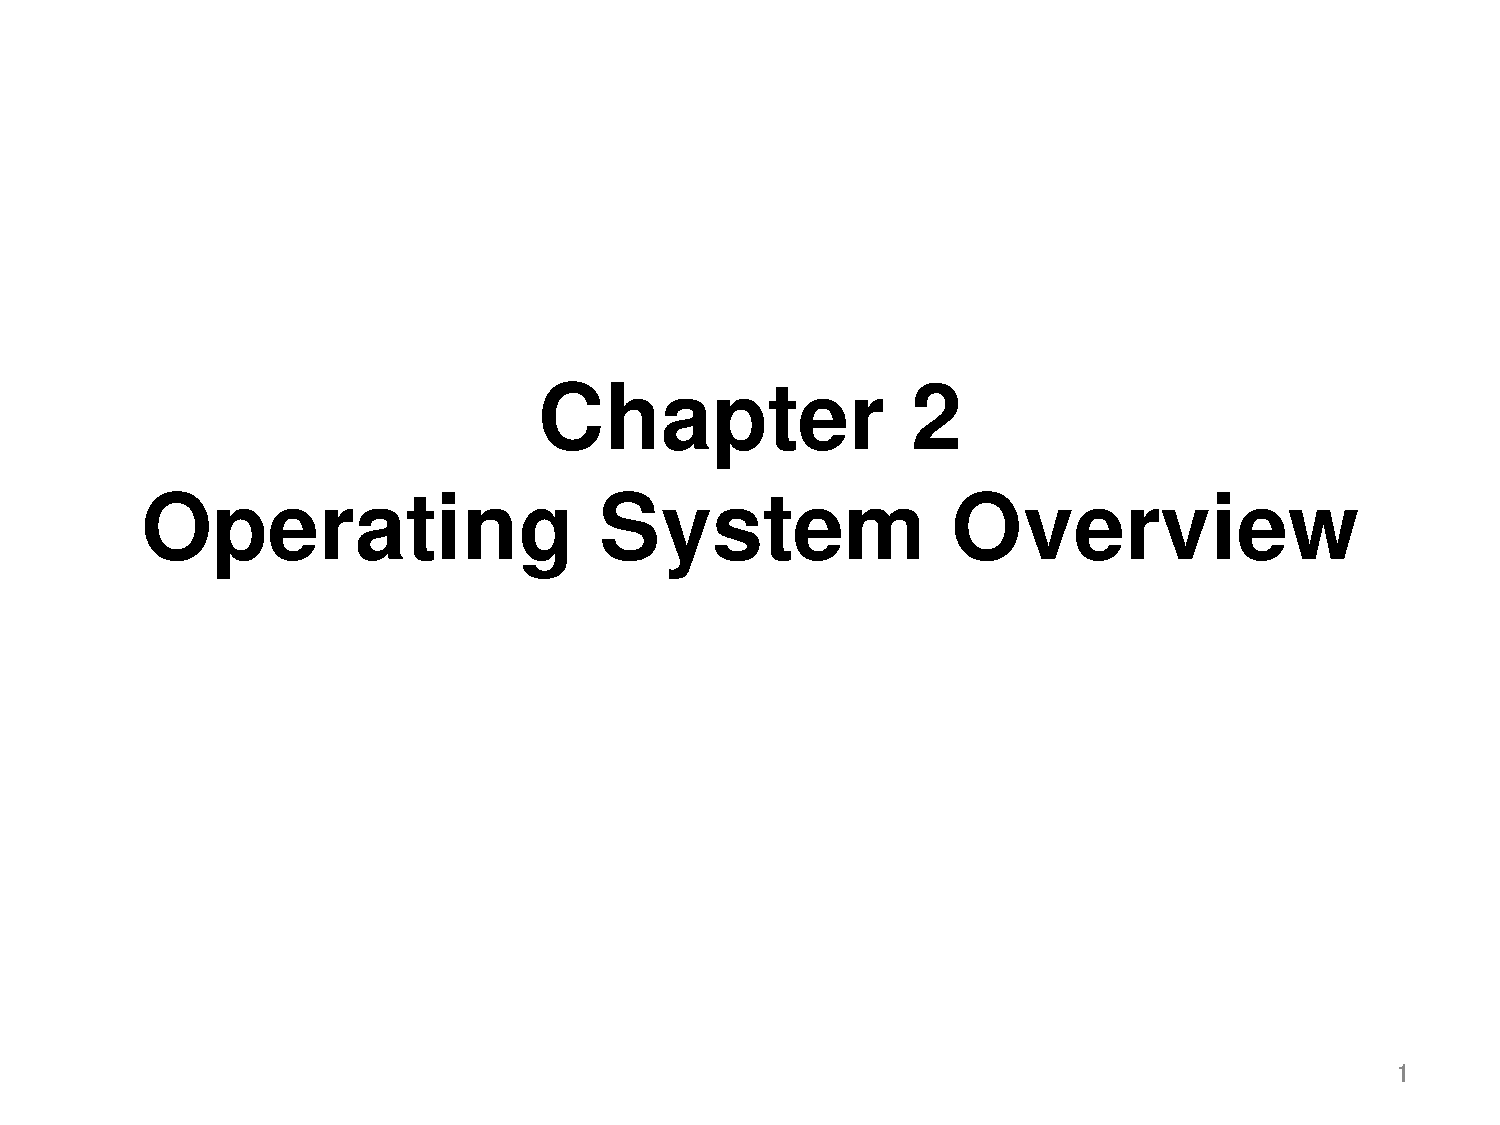
\includepdf[page=13]{03.pdf}
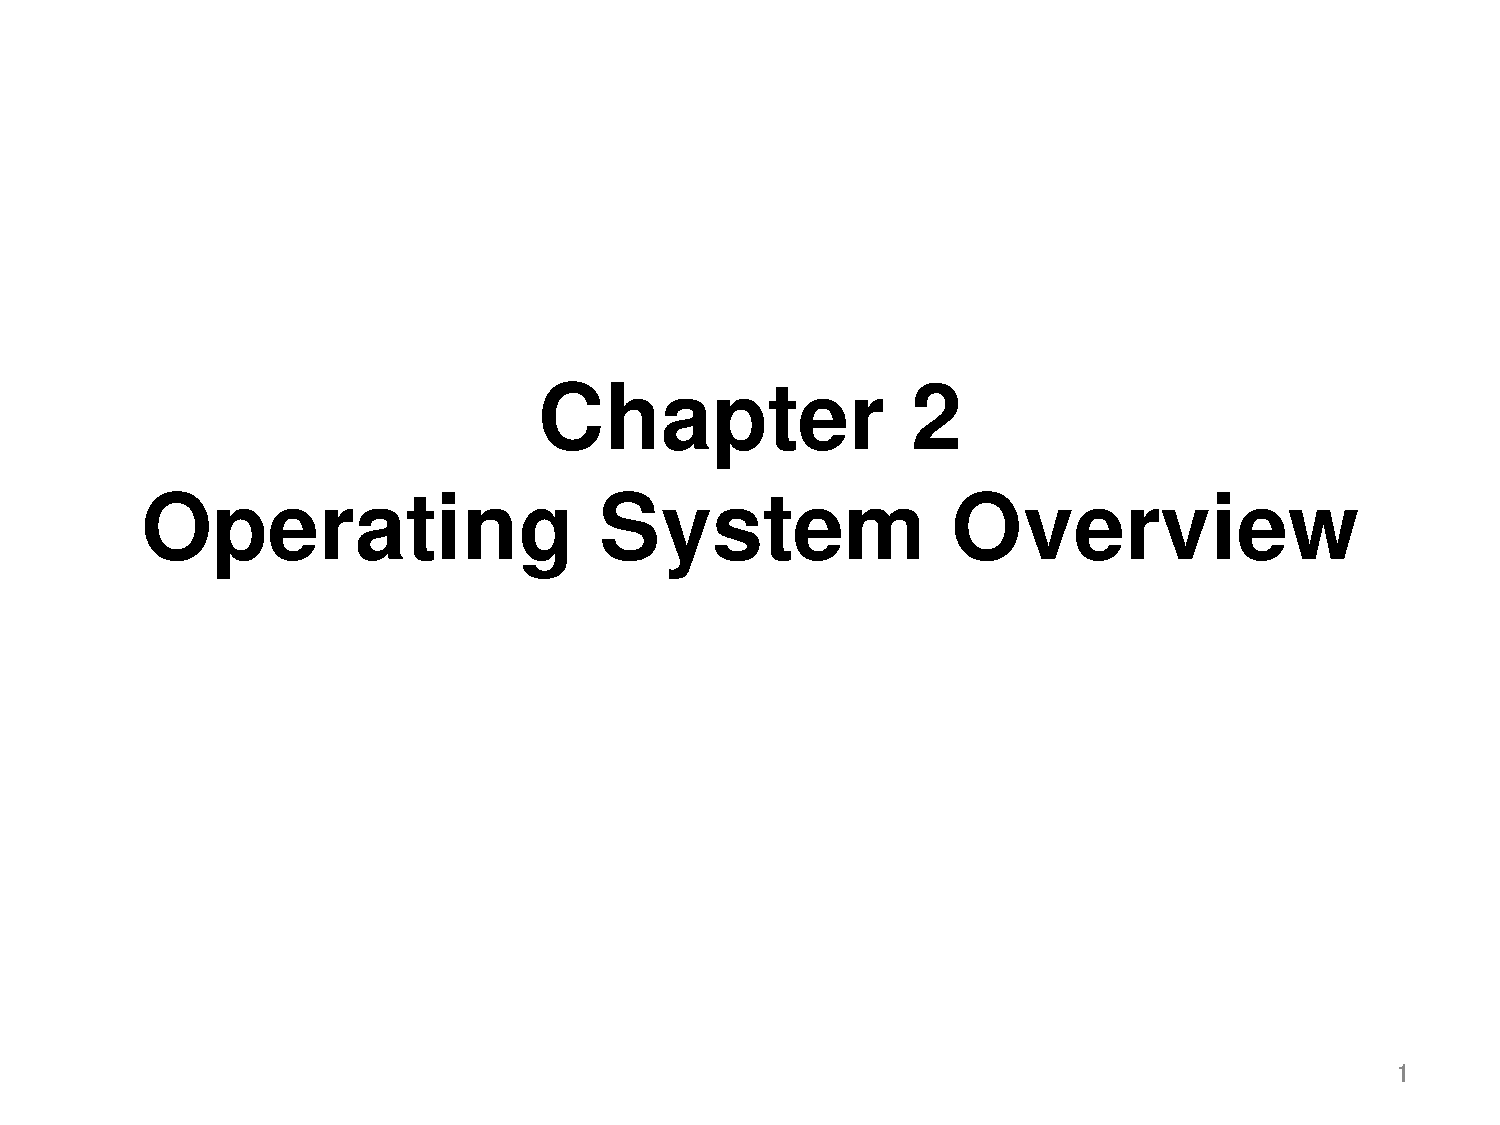
\includepdf[page=14]{03.pdf}
Developement on these machines was very hard because you needed physical access to one of a few machines resulting in large amounts of downtime between tests. There was a lot of setup required to run the program (load all of the things)
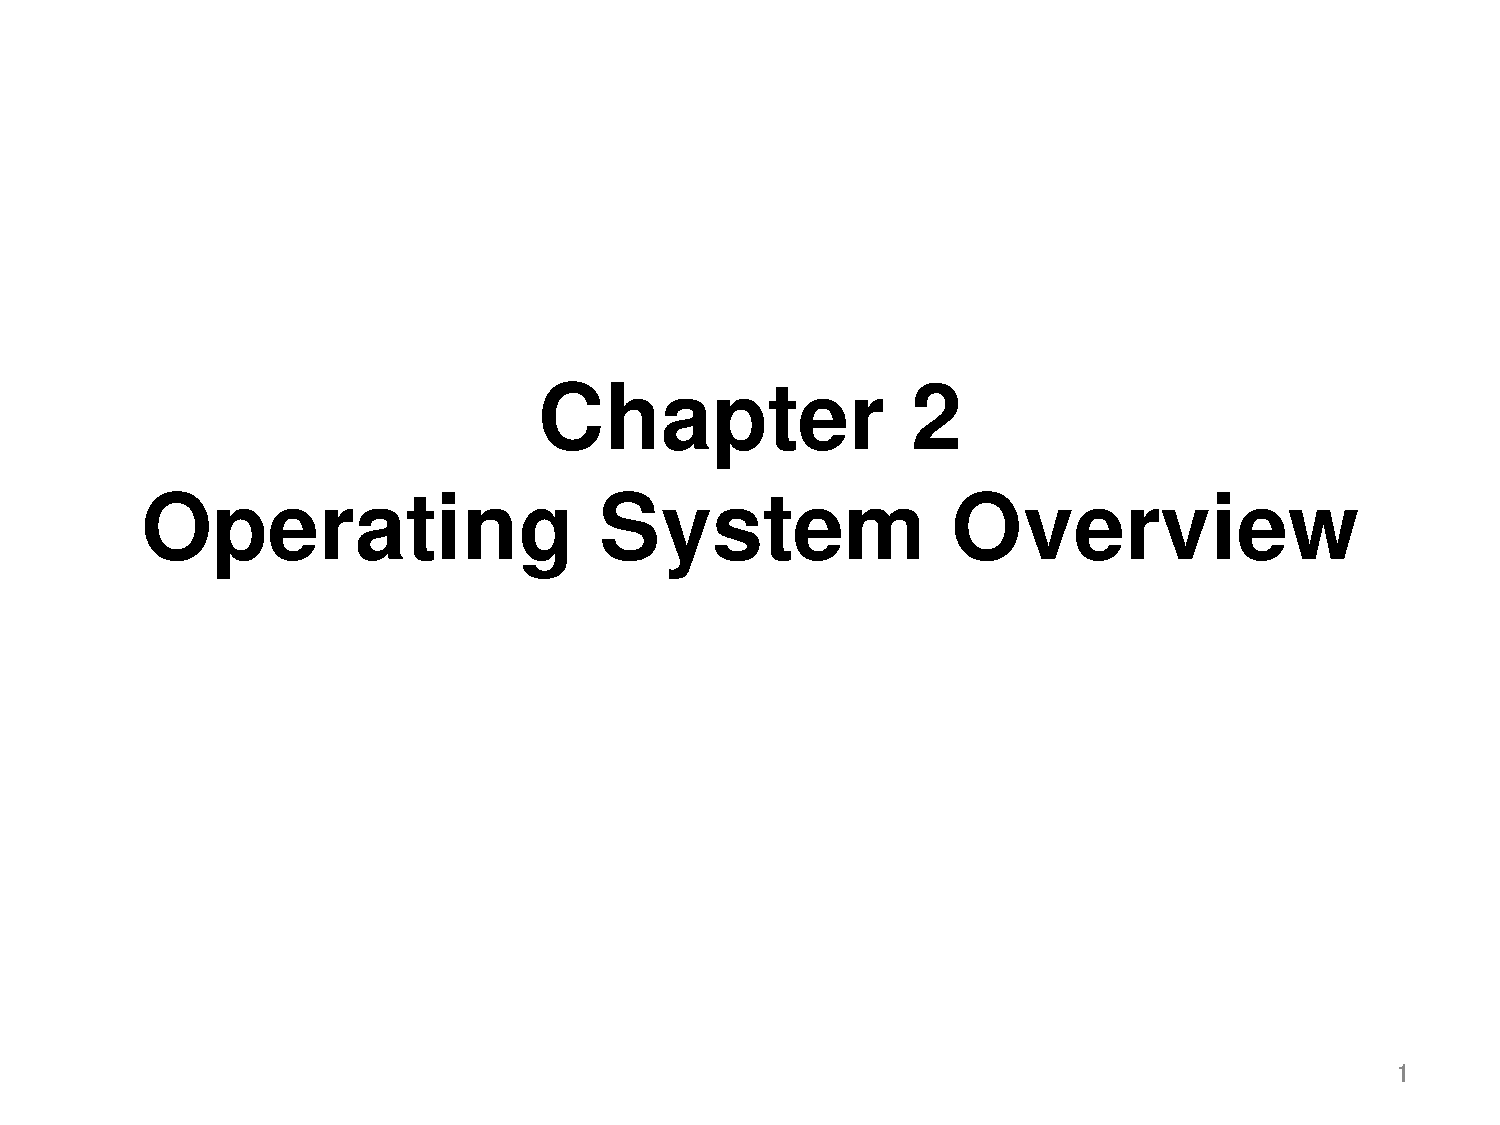
\includepdf[page=15]{03.pdf}
This lets us bunch operations together to make things run much faster. The problem with this was security, you could override the monitor to make it so that your code had a higher priority.
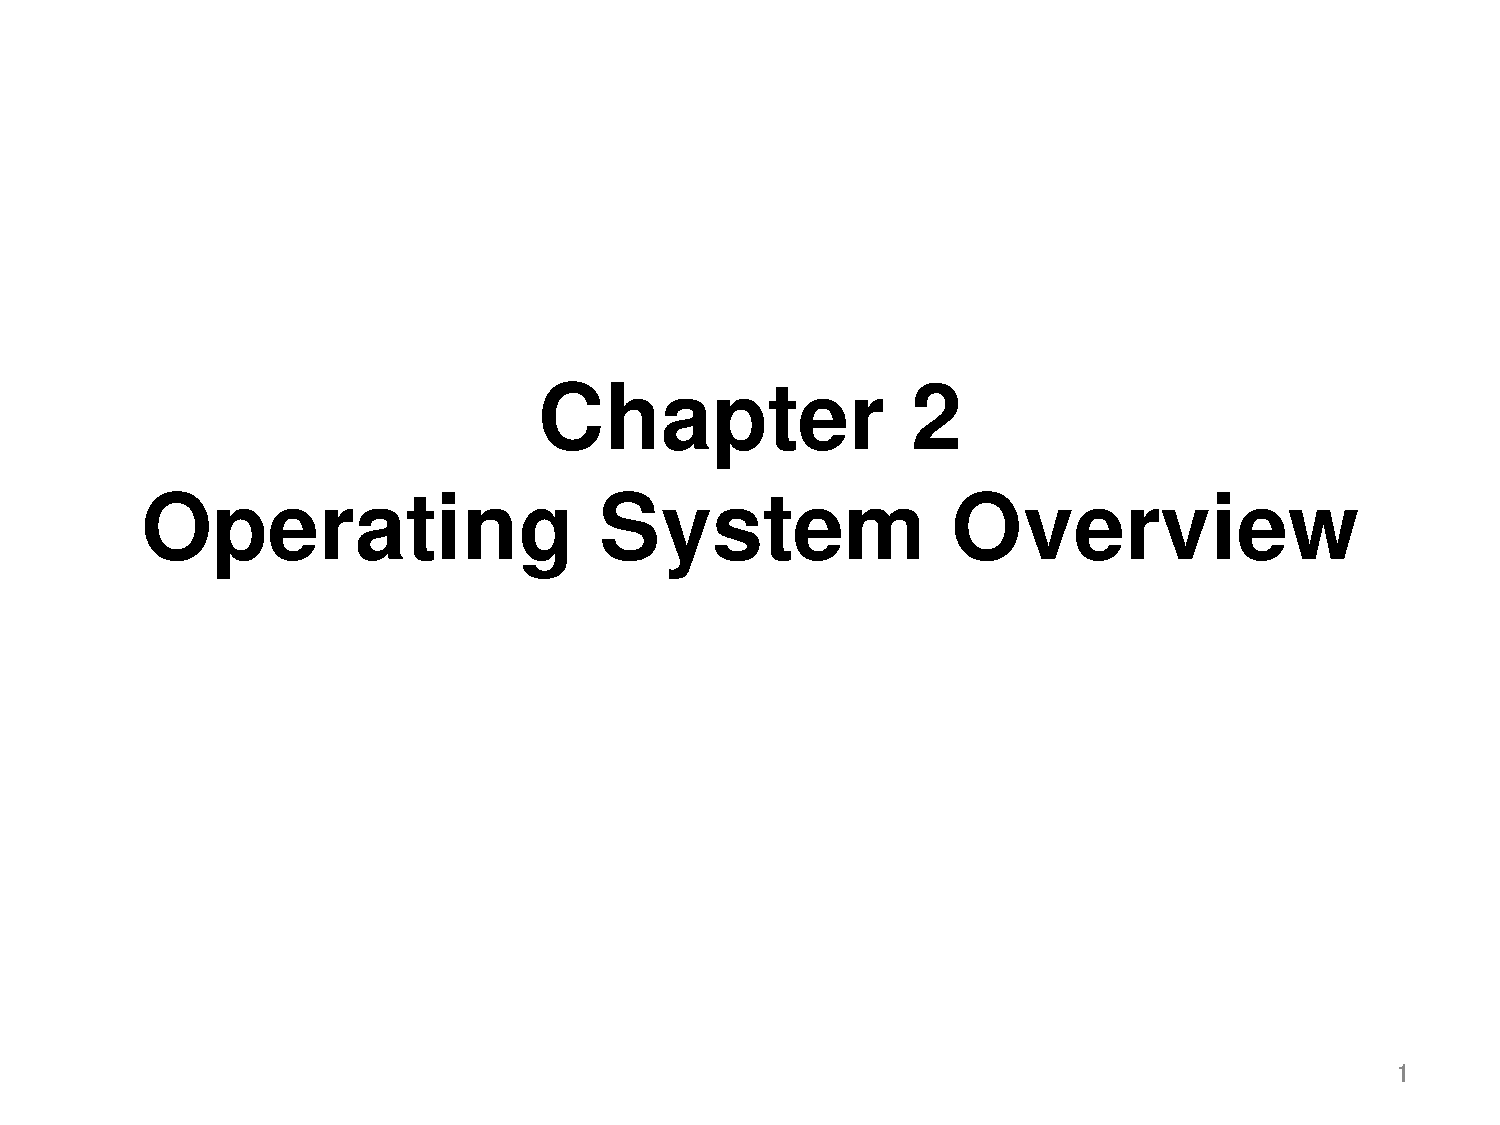
\includepdf[page=16]{03.pdf}
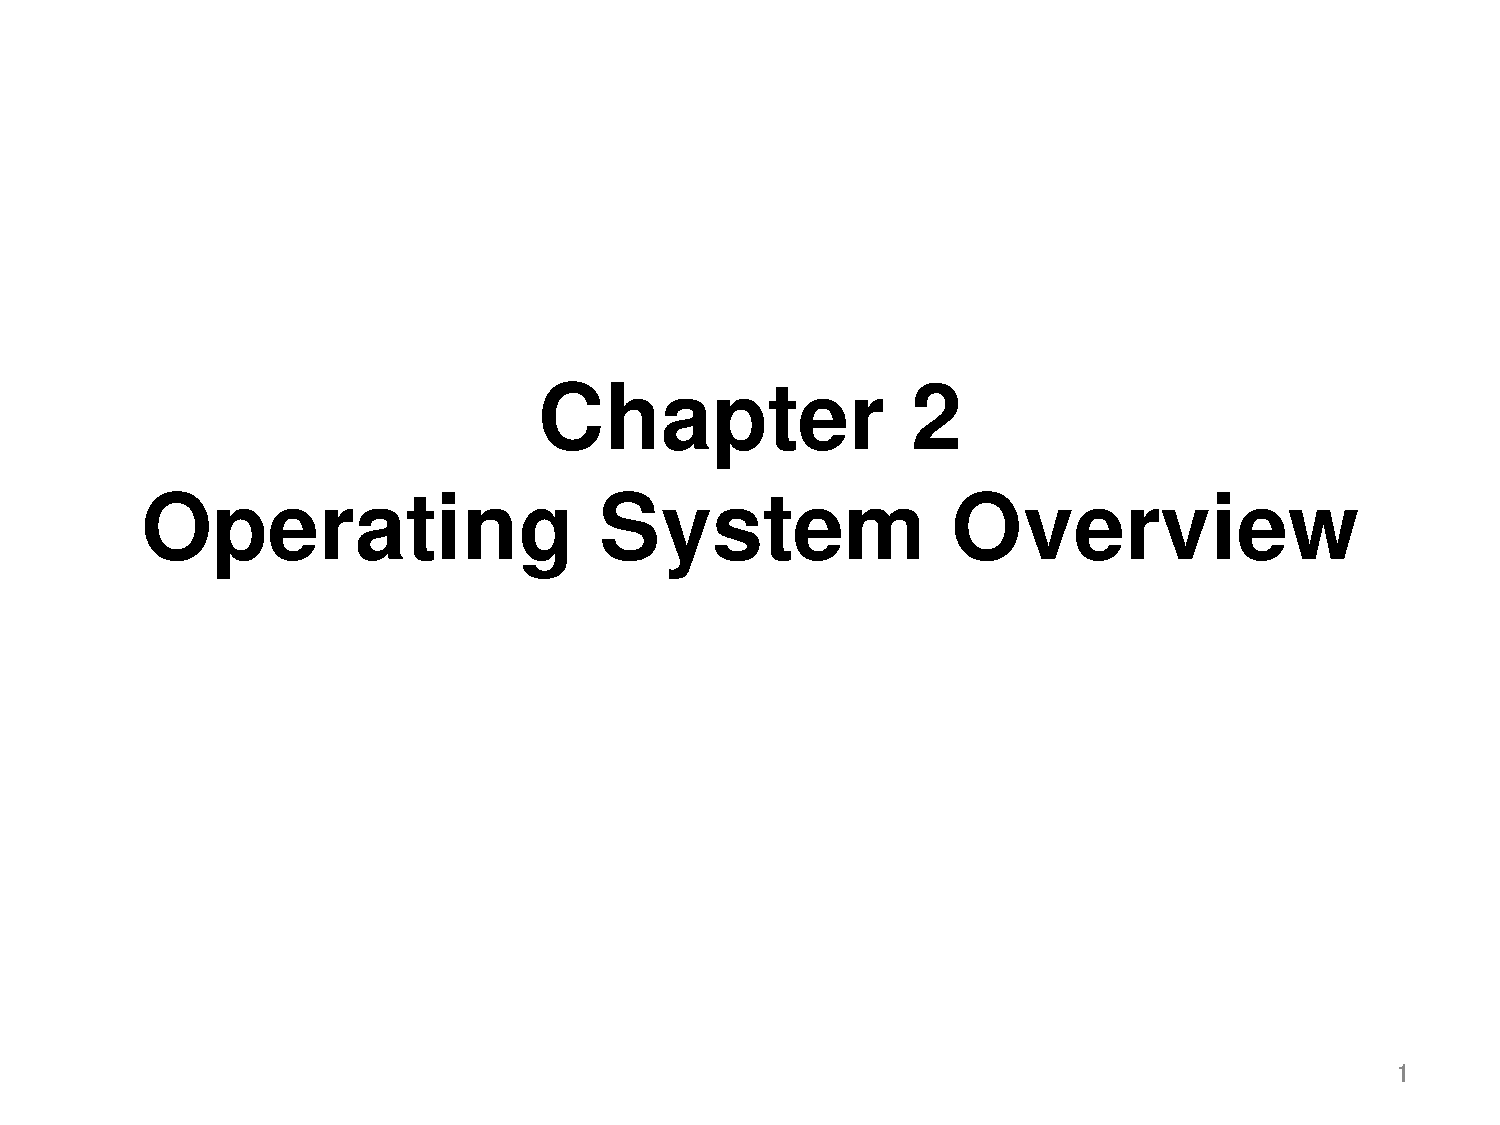
\includepdf[page=17]{03.pdf}
This helped stop people from overriding the monitor making things much more secure. Similarly is makes things more efficient by preventing one job from monopolizing the system. The monitor was a periodic interrupt that checked on things and jumped between programs as needed.
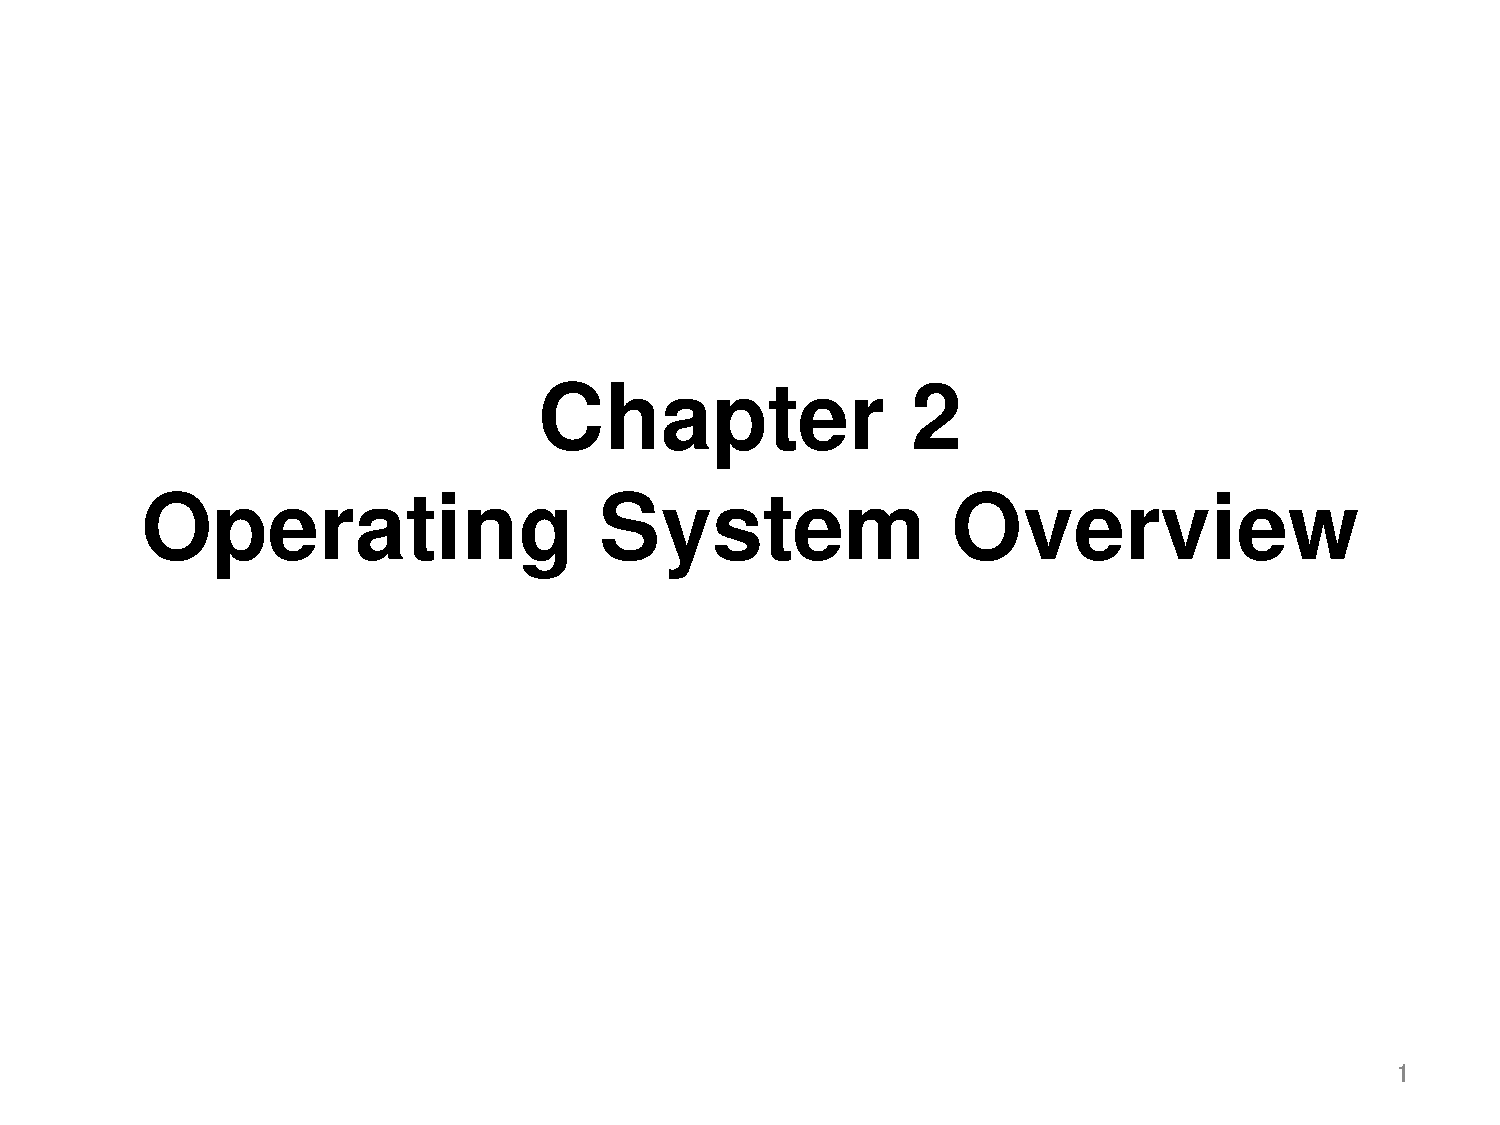
\includepdf[page=18]{03.pdf}
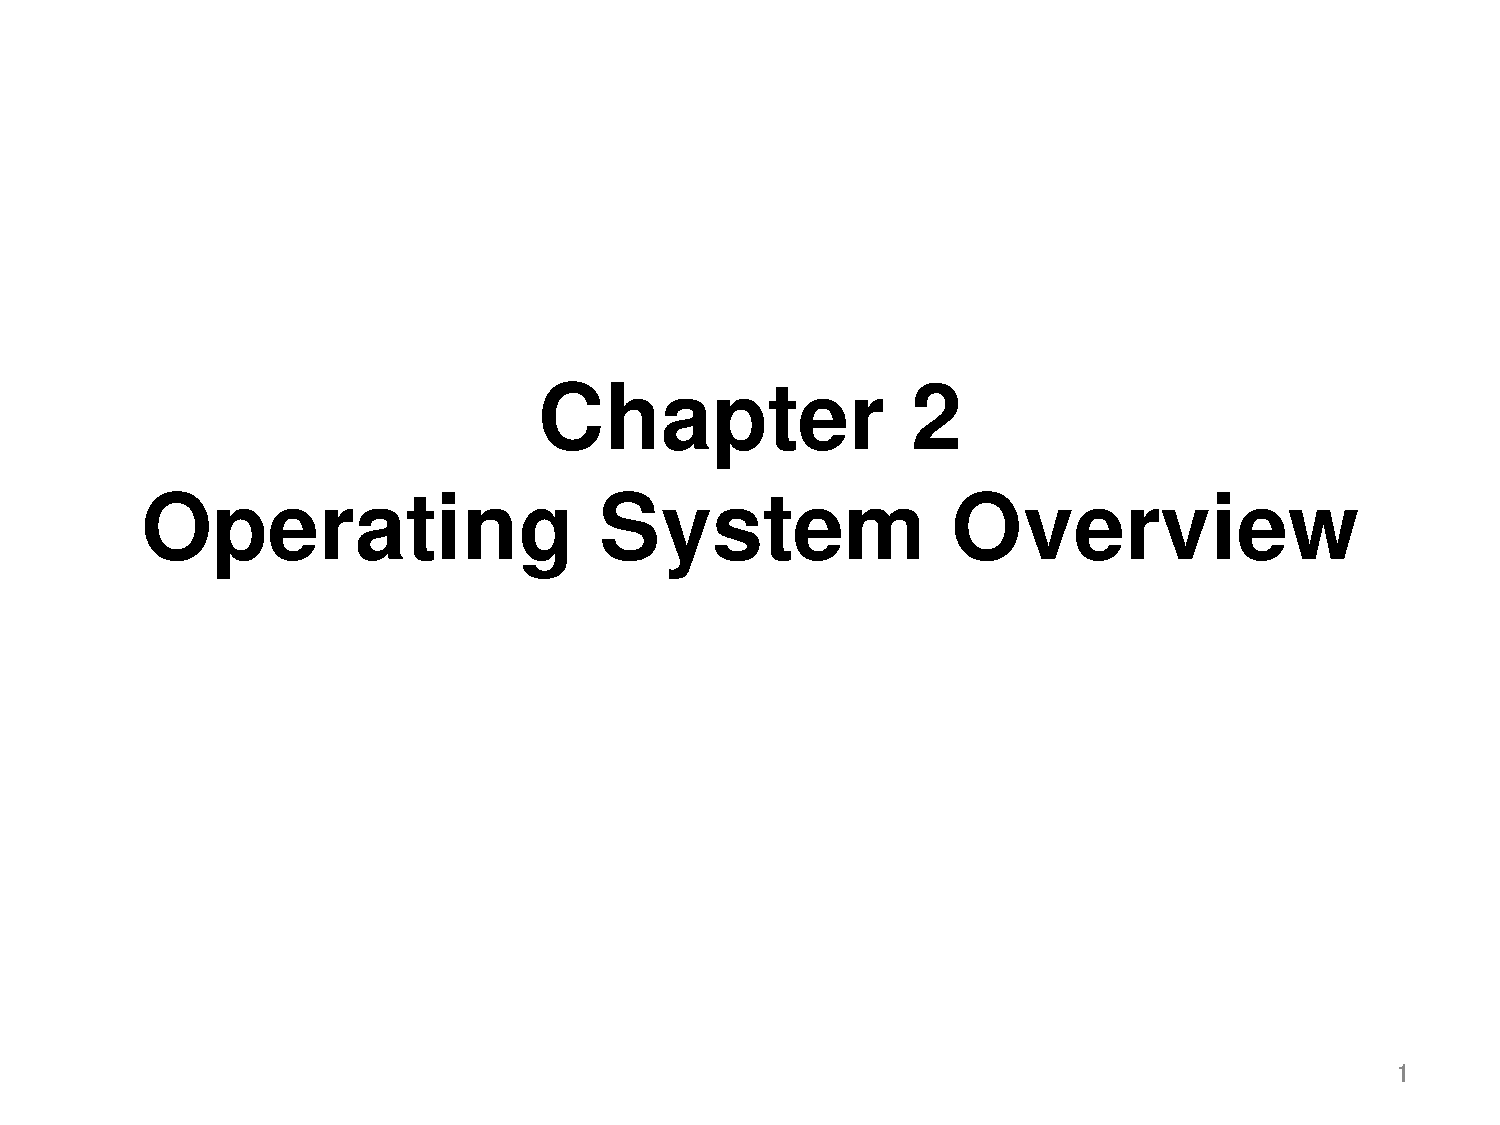
\includepdf[page=19]{03.pdf}
We really want to protect the kernal from the users, to keep them from being cheating assholes. This lead to rings of protection. Basically you have two modes, user mode (where certain instructions are strictly not allowed) and kernal mode (where we have access to protected areas). Some processors have two more modes, but almost all operating systems only use these two.
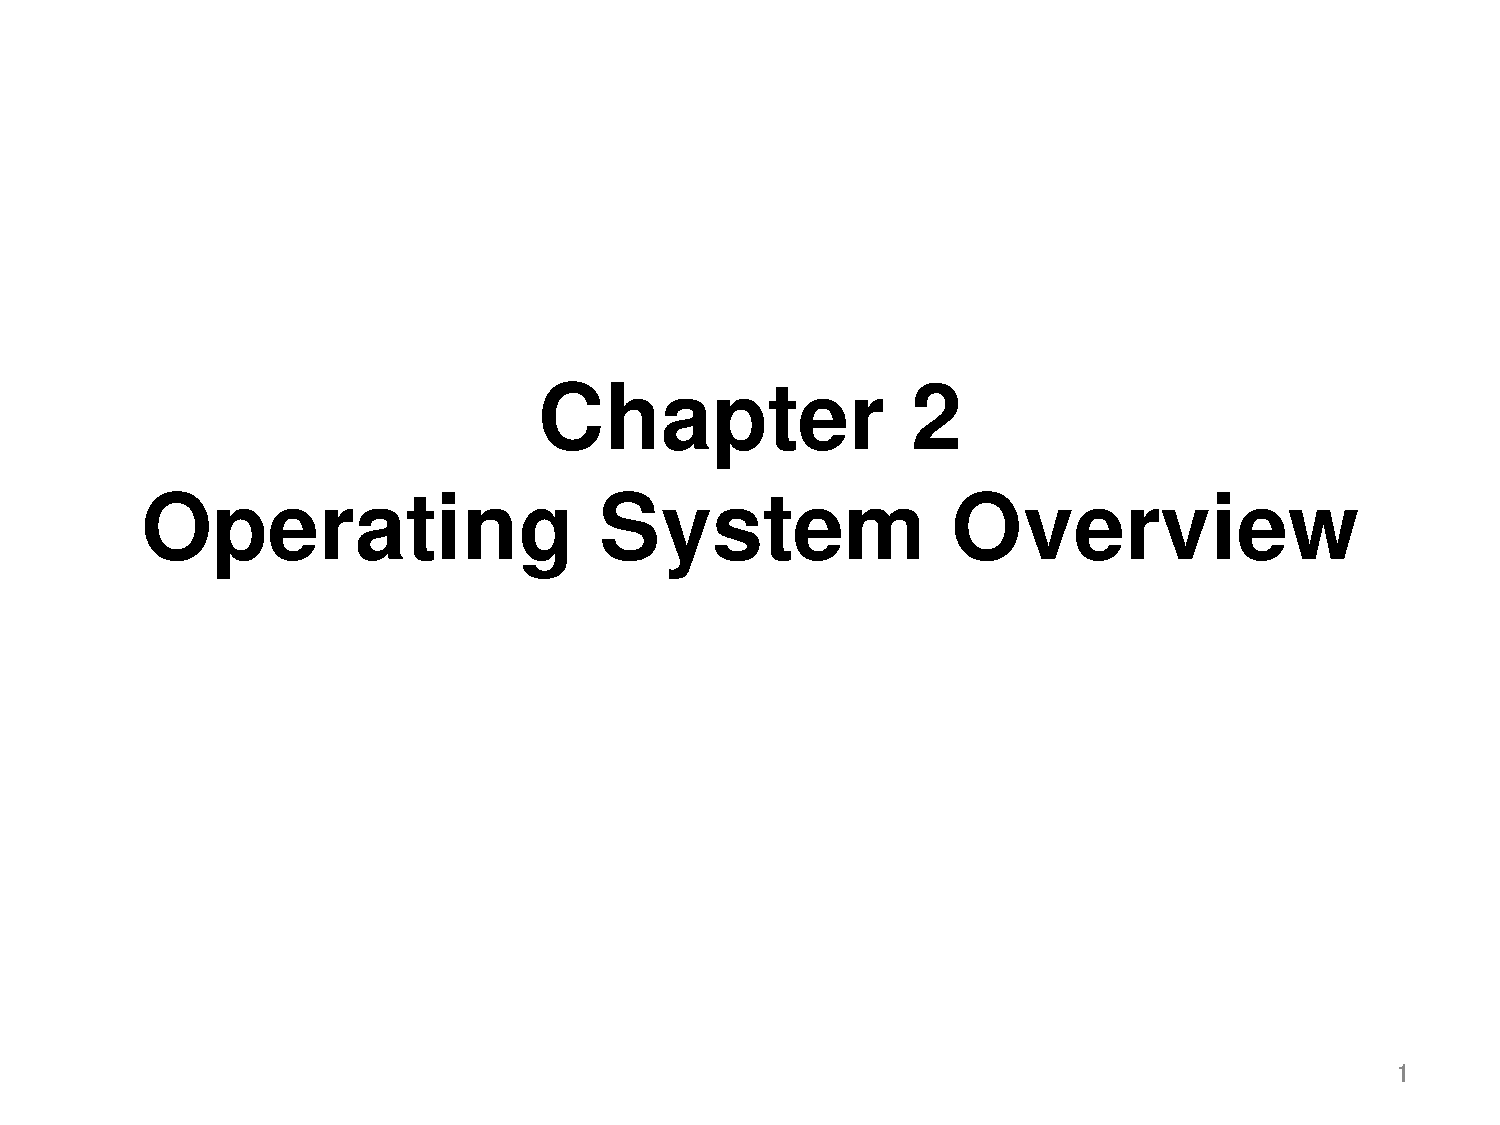
\includepdf[page=20]{03.pdf}
We care alot about CPU Utilization which is the percentage of time spent on the CPU in any function. We want this to be very high so that as little time as possible is wasted.
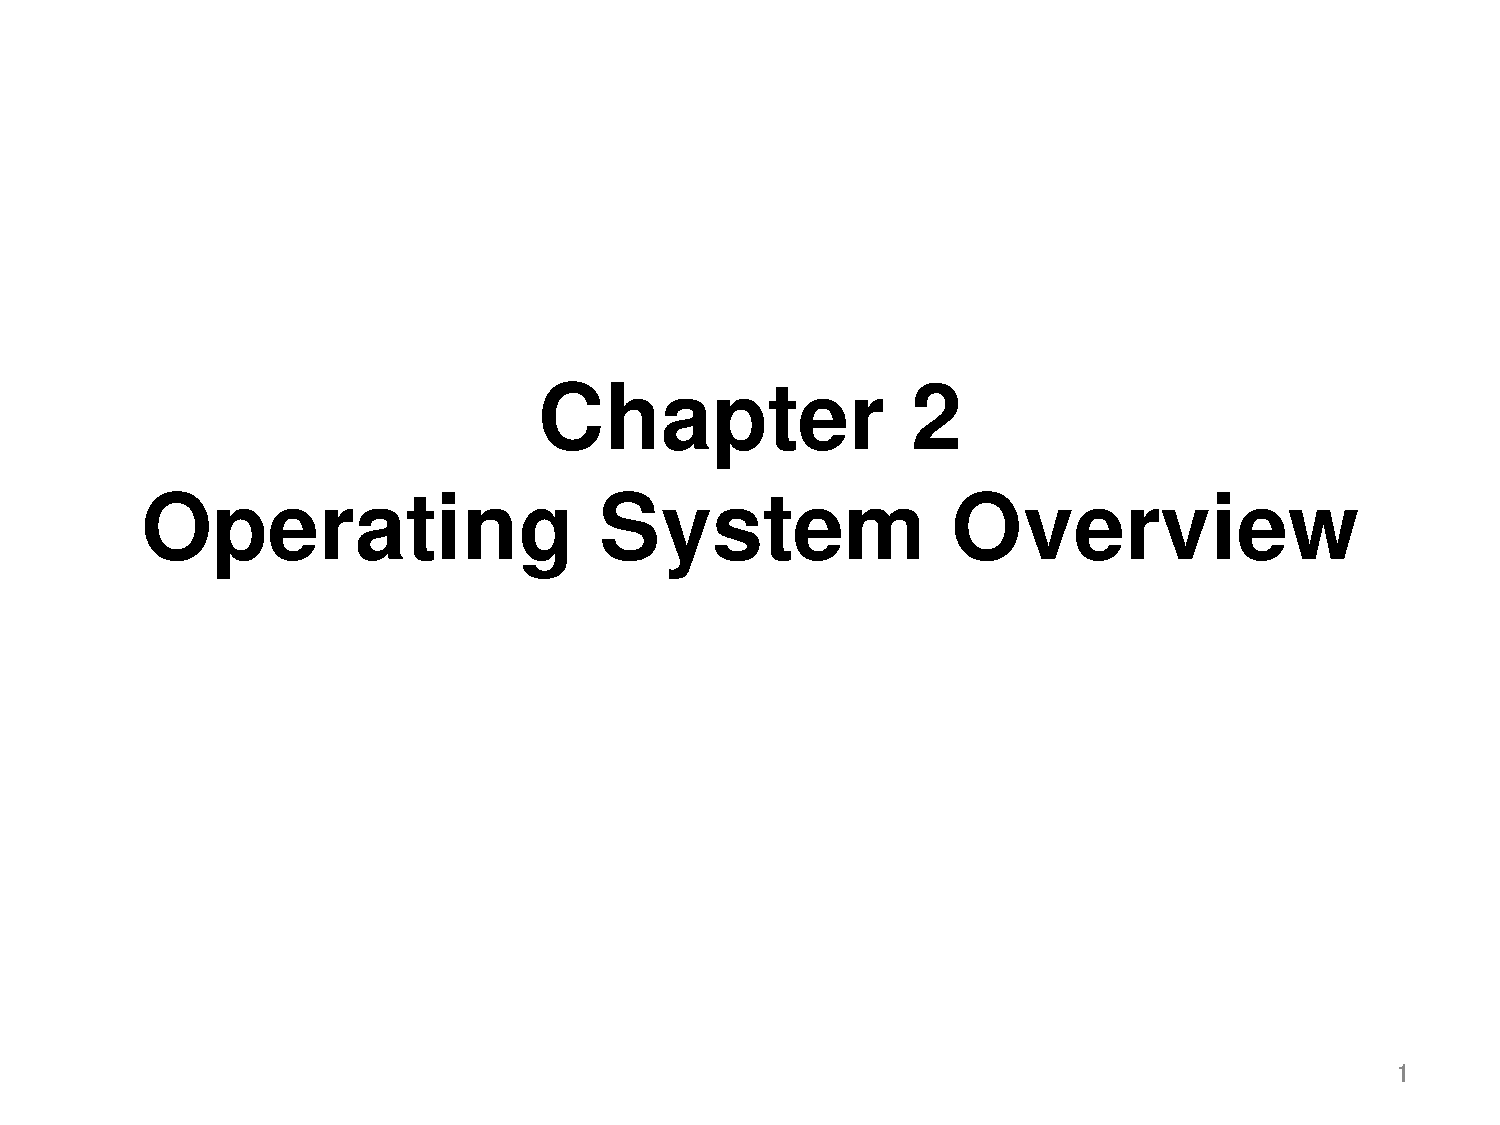
\includepdf[page=21]{03.pdf}
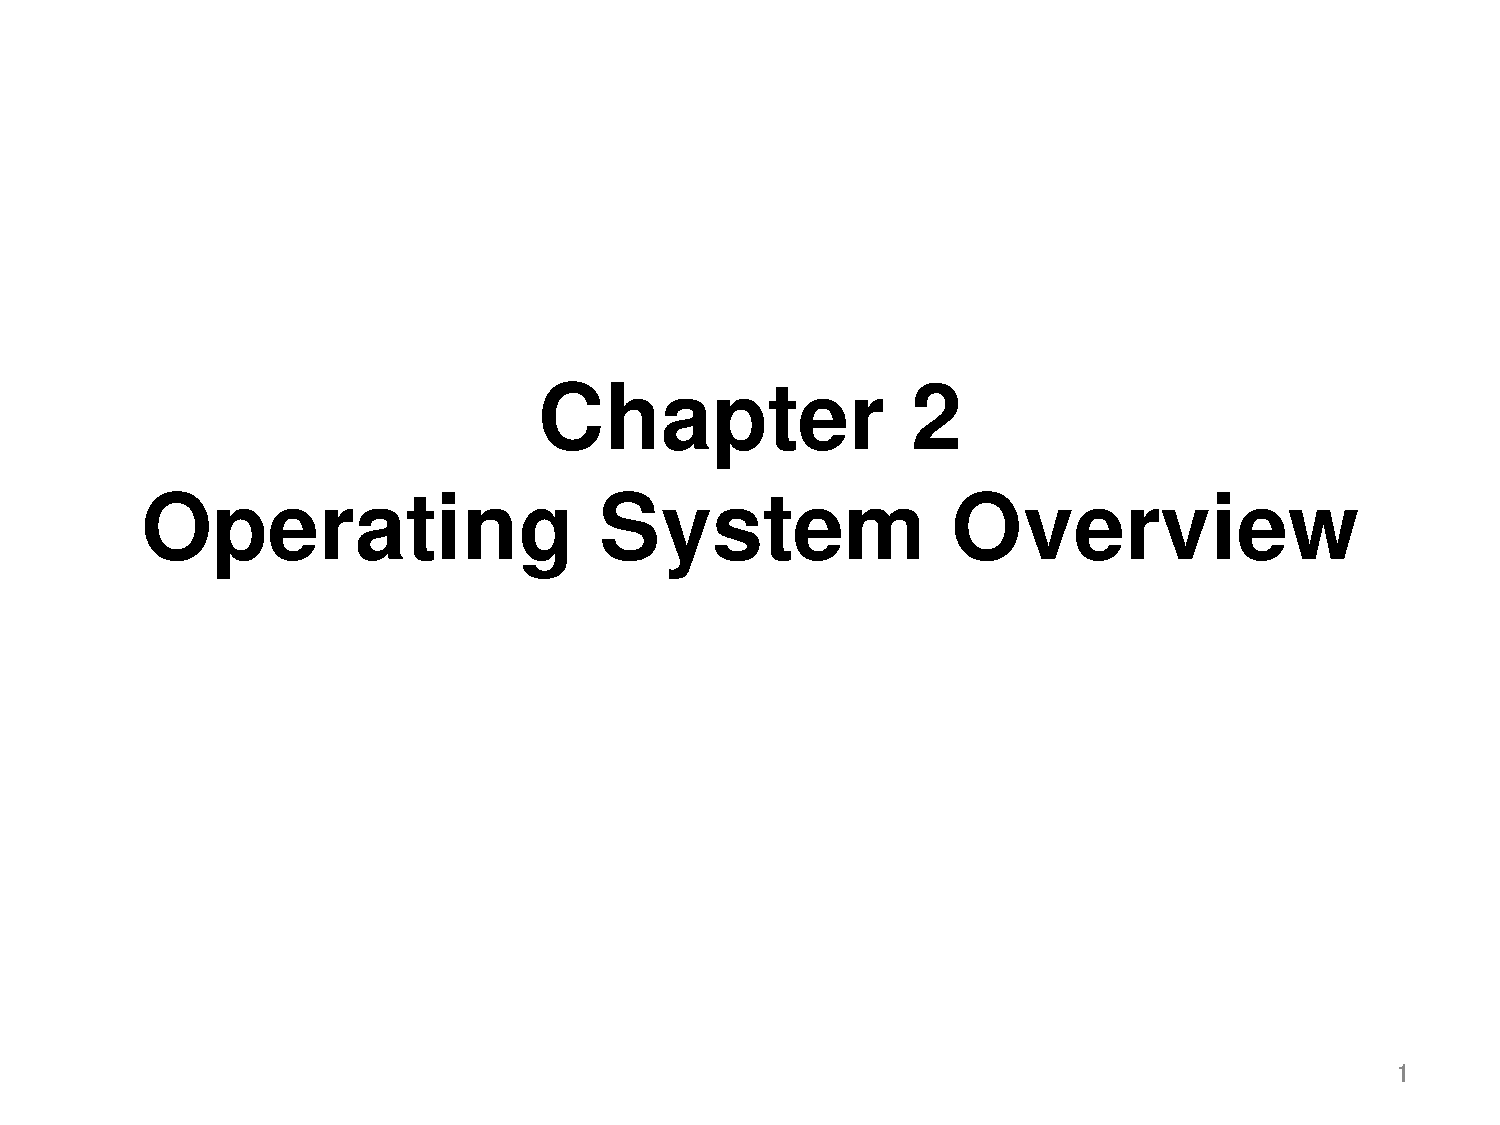
\includepdf[page=22]{03.pdf}
The most basic way to efficinize the use of the CPU is to allow multiple programs to use the CPU at the same time during the wait periods. This is the core feature of all OS. We really like this, without it most things would be impossible.
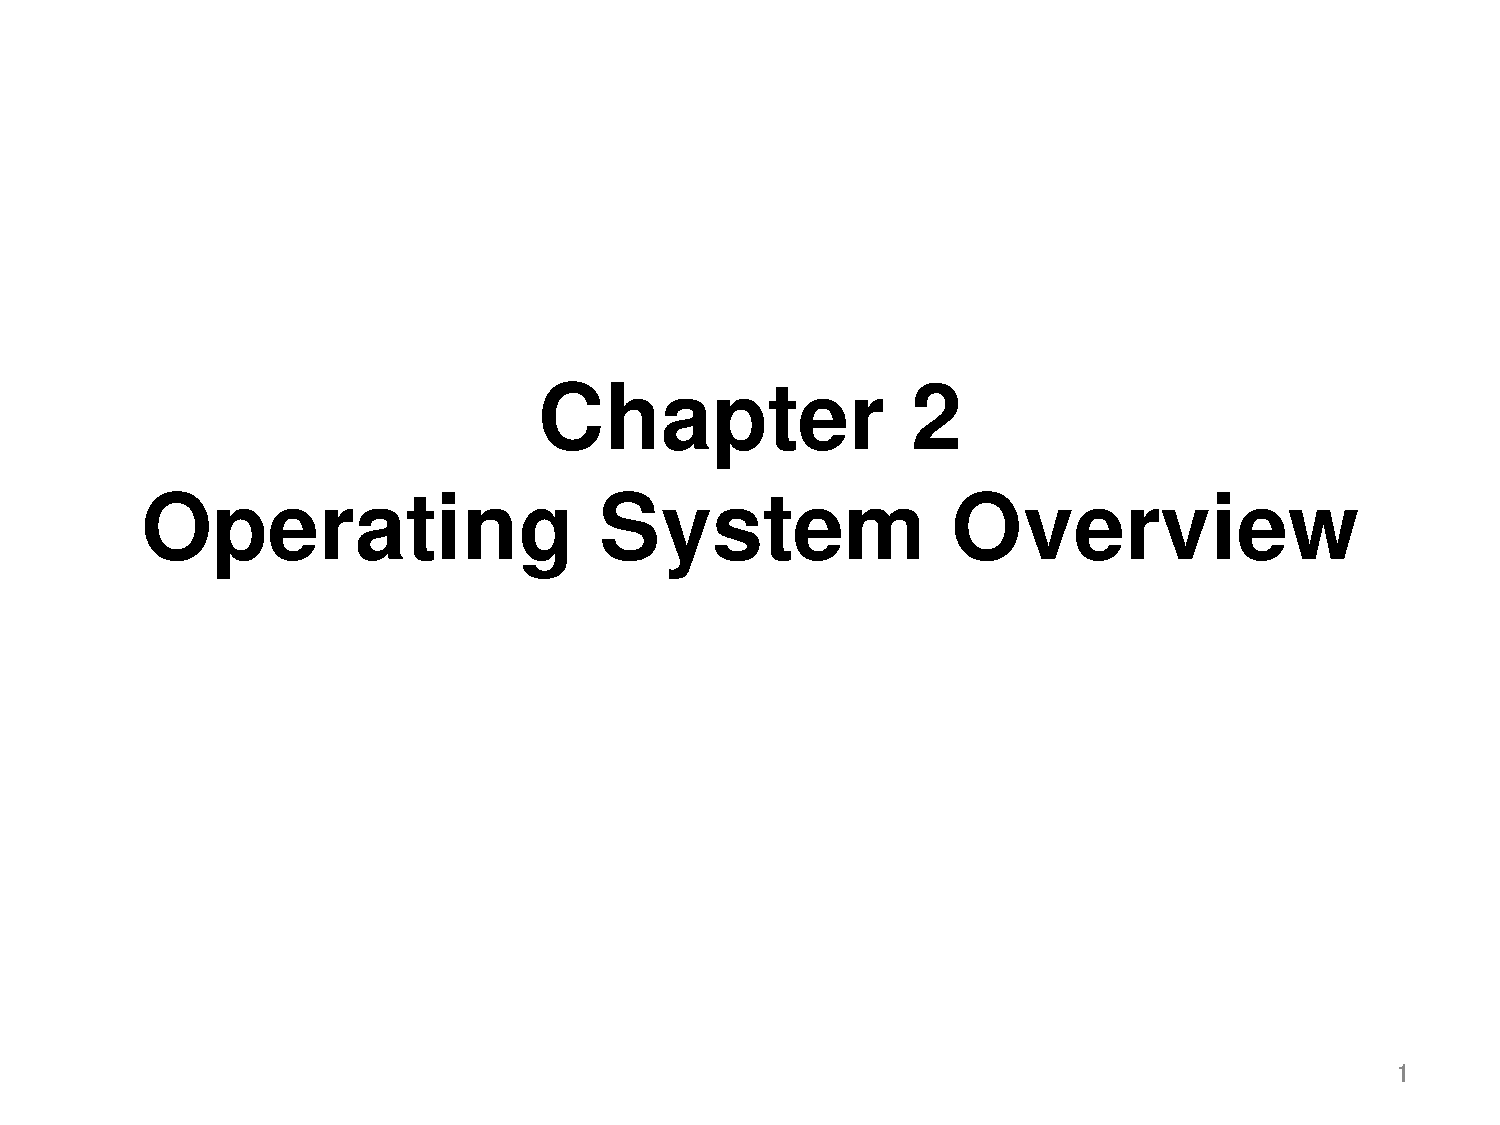
\includepdf[page=23]{03.pdf}
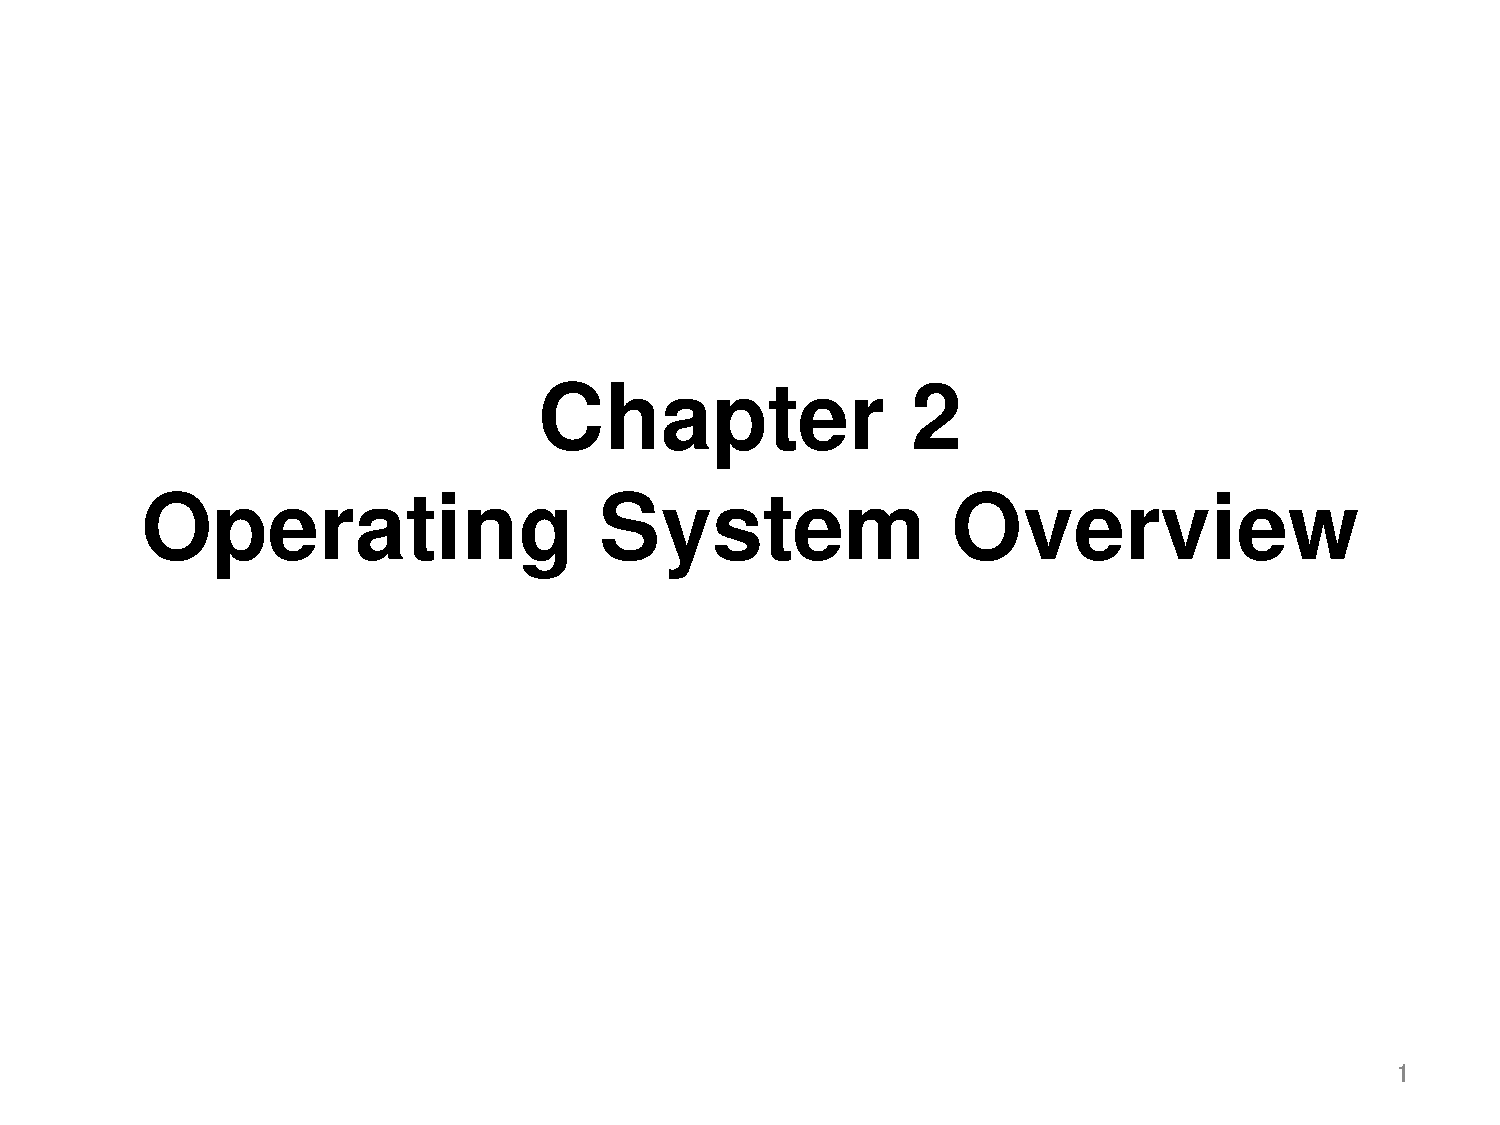
\includepdf[page=24]{03.pdf}
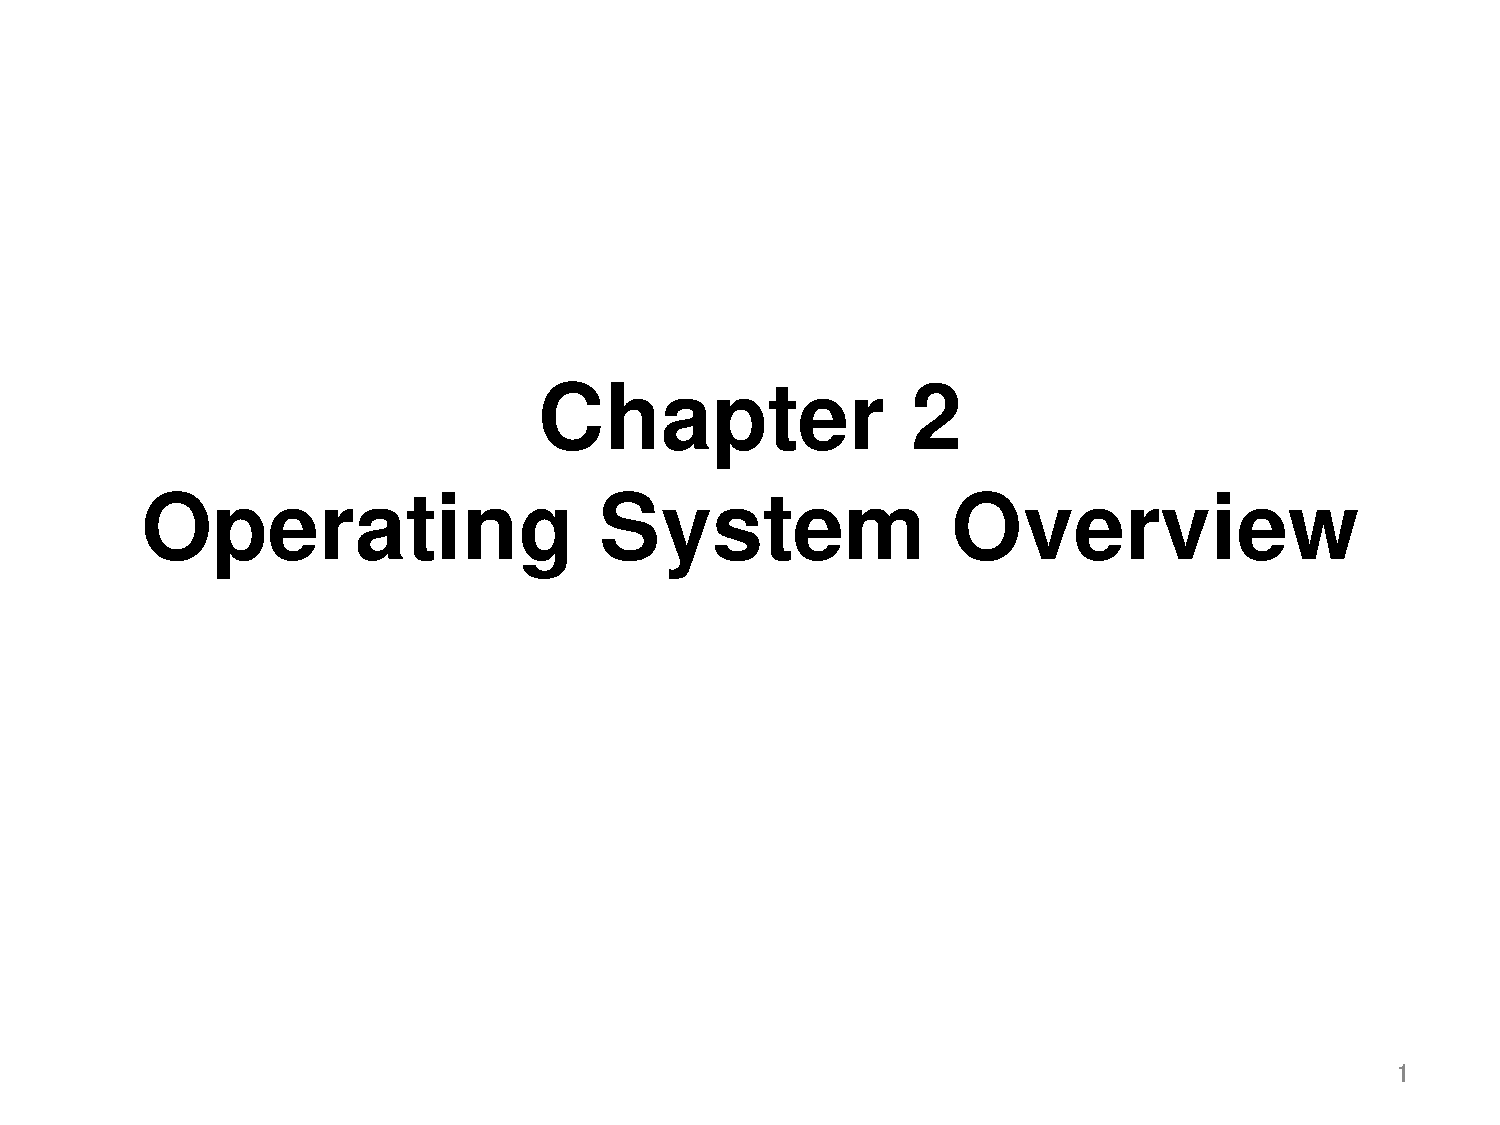
\includepdf[page=25]{03.pdf}
We can see in this example that uniprocessing would suck balls to do this (30 min). If we use multiprocessing we can cut this down to the shortest period of time.
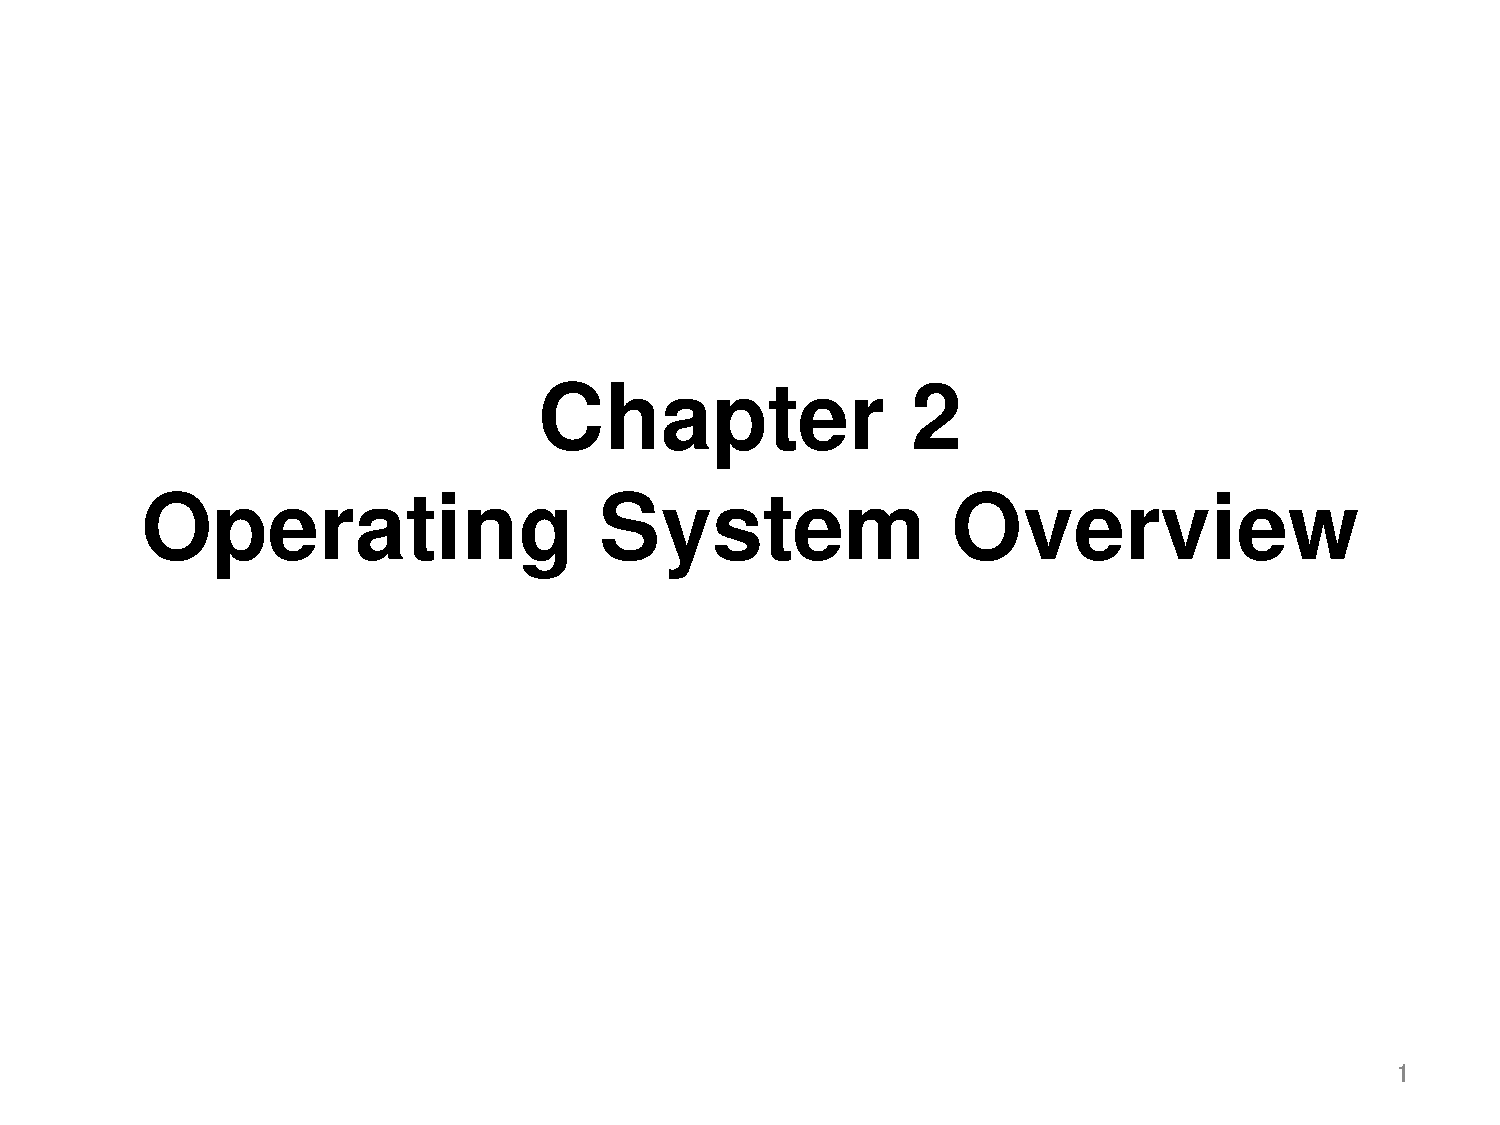
\includepdf[page=26]{03.pdf}
By running multiple things at once we make everything way more efficient.
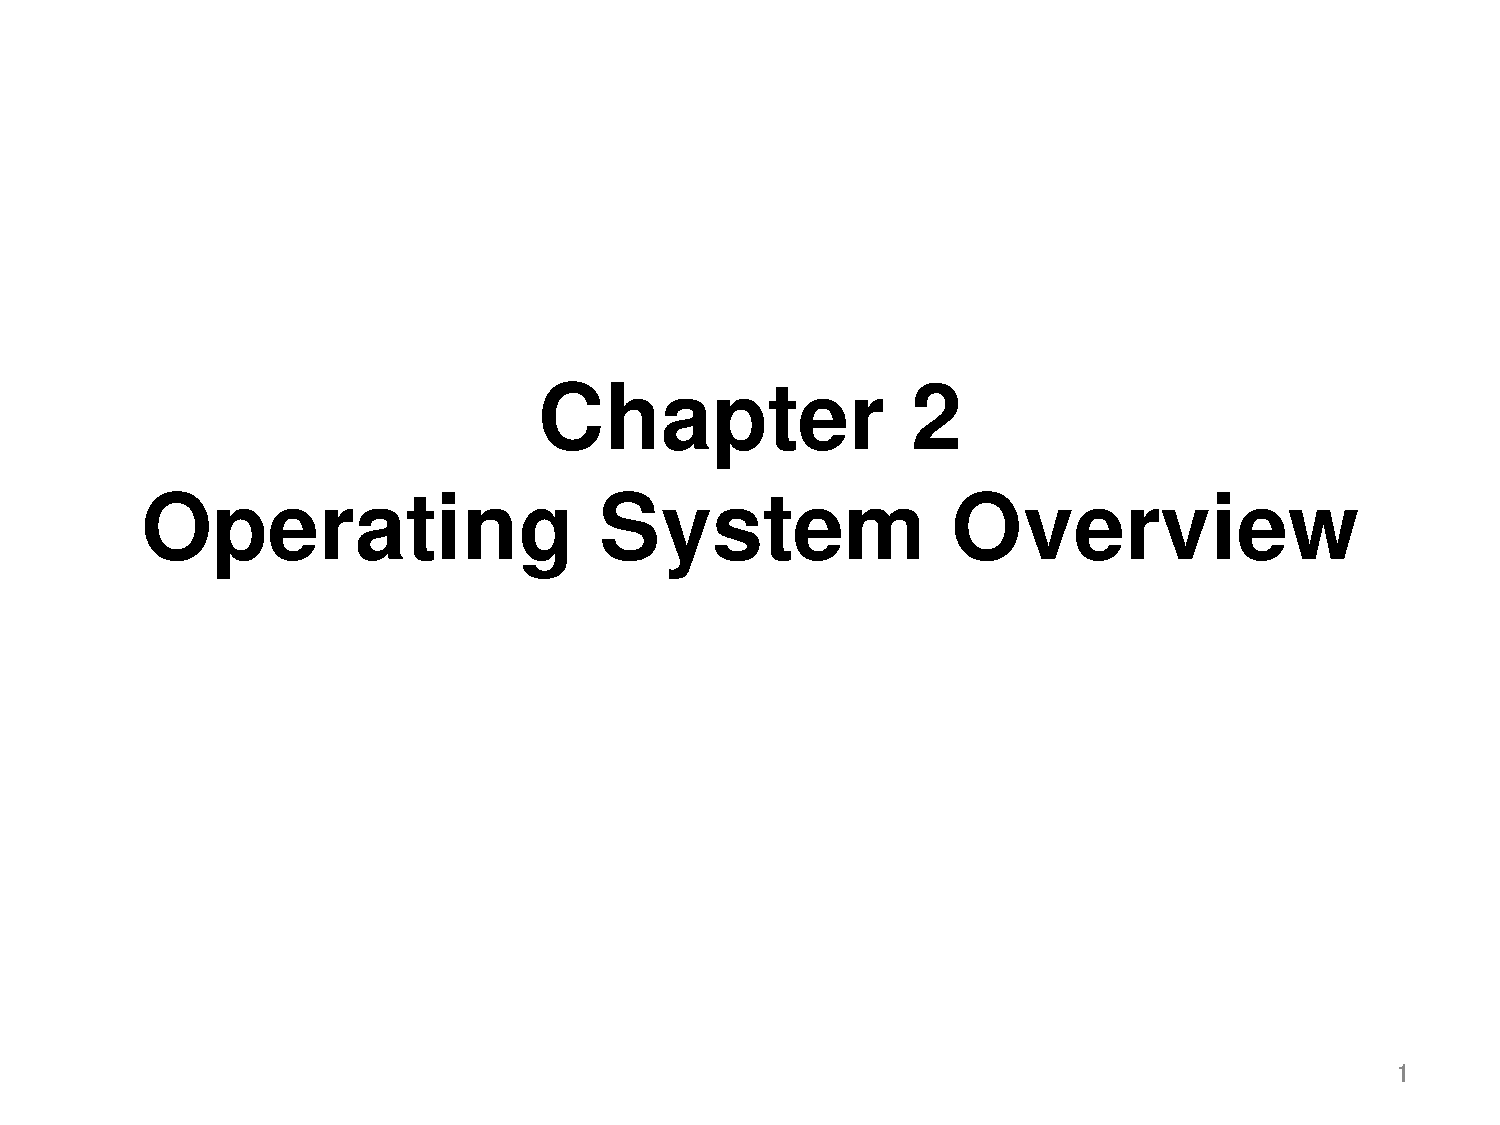
\includepdf[page=27]{03.pdf}
Batch programming doesnt help when a program needs user interaction.
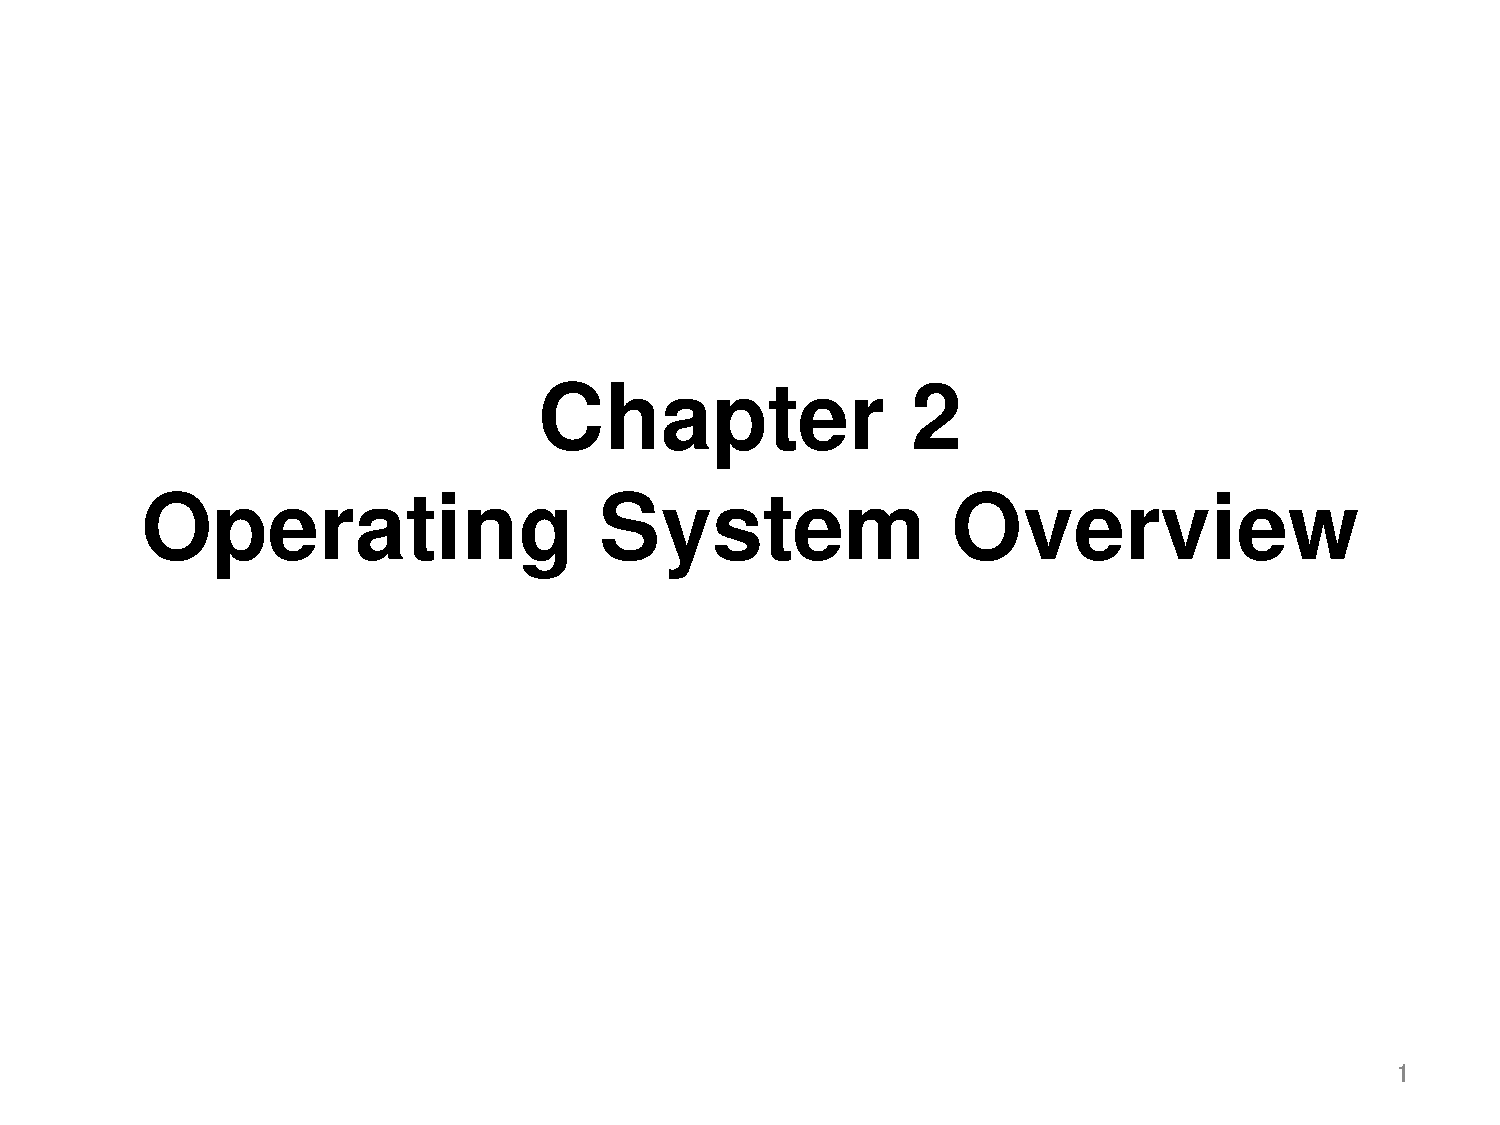
\includepdf[page=28]{03.pdf}
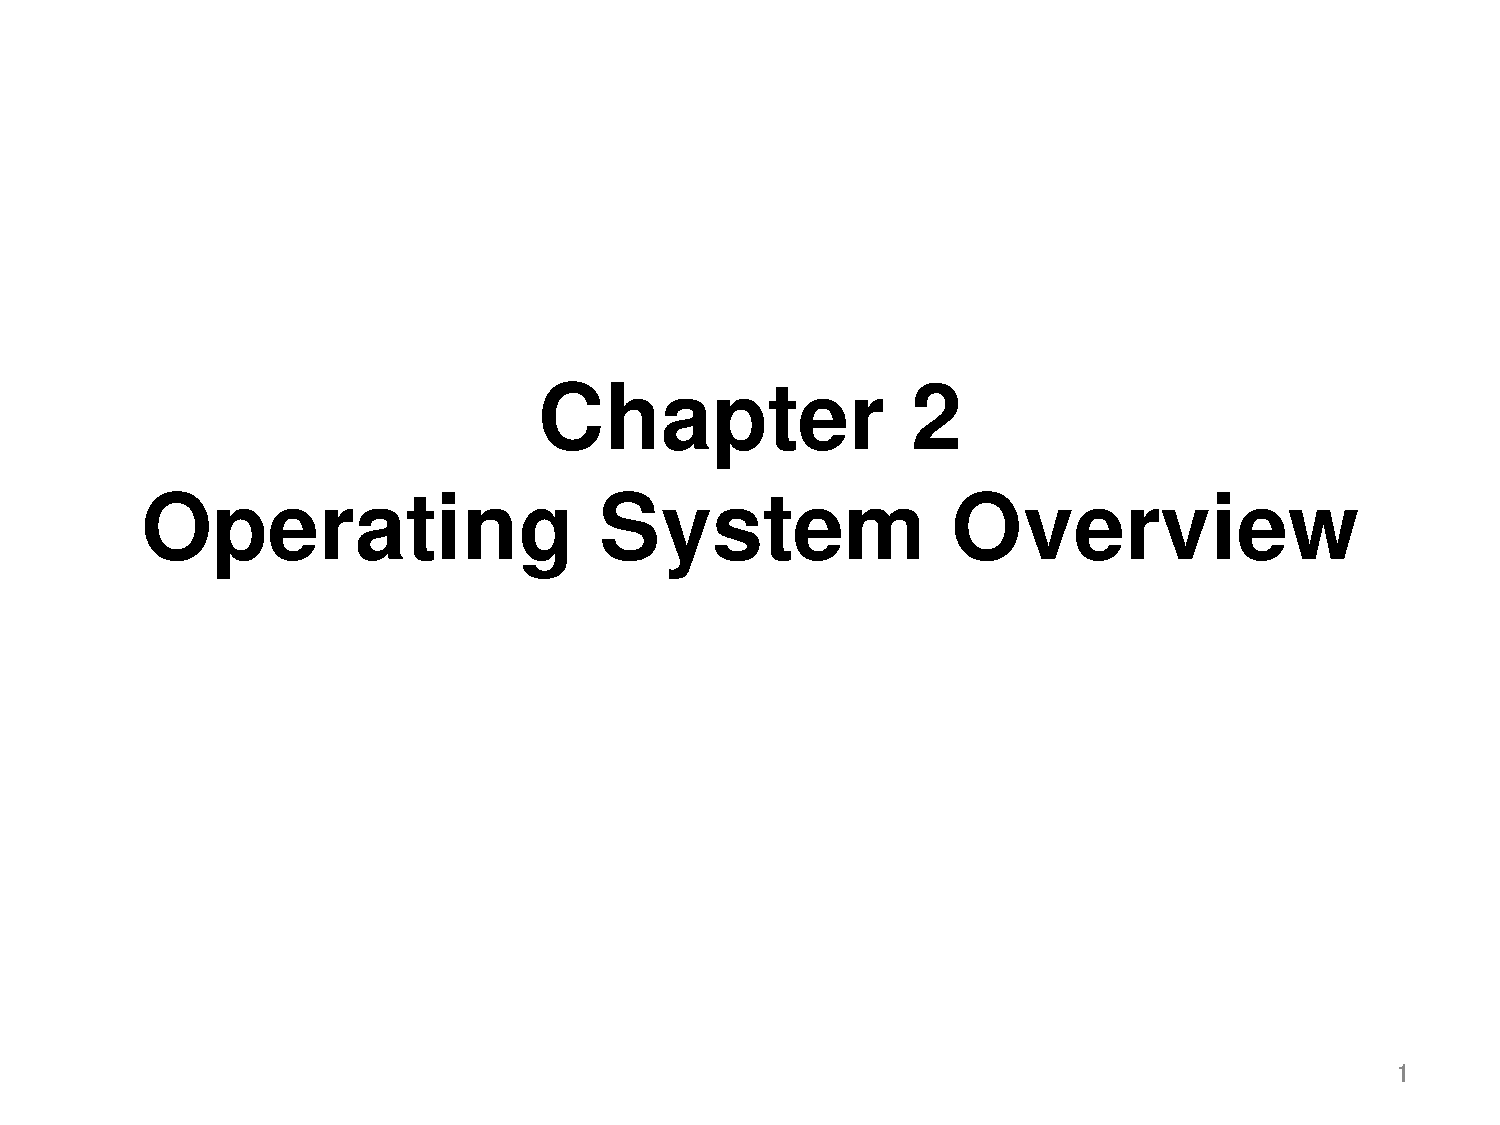
\includepdf[page=29]{03.pdf}
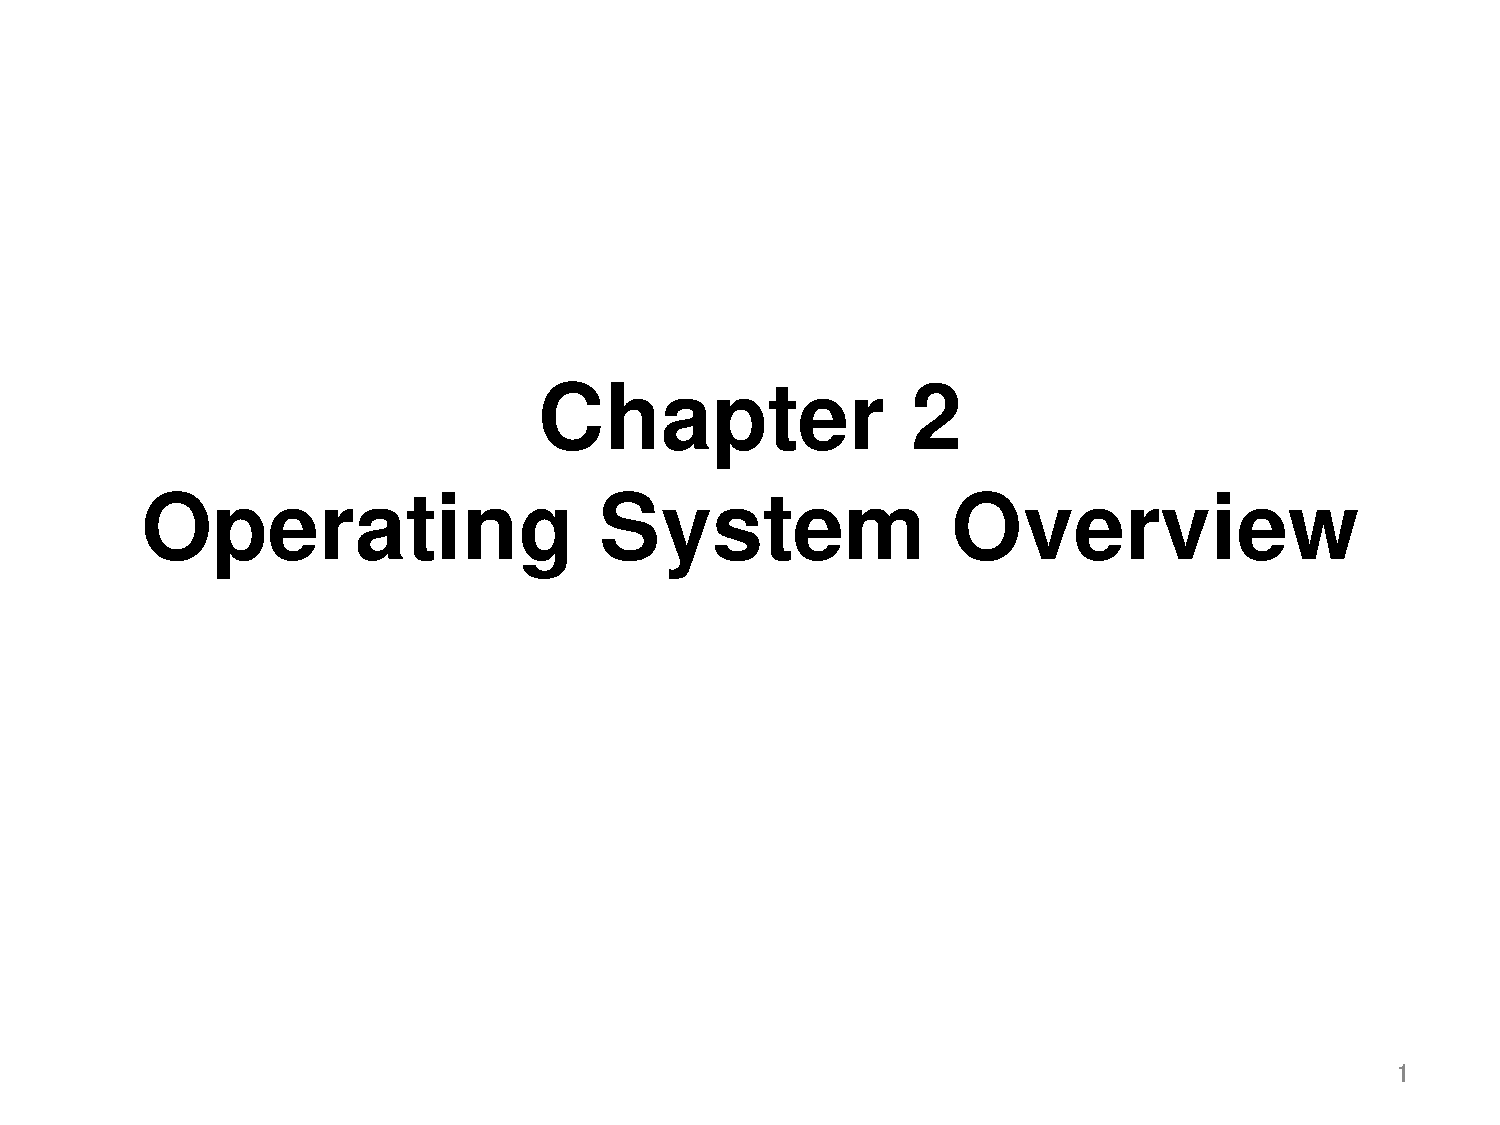
\includepdf[page=30]{03.pdf}
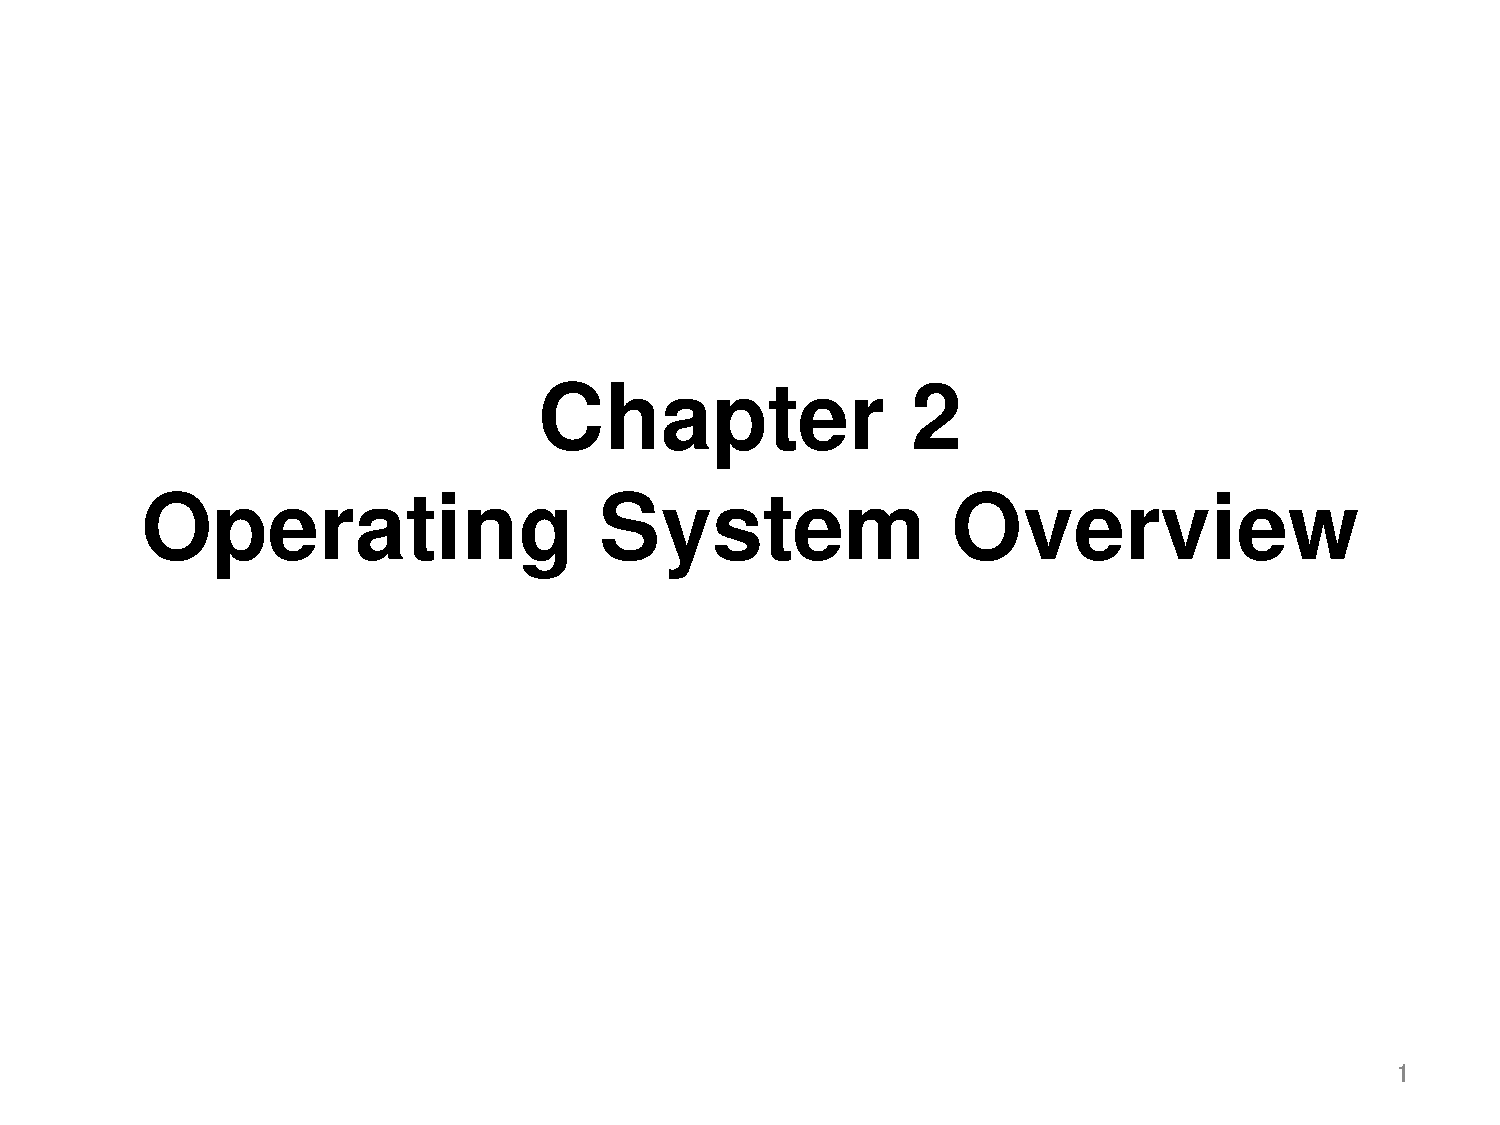
\includepdf[page=31]{03.pdf}
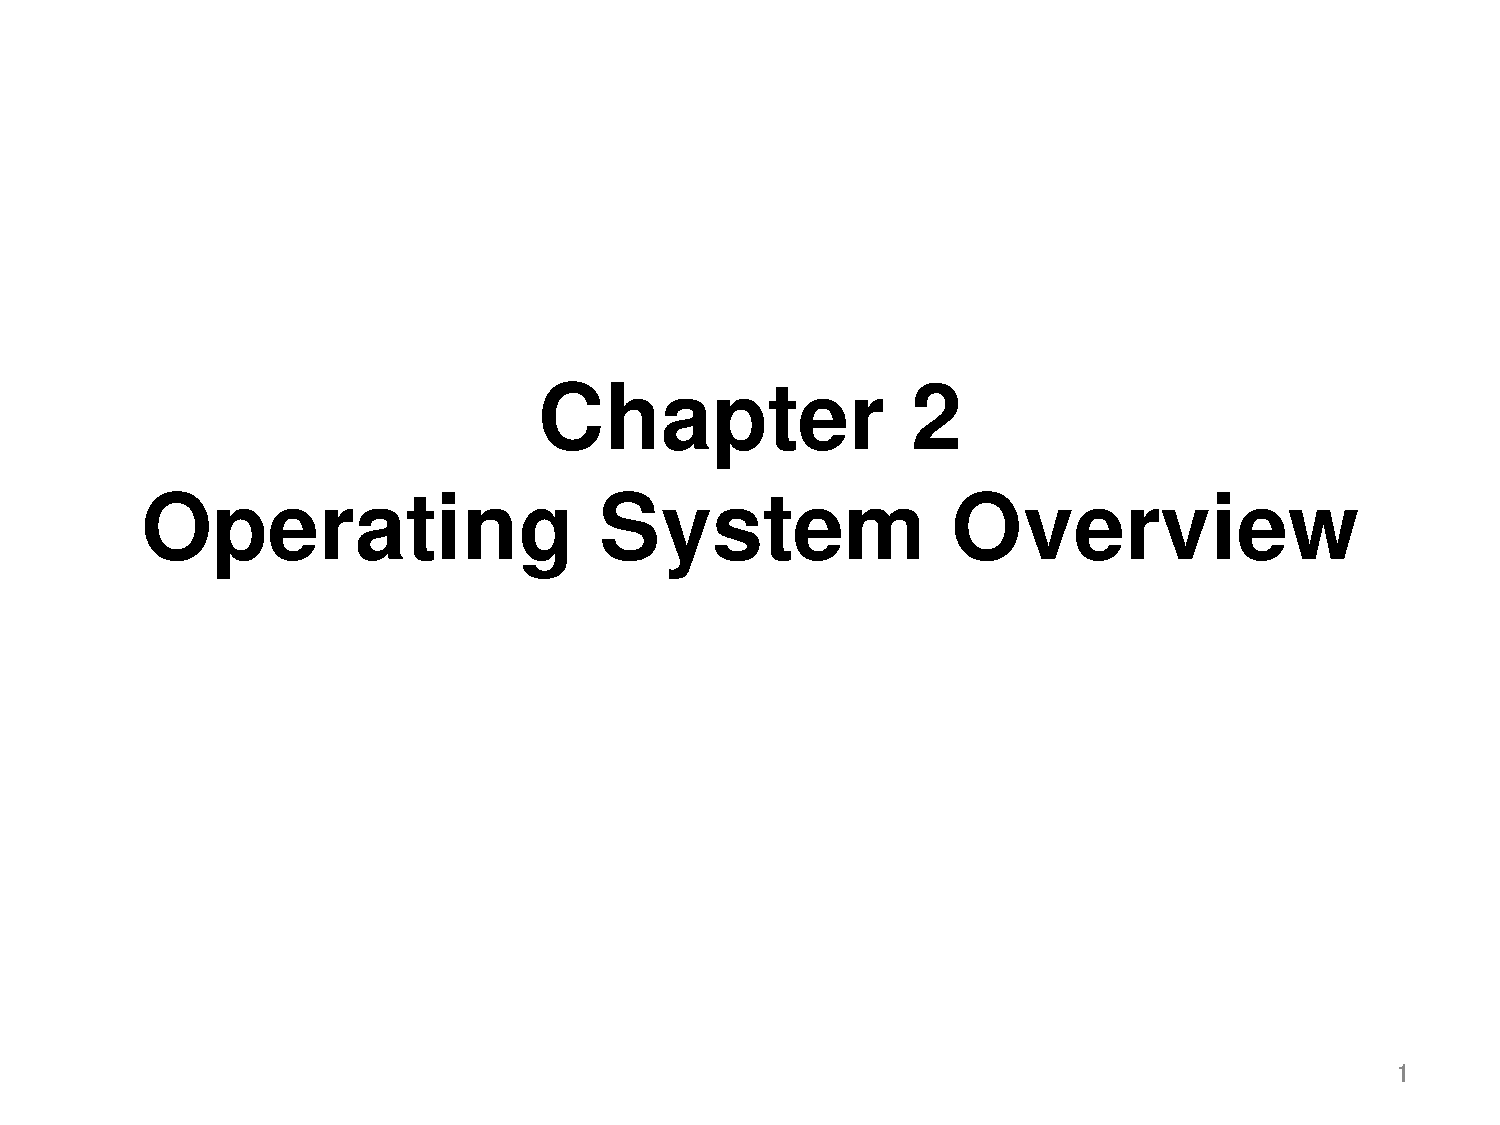
\includepdf[page=32]{03.pdf}
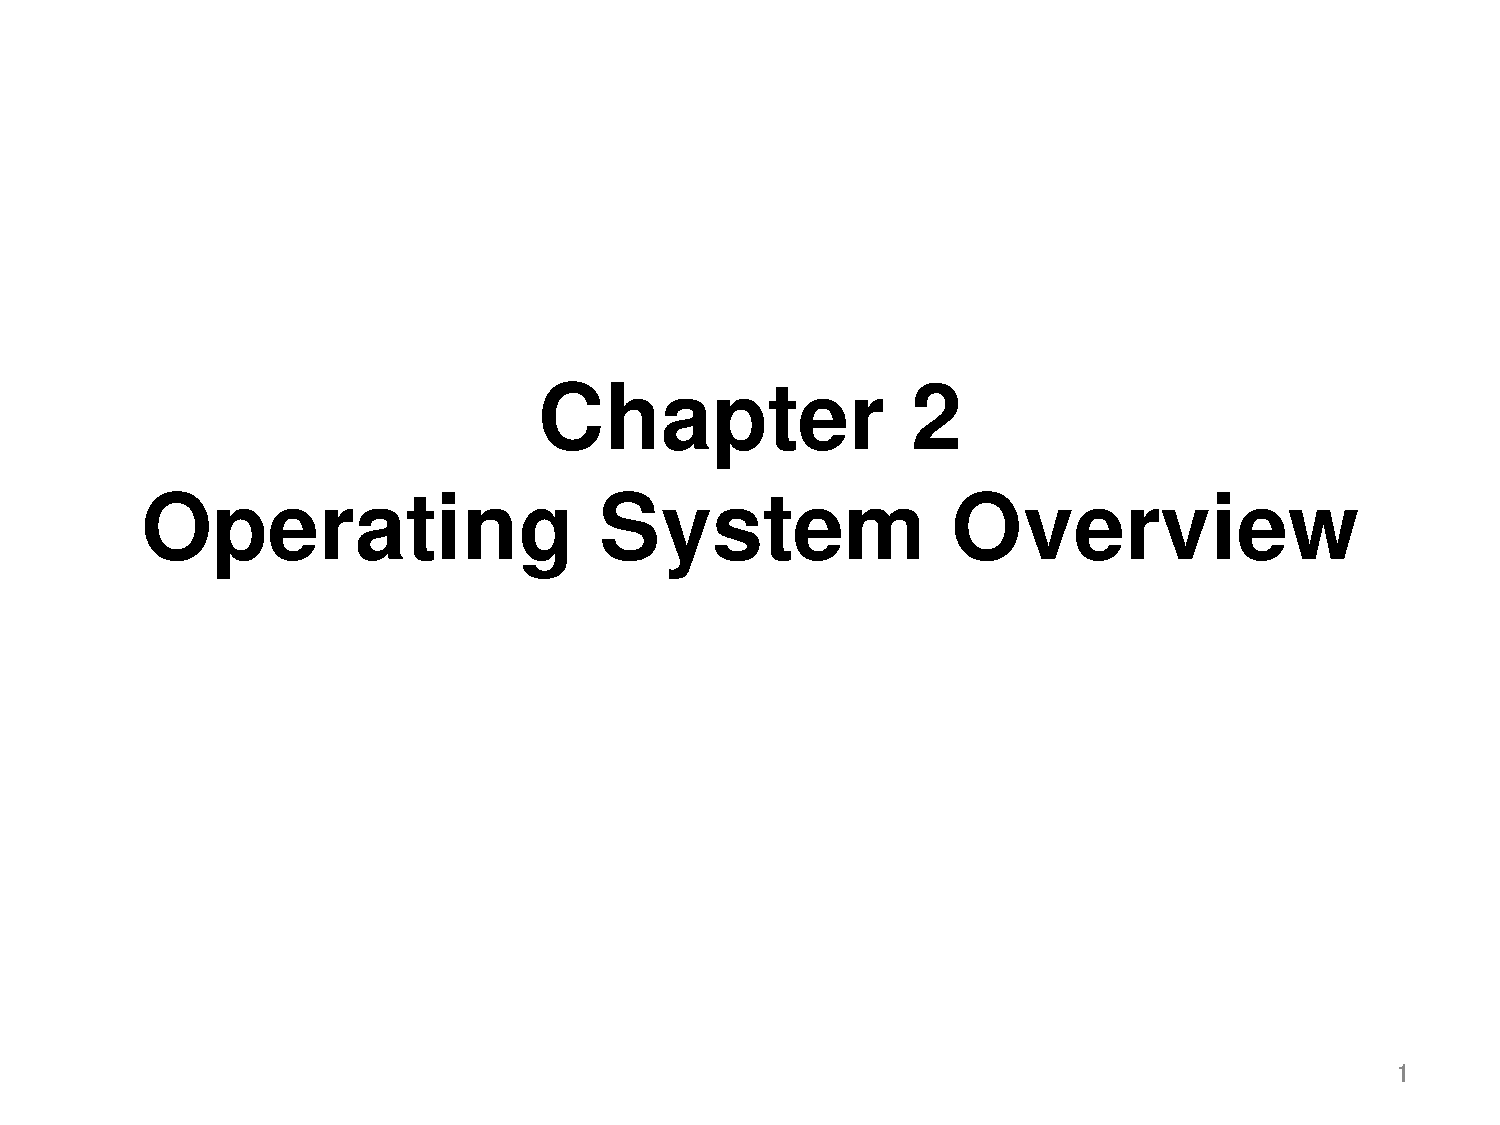
\includepdf[page=33]{03.pdf}
The most basic means of memory protection is to identify the set the chunk of memory allowed to that program restrict access outside of that.
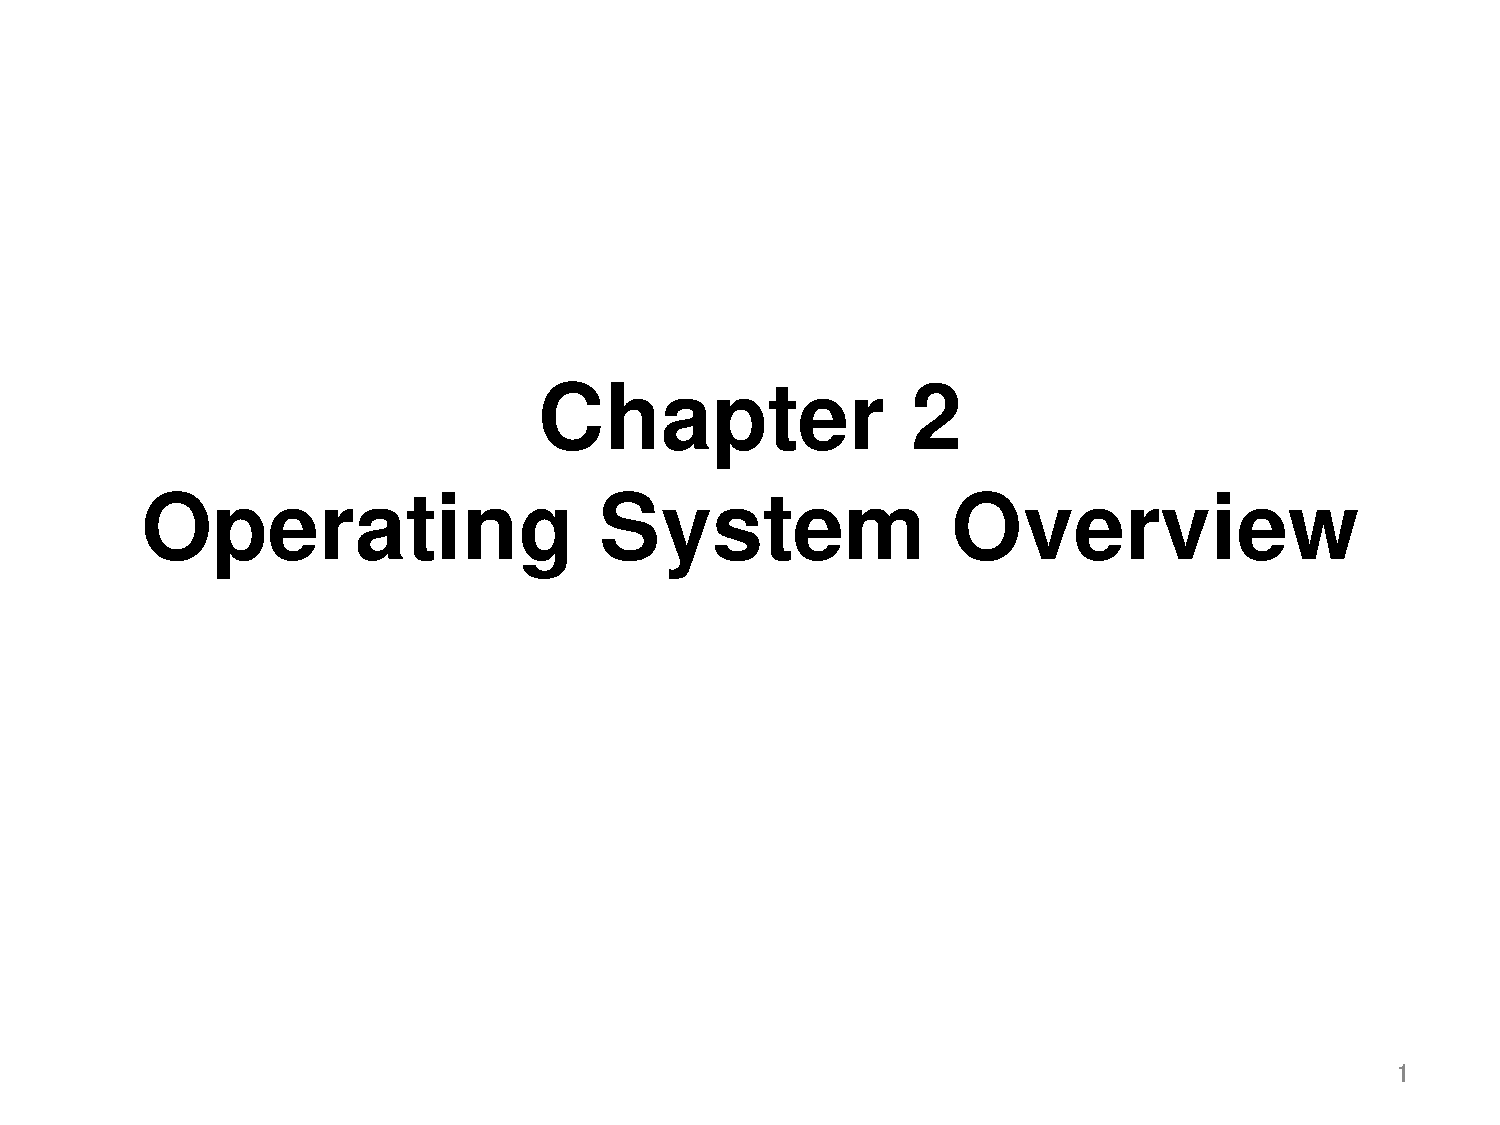
\includepdf[page=34]{03.pdf}
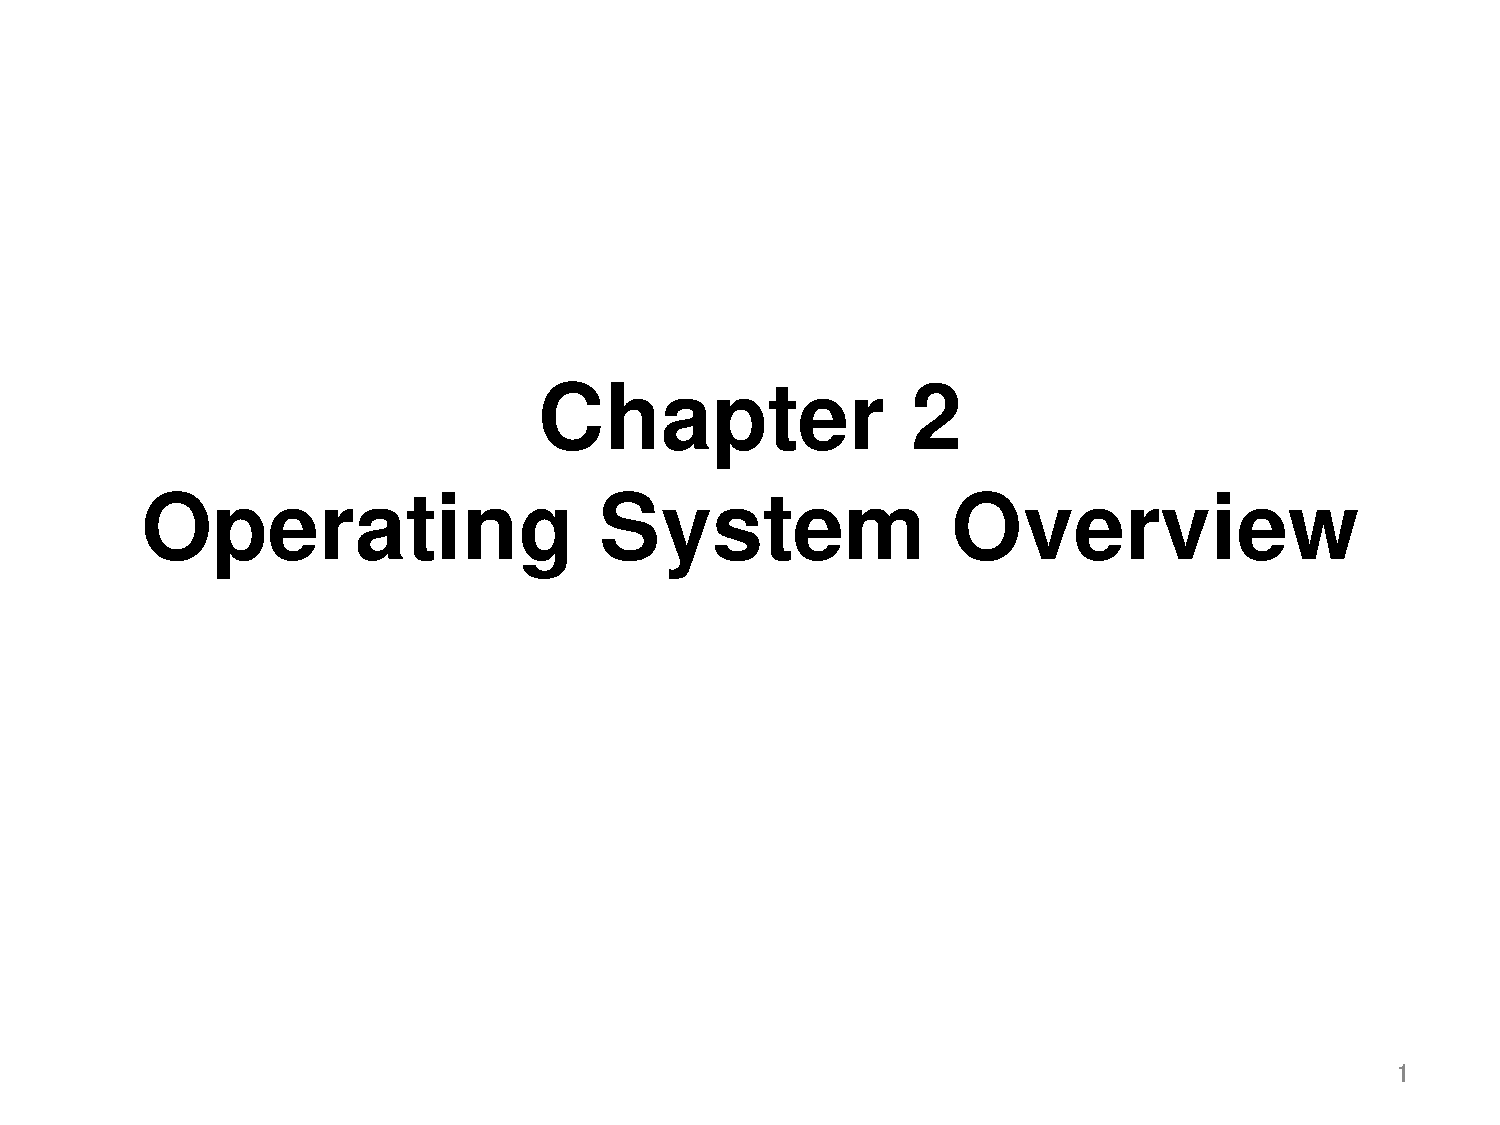
\includepdf[page=35]{03.pdf}
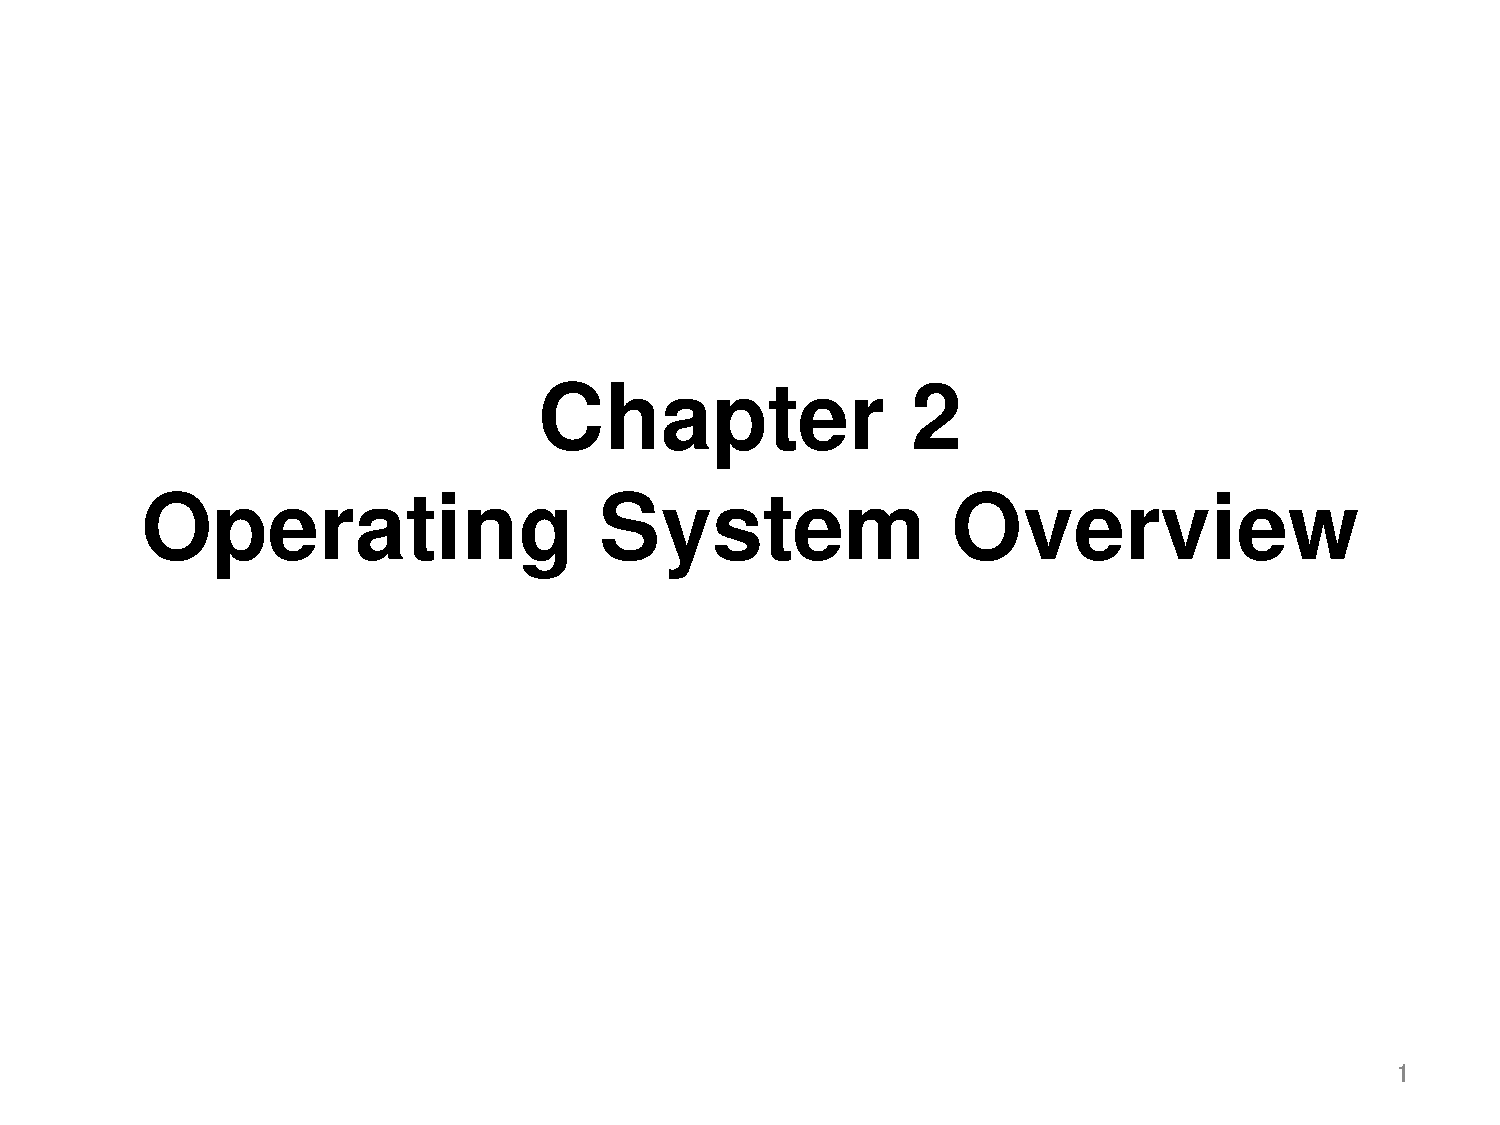
\includepdf[page=36]{03.pdf}
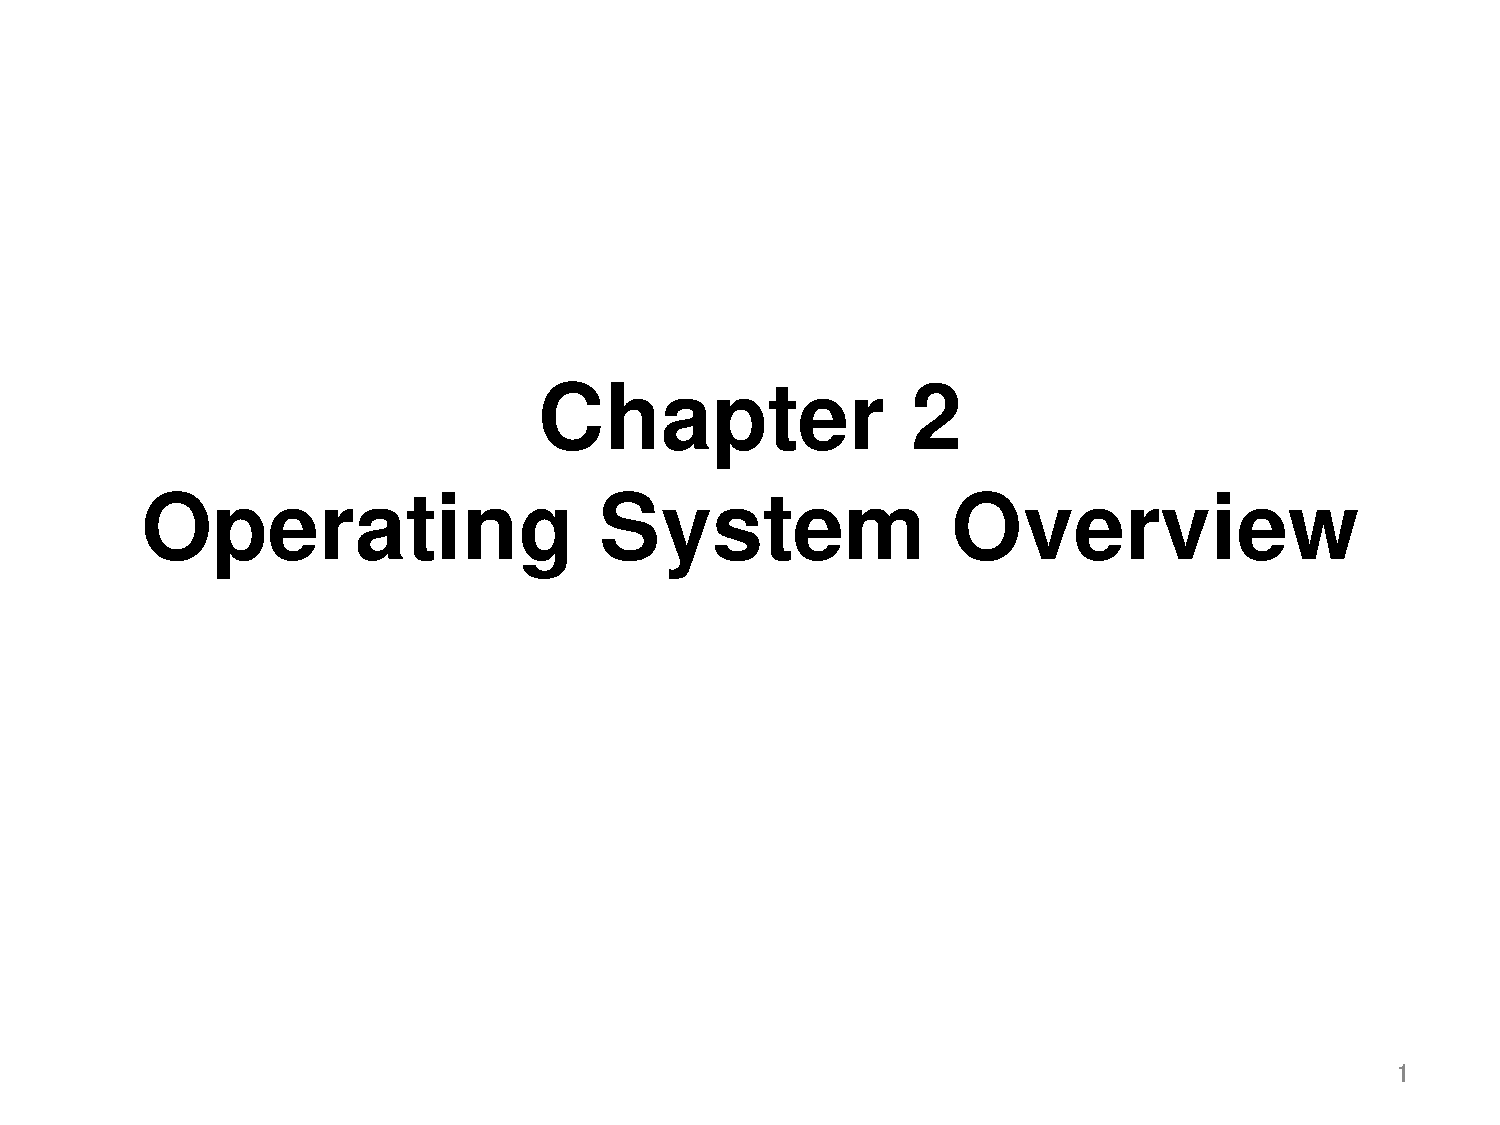
\includepdf[page=37]{03.pdf}
This allows us to game the program into thinking that it has more memory than it does. Every address that we use is just the number of a page (which is just a chunk of memory).
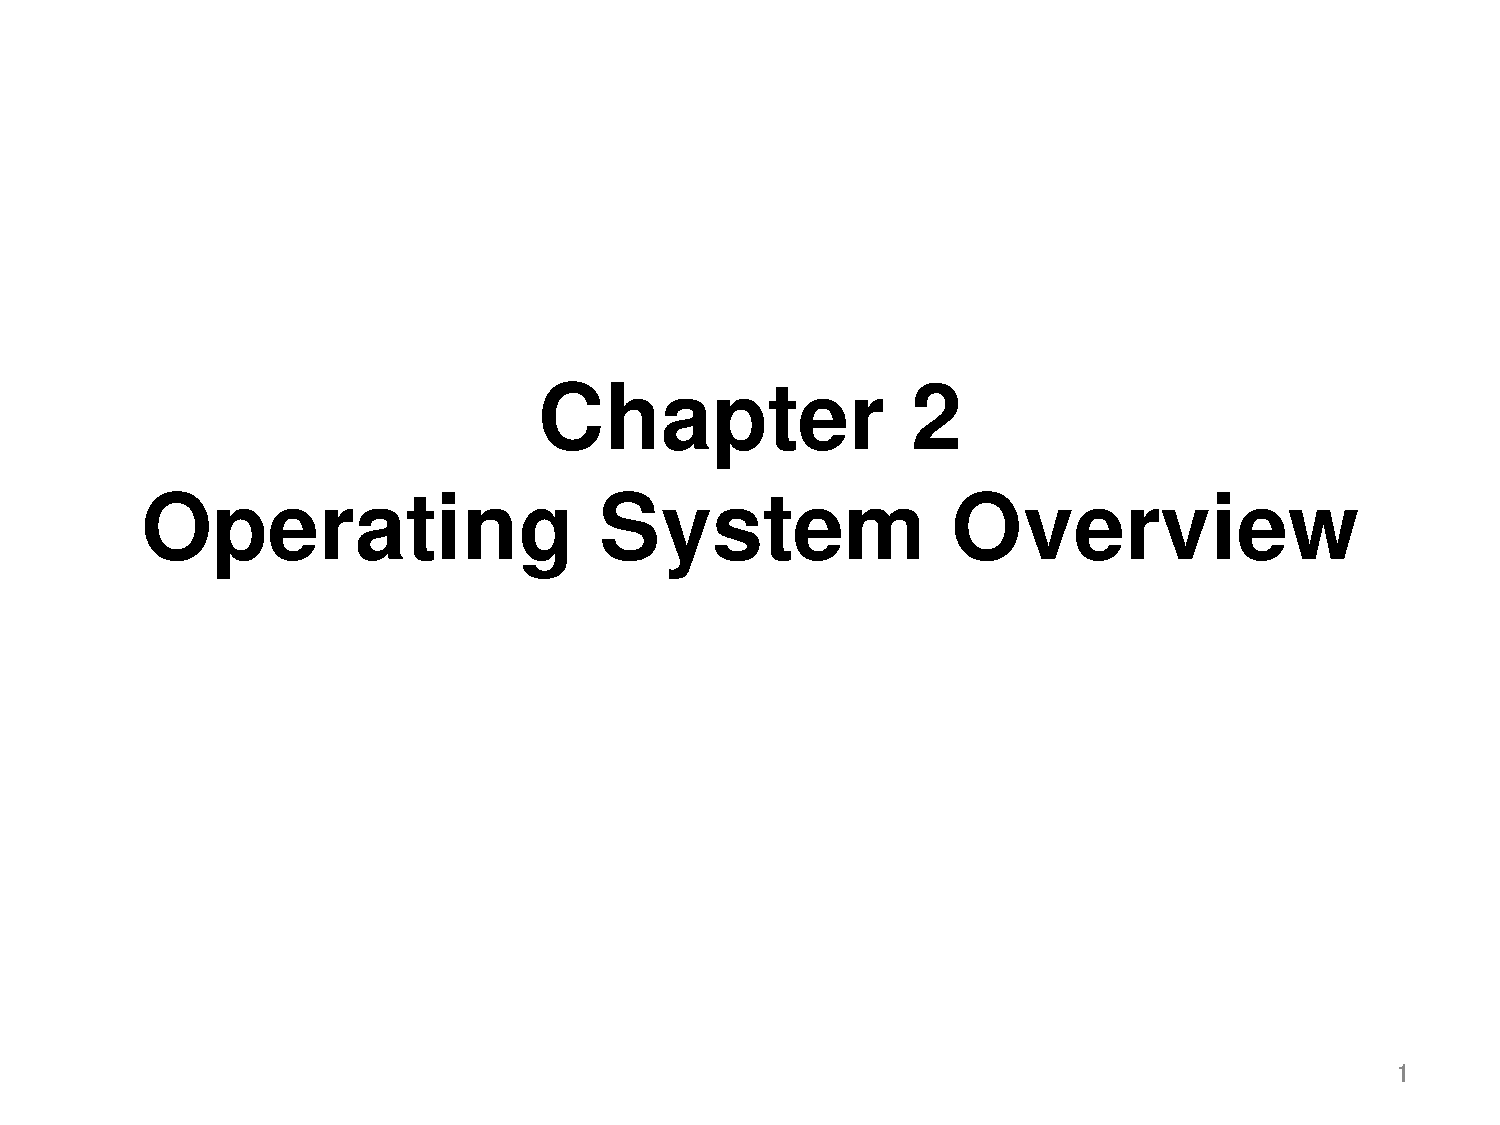
\includepdf[page=38]{03.pdf}
We organize our virtual memory system into fixed size blocks. Say we have 5 blocks of memory, we let the A have slot 0-3 and be have slots 0-4. This makes it seem like we have 4+5=9 chunks of memory, but some chunks of memory are being mapped to twice. Each program can only execute when PC for each program is stored in memory. We have some peice of hardware that maps chunks in the program chunks to the correct chunks of memory in the main memory which is a finite resource.
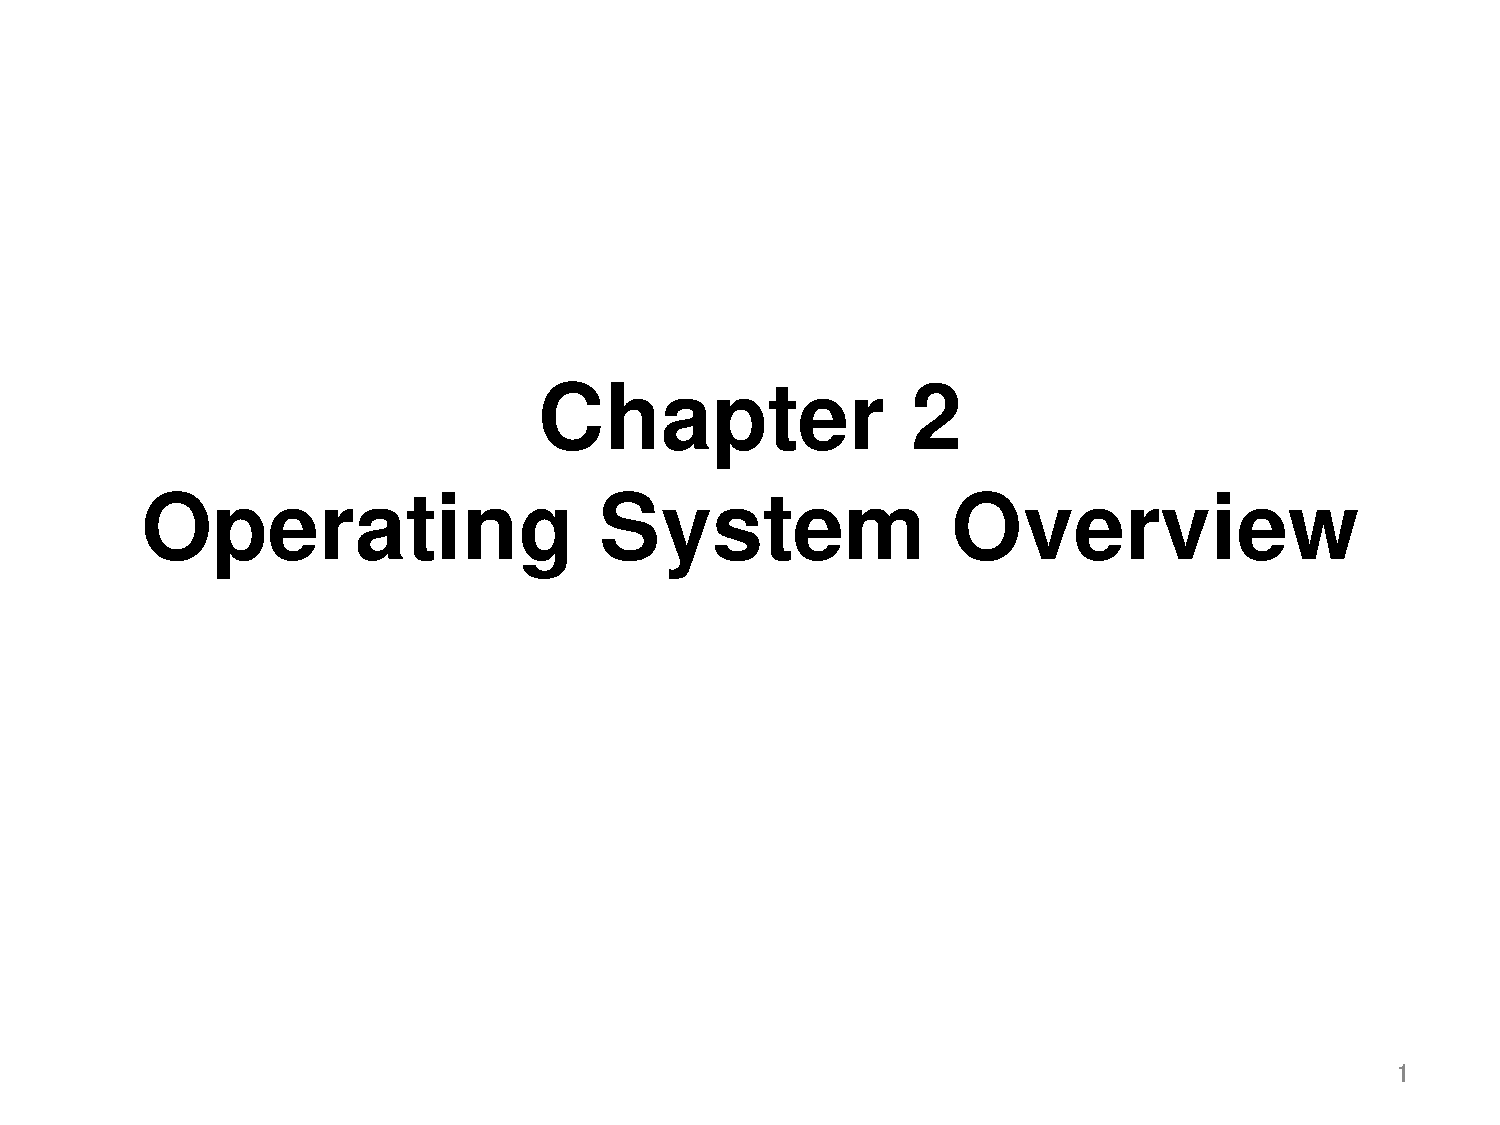
\includepdf[page=39]{03.pdf}
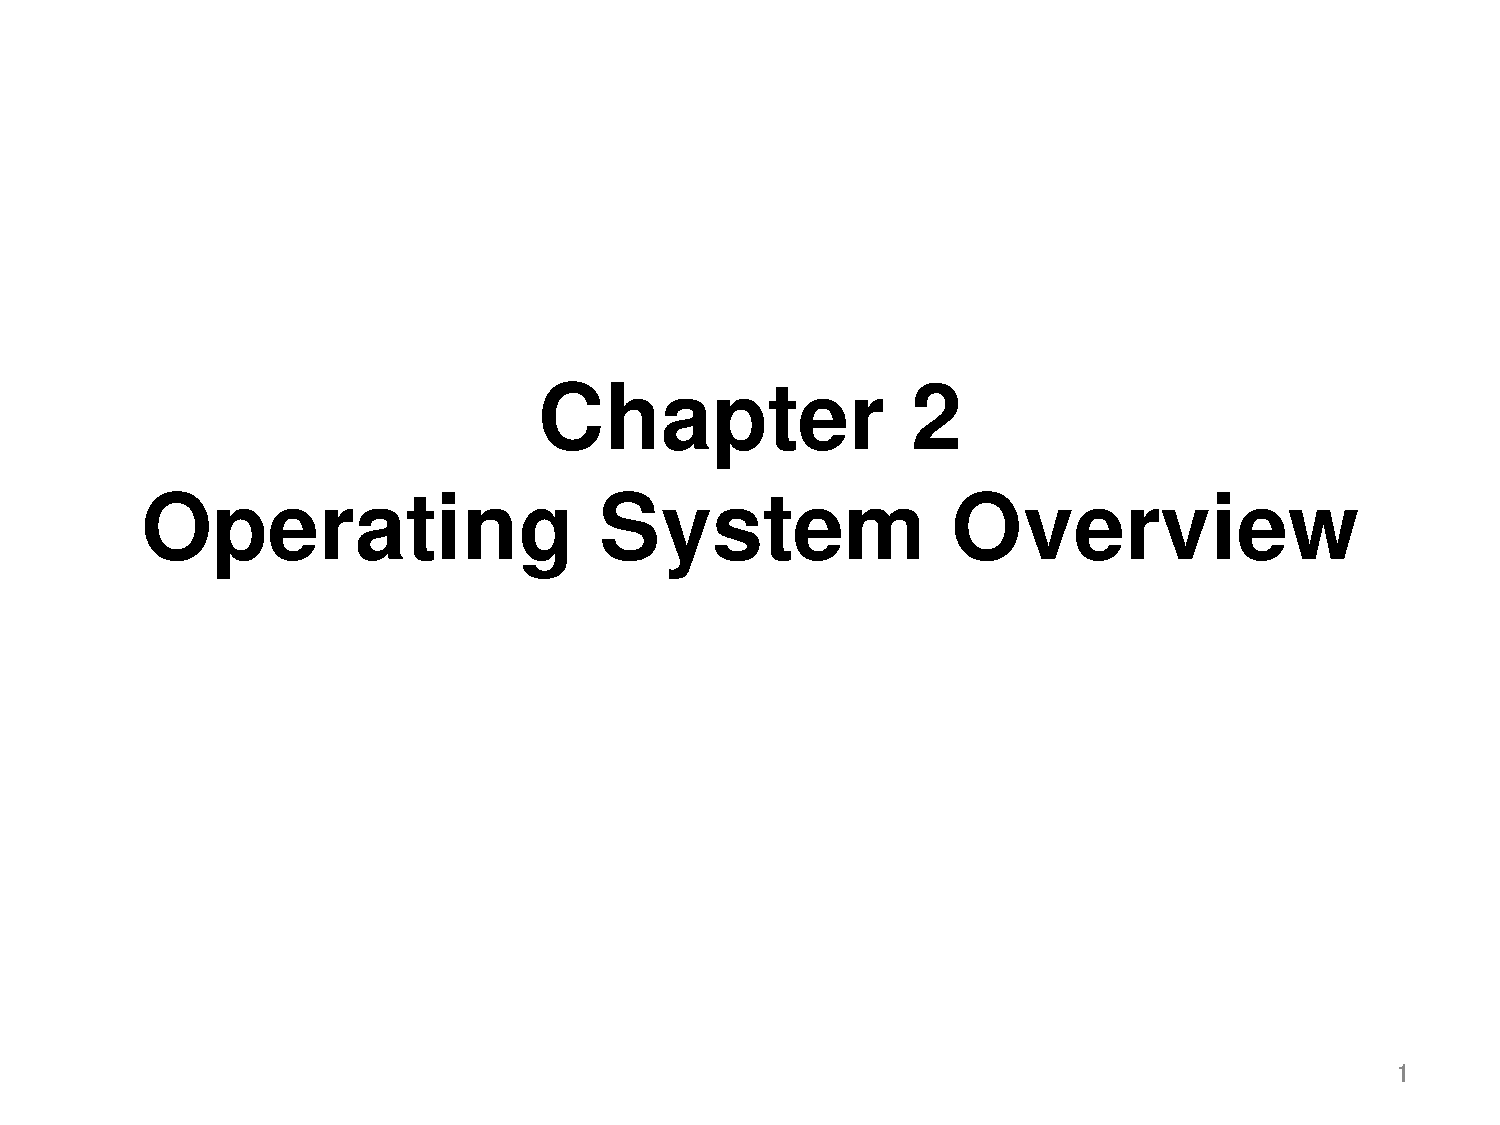
\includepdf[page=40]{03.pdf}
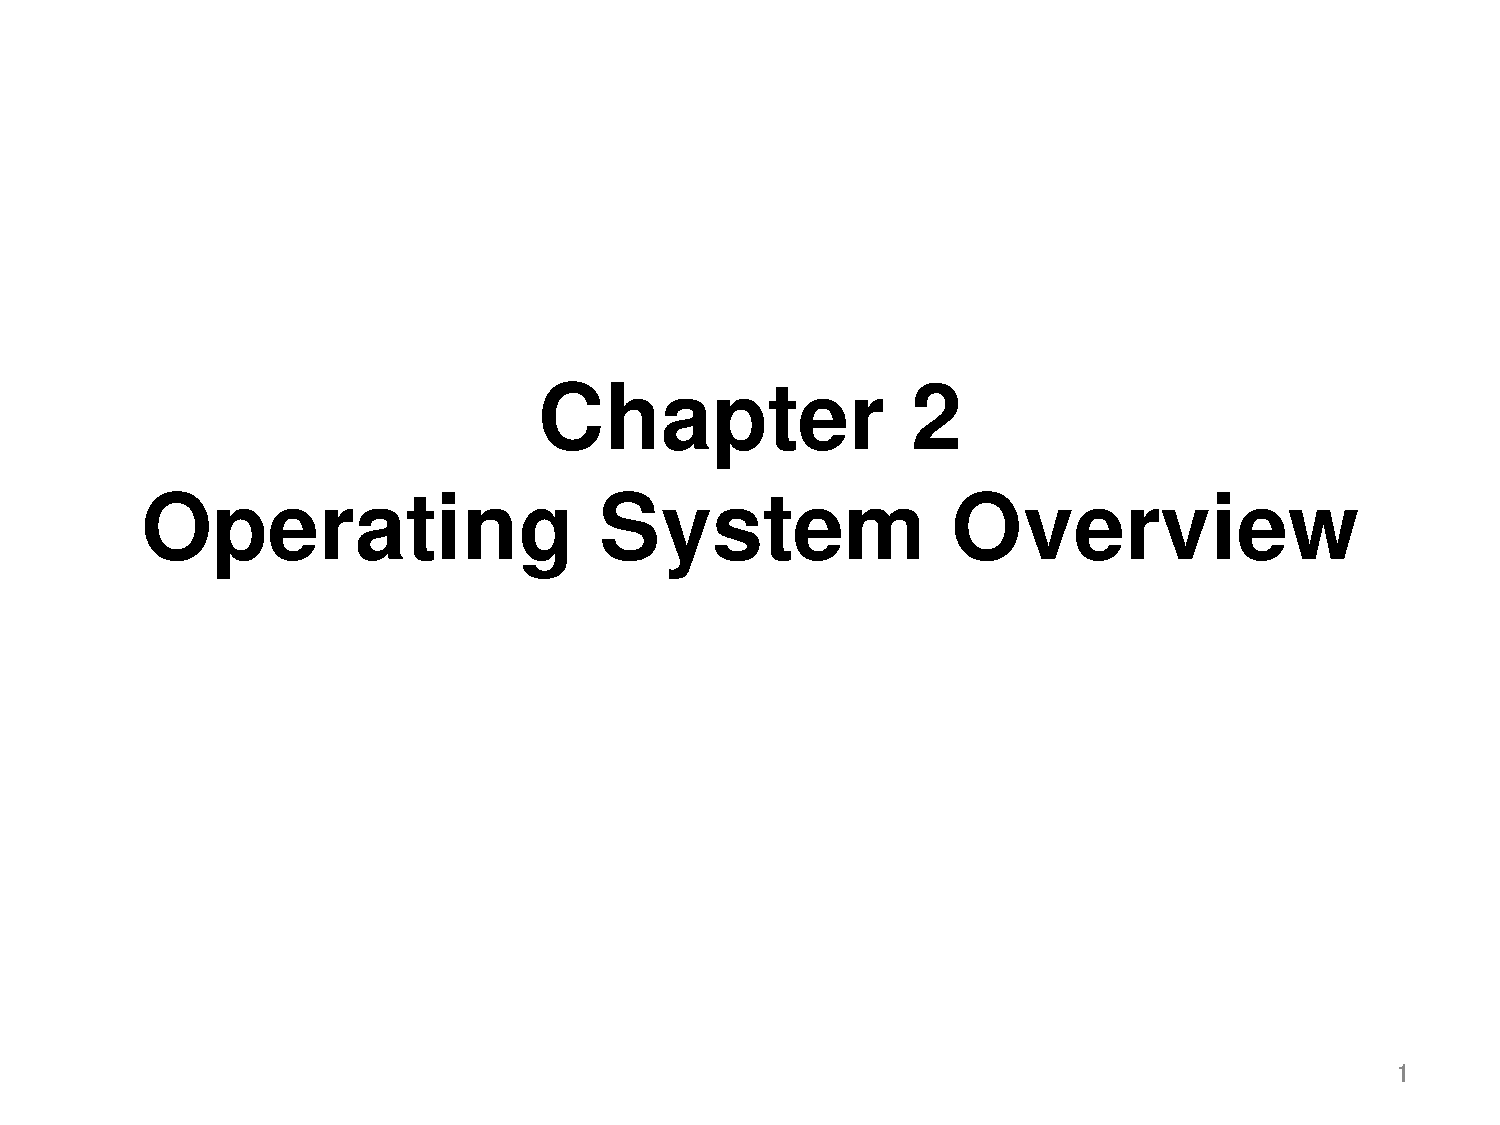
\includepdf[page=41]{03.pdf}
We need to worry about confidentiality, we dont want users to be able to fuck with each other's data. Along with this we need the ability to correctly test if a user is who they say they are.
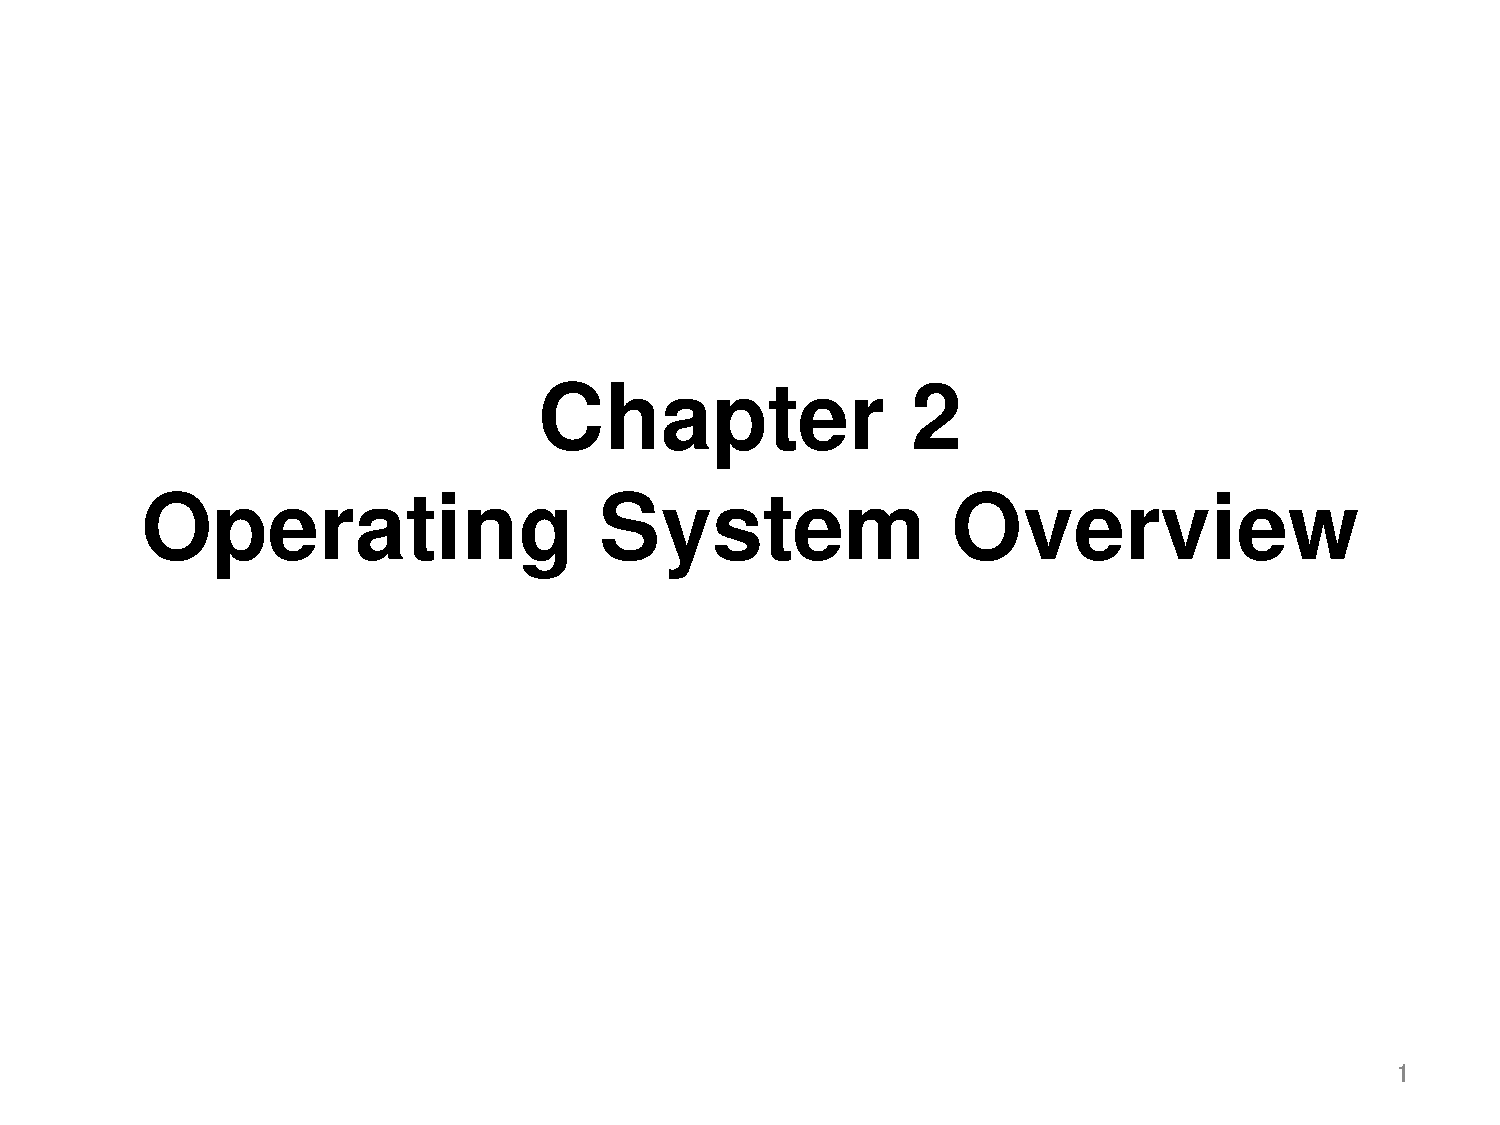
\includepdf[page=42]{03.pdf}
Once we have multiple users or proceses we need to make sure that each can use the resoures fairly, keeping priorities in mind. The OS needs to respond to the individual needs of the process. We want to give more processor time to process heavy programs and a larger share of the IO to IO heavy programs. Is hard to tell the amount needed at the start of the program, so we adapt overtime how resources are allocated.
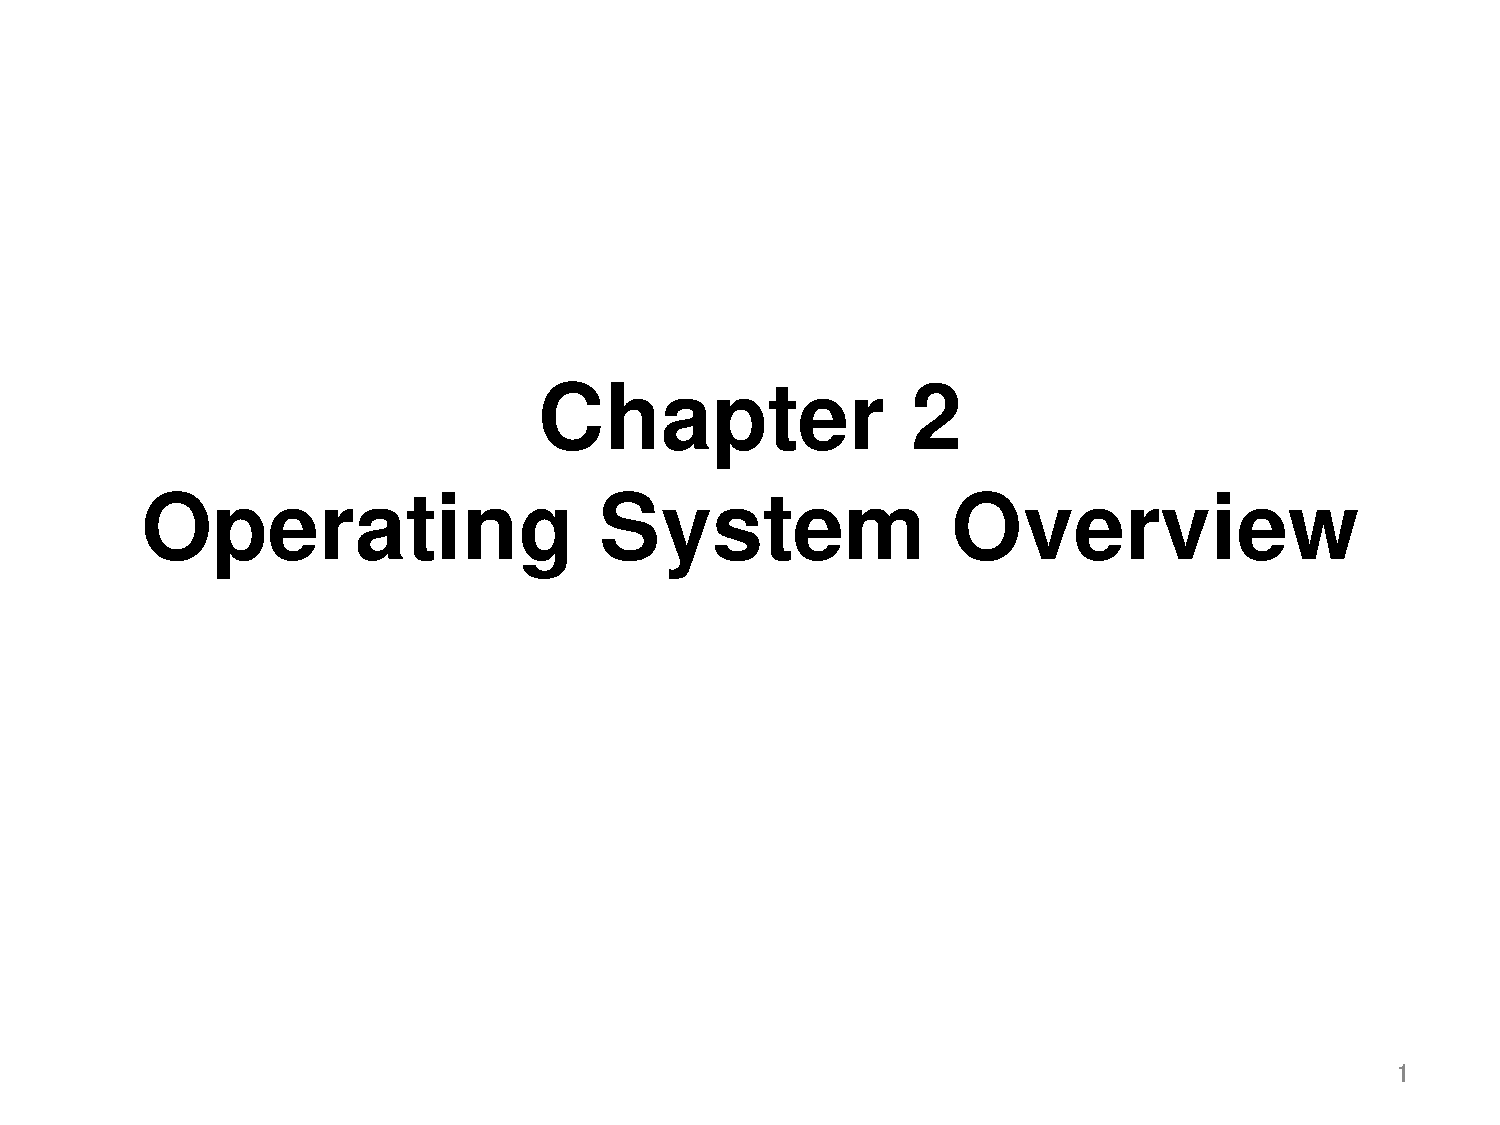
\includepdf[page=43]{03.pdf}
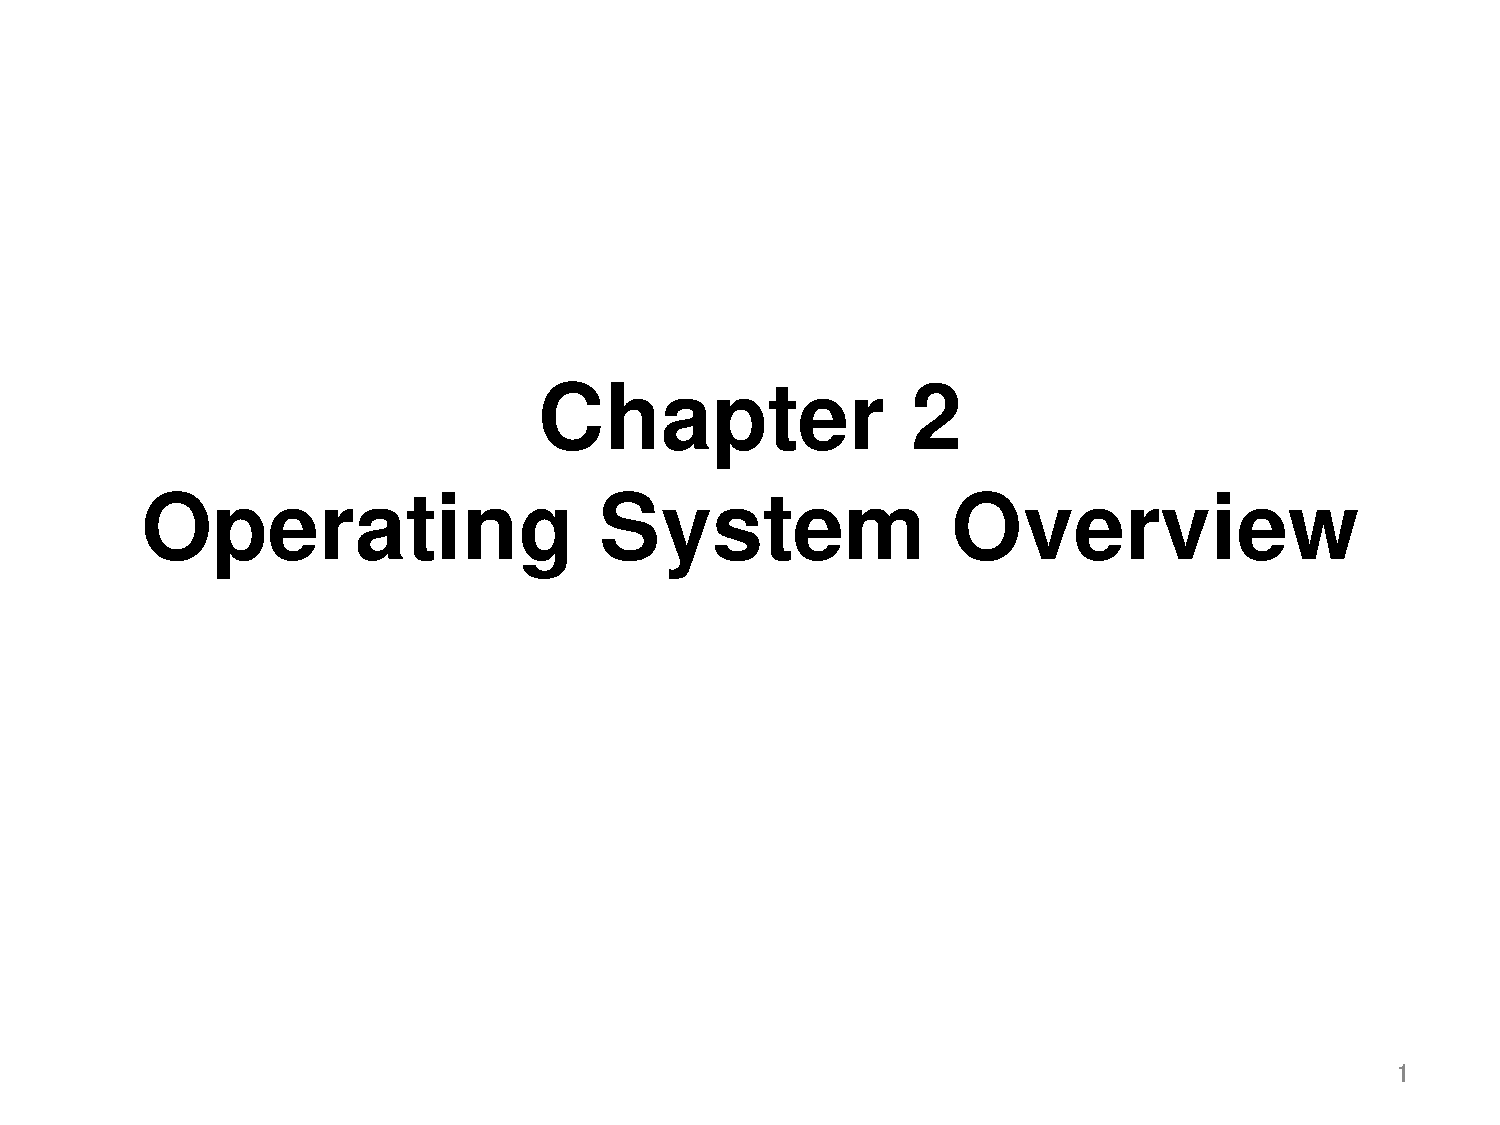
\includepdf[page=44]{03.pdf}
The long term queue contains the new processes and the short term queue holds ones that are ready to run. The IO queue holds processes that are blocked by the IO. The short term schedular helps to manage which process get what amount of resources.
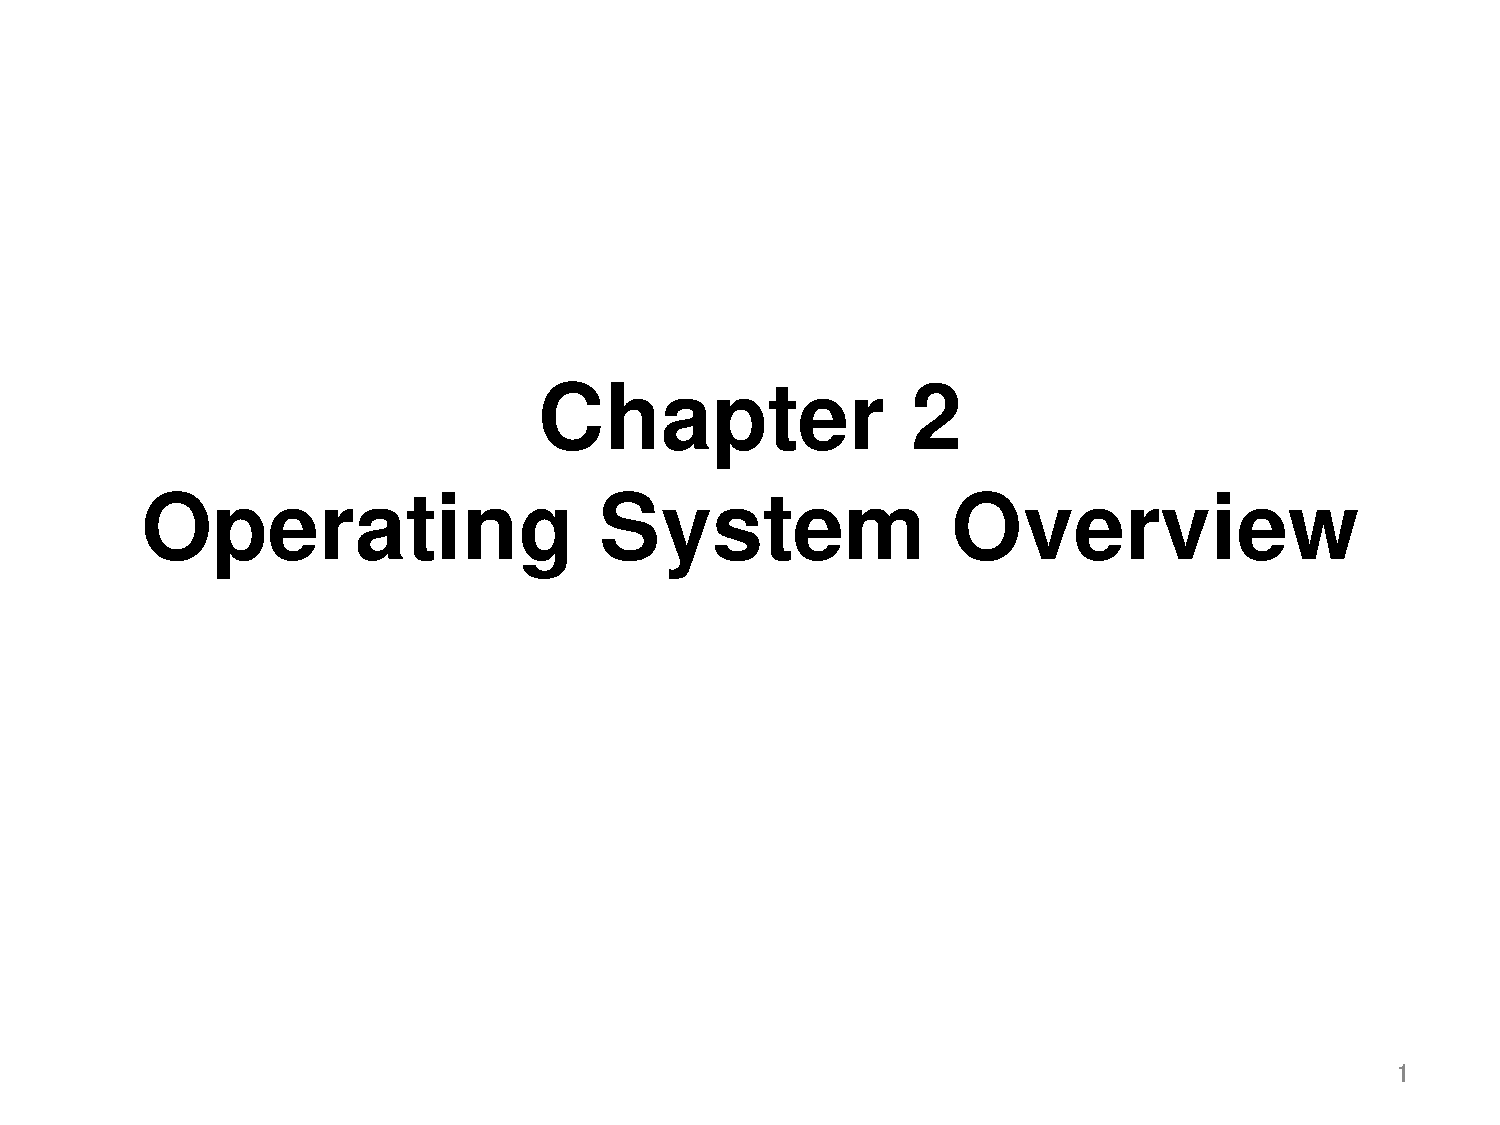
\includepdf[page=45]{03.pdf}
Os's have a lot of problems. Latent bugs and slow performance are big things. OS are huge peices of code making them hard to maintain which is why system structure is a big jump.
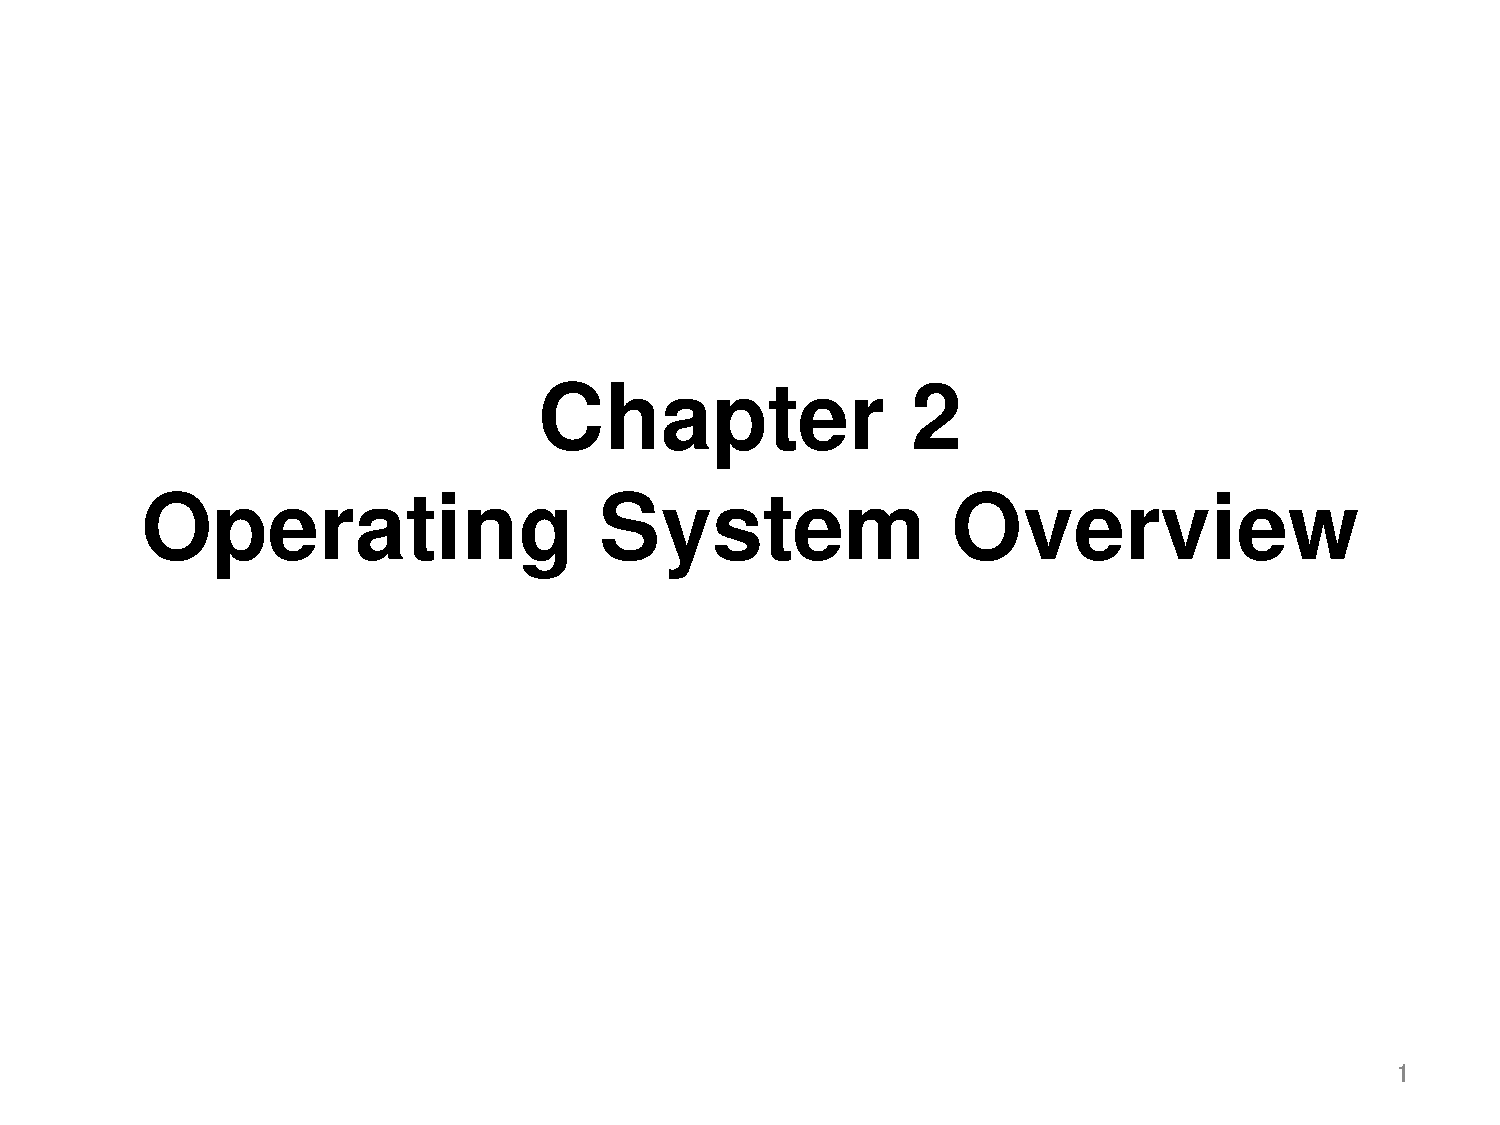
\includepdf[page=46]{03.pdf}
Each system are a series of levels where each level is a related subset of functions and relies on the next lowest level. This way we have a much simpler implementation
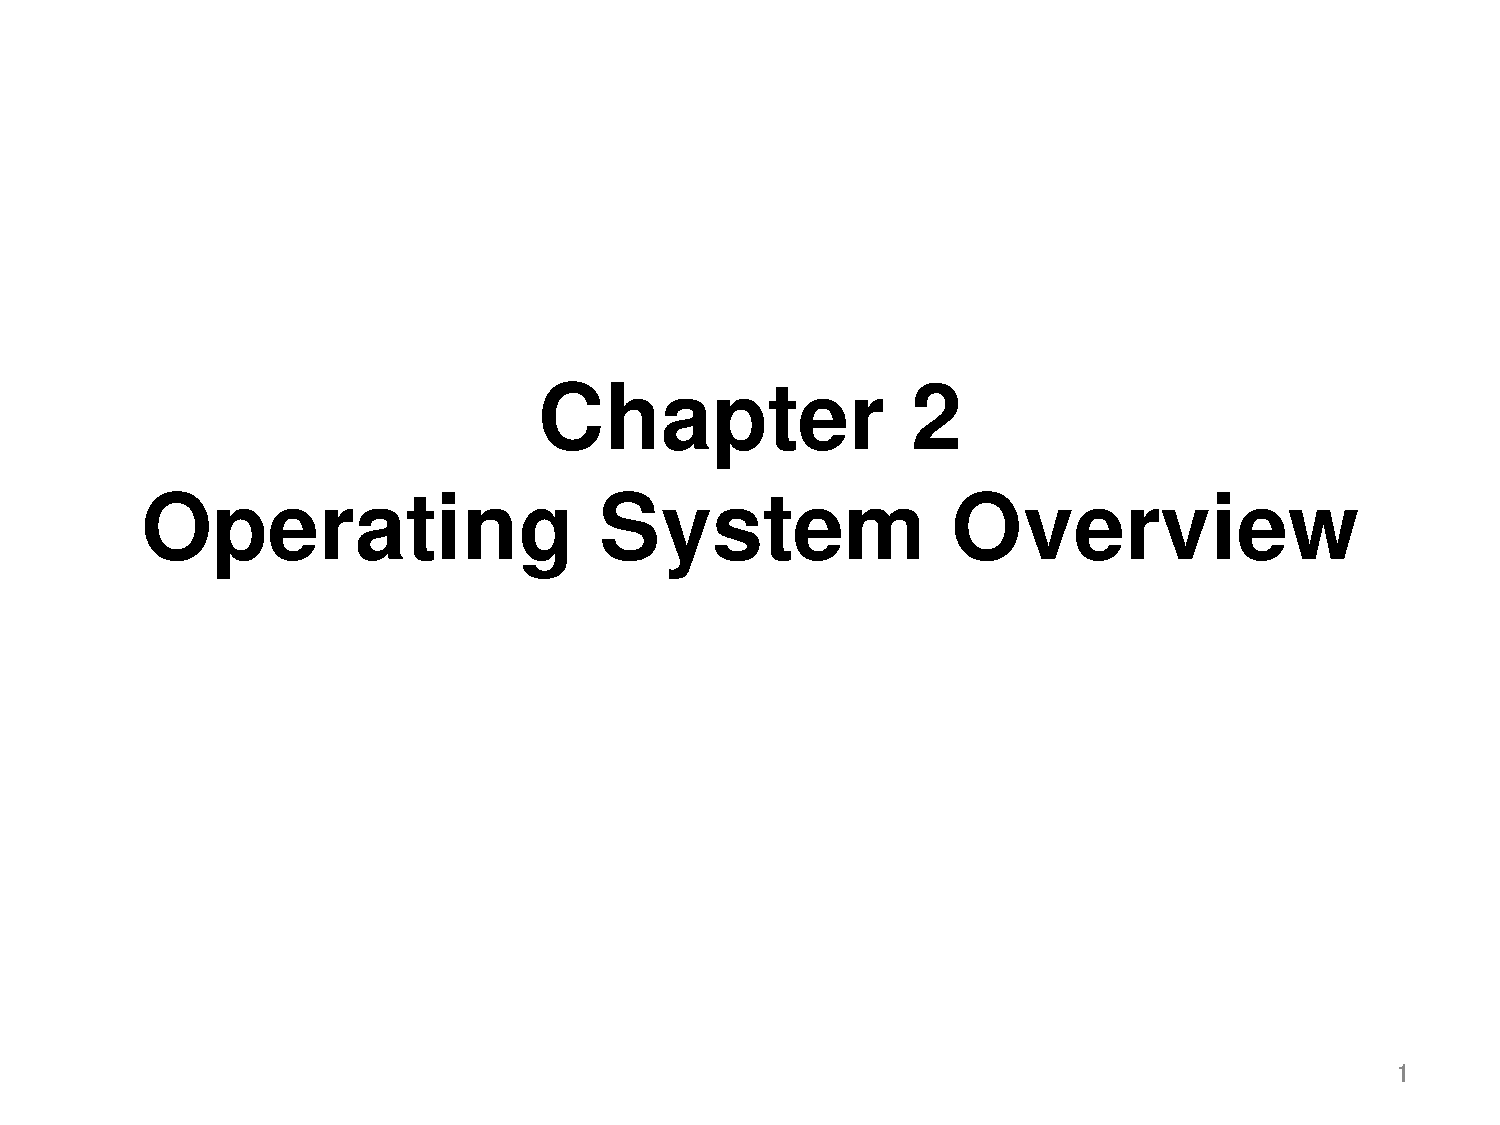
\includepdf[page=47]{03.pdf}
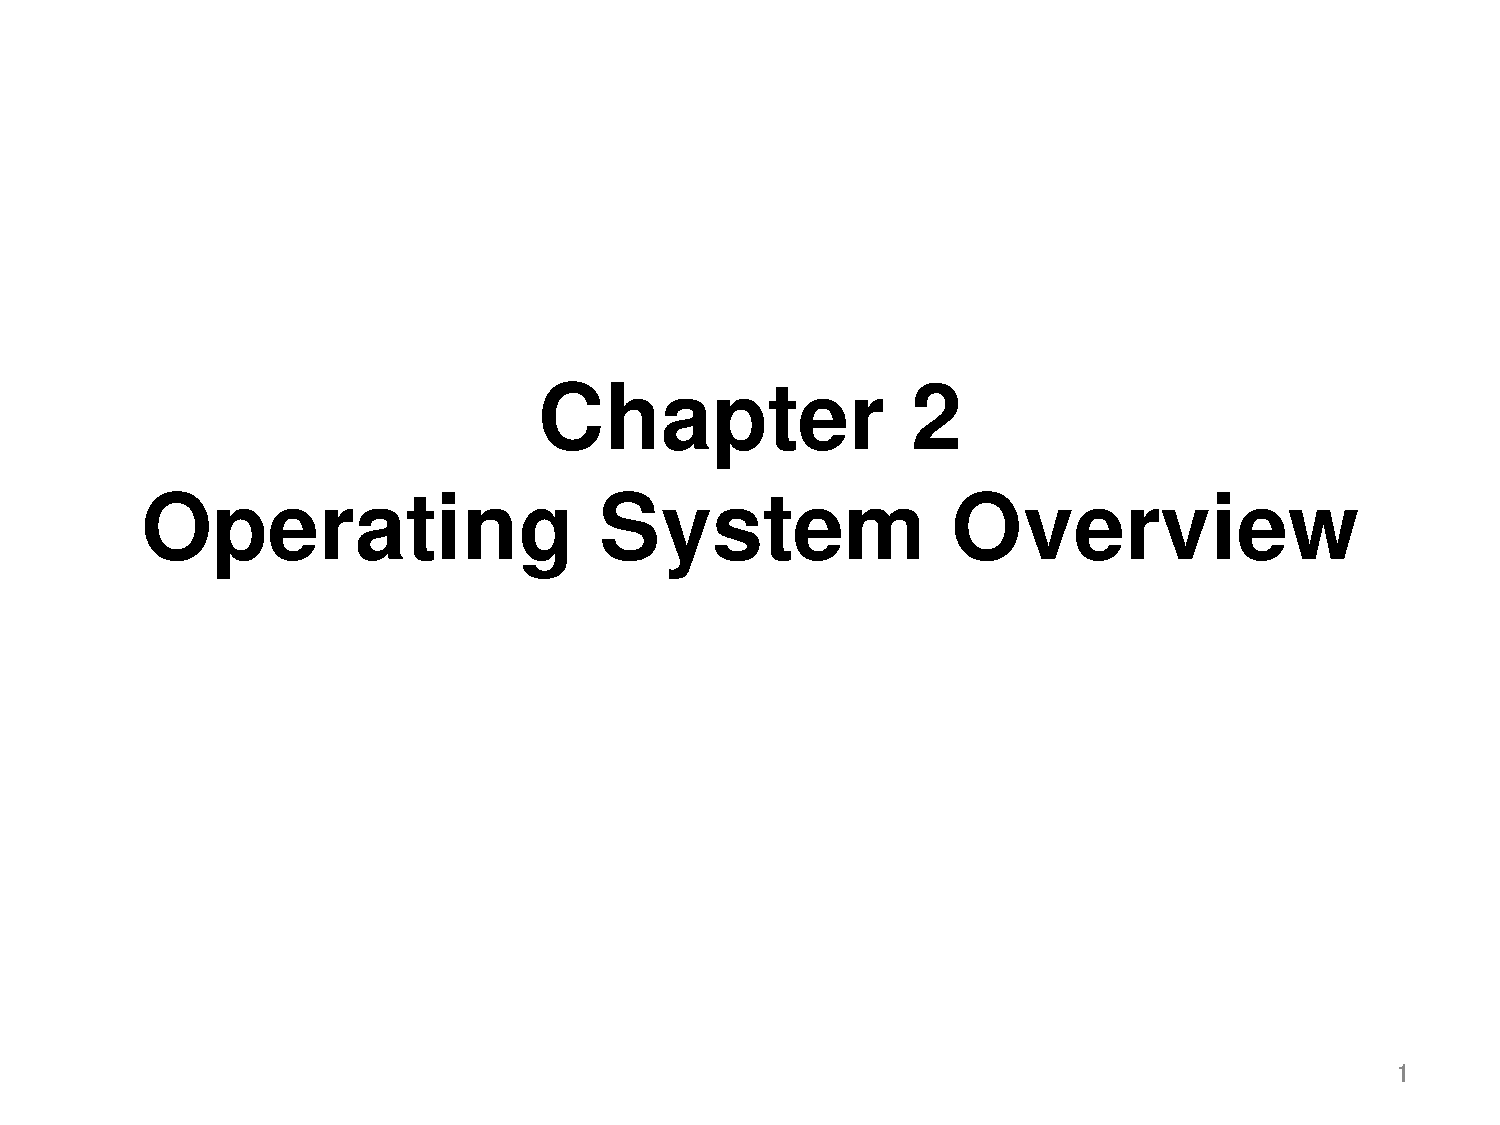
\includepdf[page=48]{03.pdf}
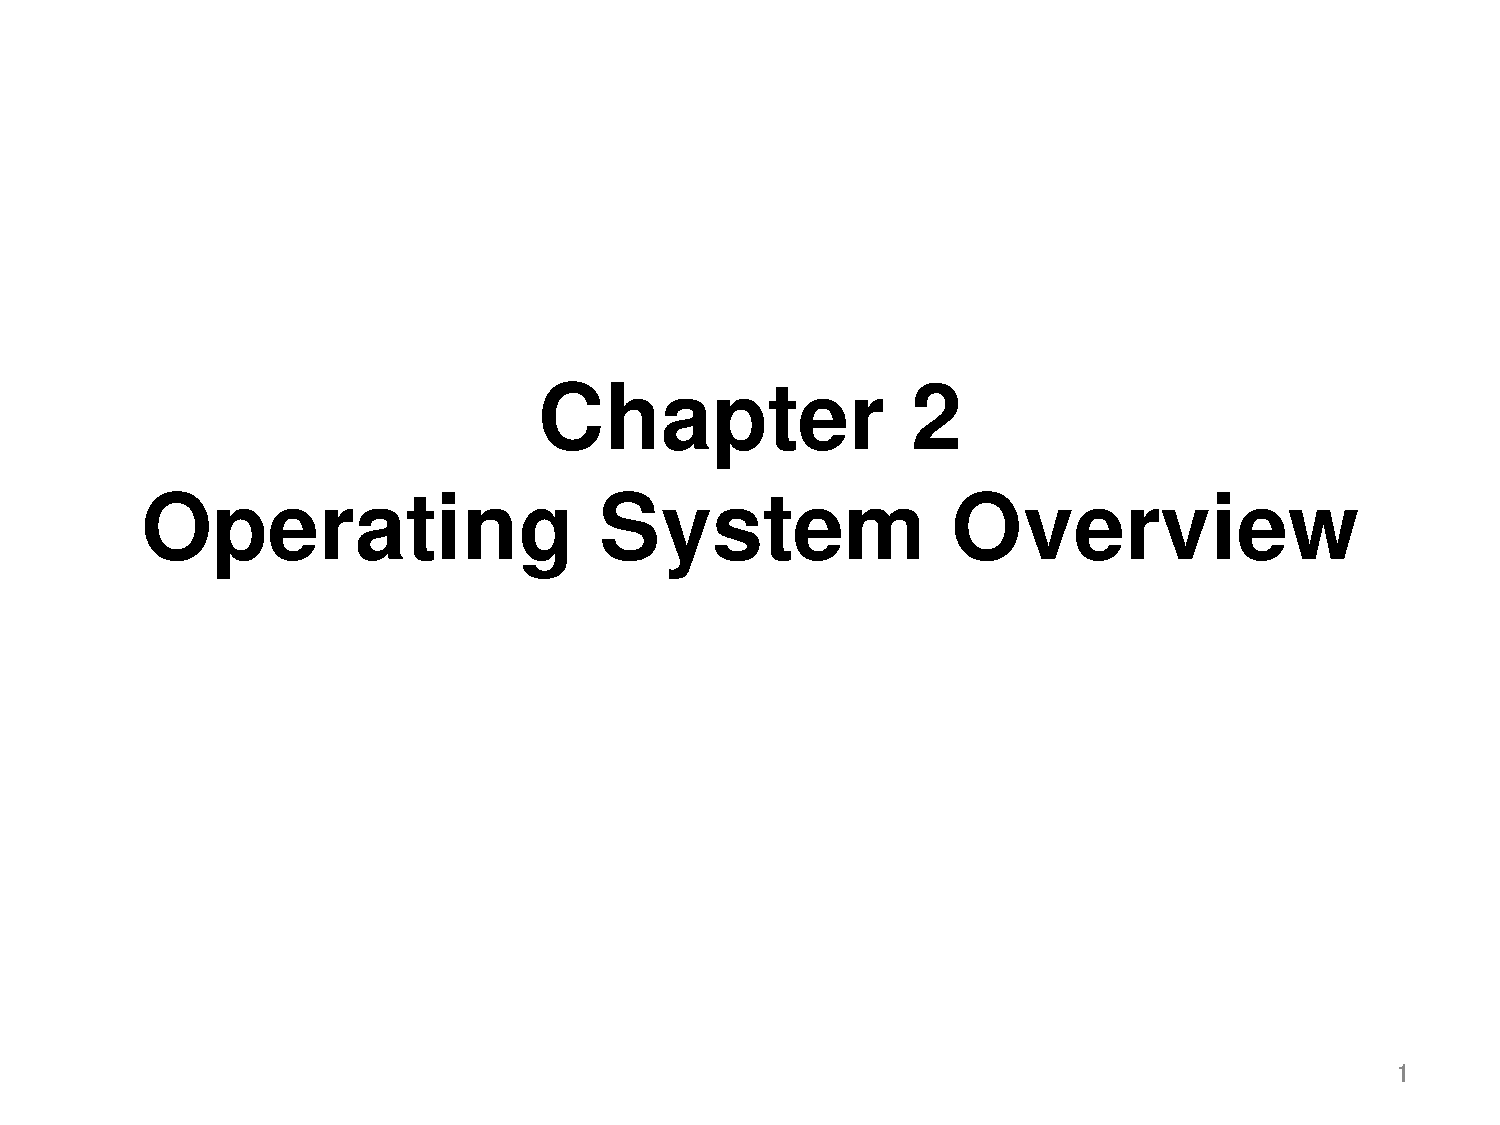
\includepdf[page=49]{03.pdf}
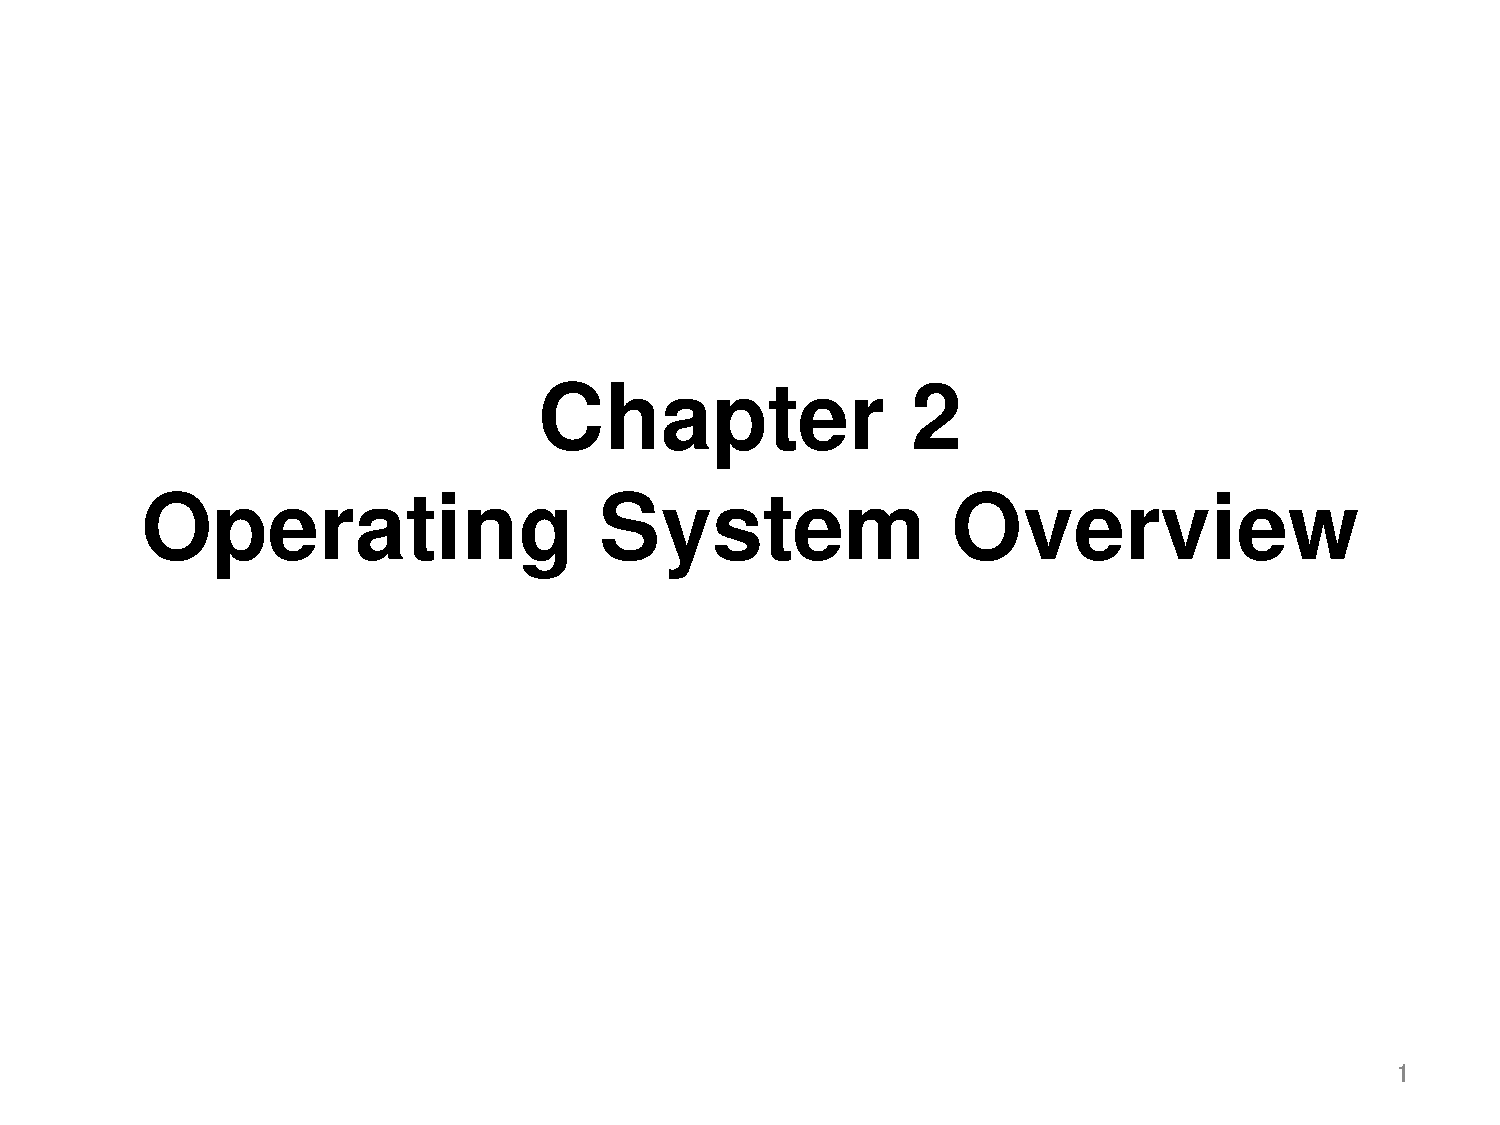
\includepdf[page=50]{03.pdf}
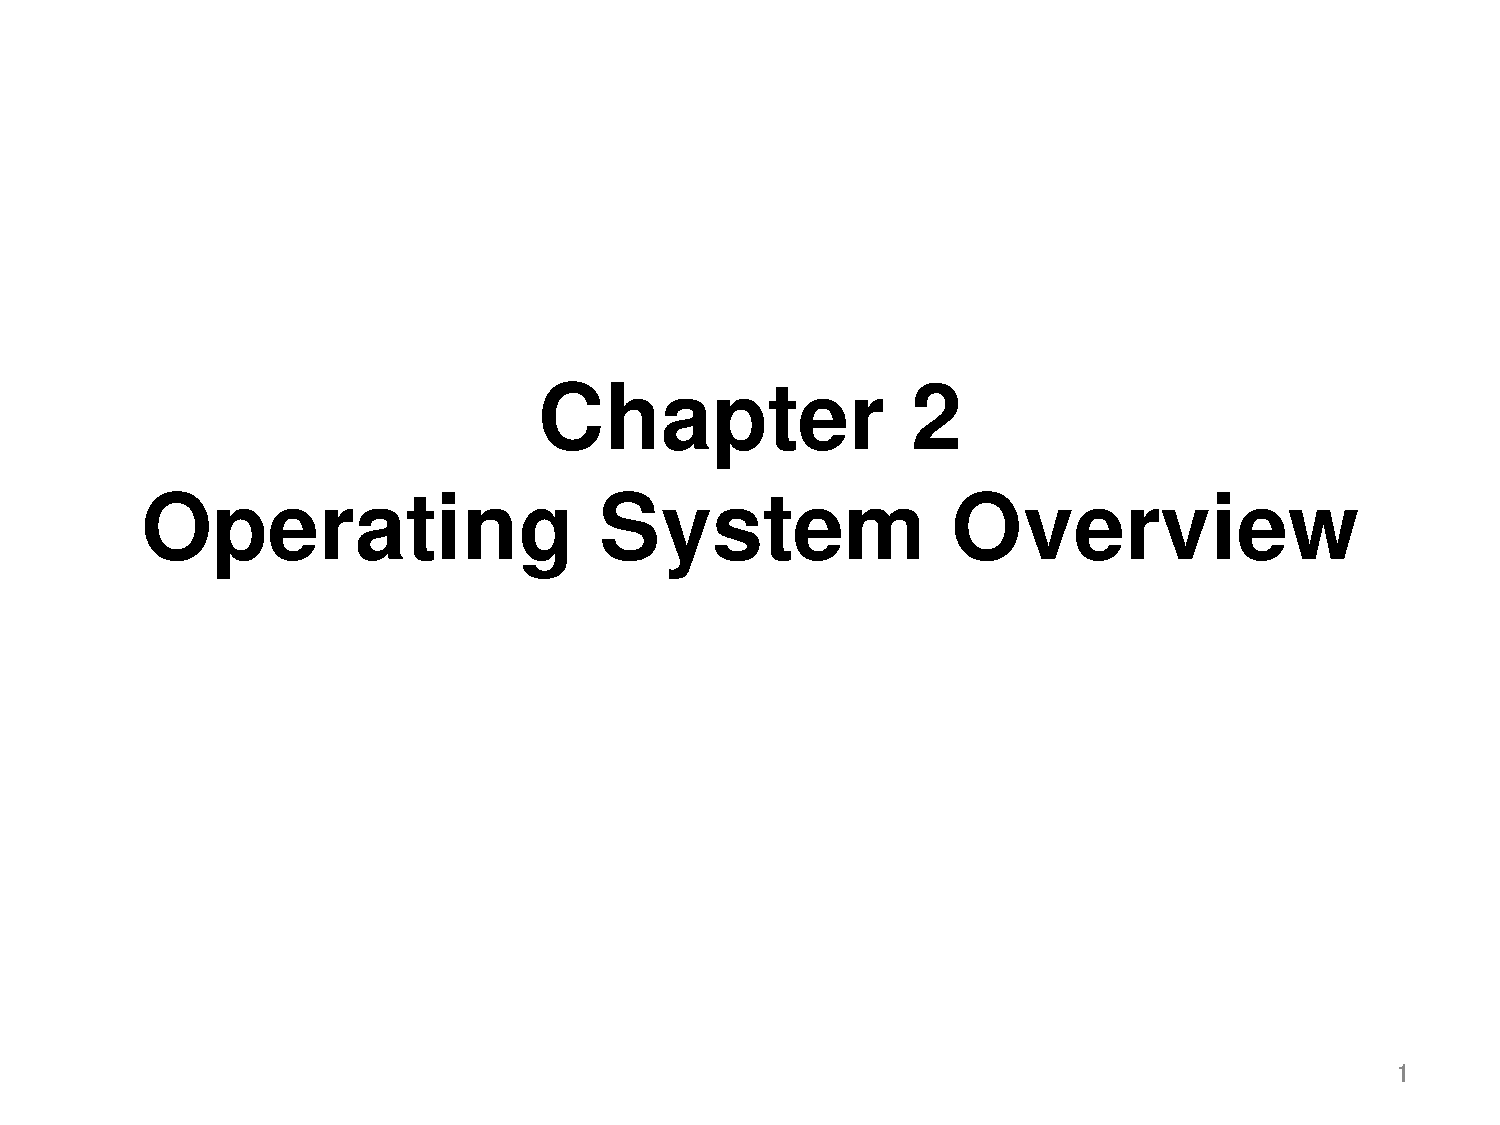
\includepdf[page=51]{03.pdf}
\includepdf[page=52]{03.pdf}
\includepdf[page=53]{03.pdf}
\includepdf[page=55]{03.pdf}
The kernel has very few operations and we expand off of these. Debugging microkernel os is very finicky and hard to work with, research is being done.
\includepdf[page=56]{03.pdf}
Multithreading is awesome. This lets us diving the process into concurrent threads which are interruptable. A process is just a collection of threads, but the pocess is the one in charge of memory management.
\includepdf[page=57]{03.pdf}
Mondern computer processors have multiple processors which share memory and threads which requires a whole bunch of code by the OS to use these most efficiently.
\includepdf[page=58]{03.pdf}
\includepdf[page=59]{03.pdf}
A distrubuted network uses multiple chips to let processes communicate and can be gamed to make it seem like there are more resources. Big-little means one large process with little ones next to it that we can move all of the heavy tasks to to make it seem like the little ones are much faster. Ex a quadcore processor. There are four big processor that are being used to run the apps and other things. There are a couple little micorcontrollers that are doing simple tasks. WE can use this to manage power by killing specific processors that are too intensive.

\textbf{Definition: } coupling (relatively) slower, low-power processor cores with (relatively) more powerful and power-hungry ones. The intention is to create a multi-core processor that can adjust better to dynamic computing needs and use less power than clock scaling alone.
\includepdf[page=60]{03.pdf}




\end{document}
